% Options for packages loaded elsewhere
\PassOptionsToPackage{unicode}{hyperref}
\PassOptionsToPackage{hyphens}{url}
\PassOptionsToPackage{dvipsnames,svgnames,x11names}{xcolor}
\documentclass[
  12pt,
]{book}
\usepackage{xcolor}
\usepackage[margin=3cm]{geometry}
\usepackage{amsmath,amssymb}
\setcounter{secnumdepth}{5}
\usepackage{iftex}
\ifPDFTeX
  \usepackage[T1]{fontenc}
  \usepackage[utf8]{inputenc}
  \usepackage{textcomp} % provide euro and other symbols
\else % if luatex or xetex
  \usepackage{unicode-math} % this also loads fontspec
  \defaultfontfeatures{Scale=MatchLowercase}
  \defaultfontfeatures[\rmfamily]{Ligatures=TeX,Scale=1}
\fi
\usepackage{lmodern}
\ifPDFTeX\else
  % xetex/luatex font selection
\fi
% Use upquote if available, for straight quotes in verbatim environments
\IfFileExists{upquote.sty}{\usepackage{upquote}}{}
\IfFileExists{microtype.sty}{% use microtype if available
  \usepackage[]{microtype}
  \UseMicrotypeSet[protrusion]{basicmath} % disable protrusion for tt fonts
}{}
\makeatletter
\@ifundefined{KOMAClassName}{% if non-KOMA class
  \IfFileExists{parskip.sty}{%
    \usepackage{parskip}
  }{% else
    \setlength{\parindent}{0pt}
    \setlength{\parskip}{6pt plus 2pt minus 1pt}}
}{% if KOMA class
  \KOMAoptions{parskip=half}}
\makeatother
\usepackage{color}
\usepackage{fancyvrb}
\newcommand{\VerbBar}{|}
\newcommand{\VERB}{\Verb[commandchars=\\\{\}]}
\DefineVerbatimEnvironment{Highlighting}{Verbatim}{commandchars=\\\{\}}
% Add ',fontsize=\small' for more characters per line
\usepackage{framed}
\definecolor{shadecolor}{RGB}{248,248,248}
\newenvironment{Shaded}{\begin{snugshade}}{\end{snugshade}}
\newcommand{\AlertTok}[1]{\textcolor[rgb]{0.94,0.16,0.16}{#1}}
\newcommand{\AnnotationTok}[1]{\textcolor[rgb]{0.56,0.35,0.01}{\textbf{\textit{#1}}}}
\newcommand{\AttributeTok}[1]{\textcolor[rgb]{0.13,0.29,0.53}{#1}}
\newcommand{\BaseNTok}[1]{\textcolor[rgb]{0.00,0.00,0.81}{#1}}
\newcommand{\BuiltInTok}[1]{#1}
\newcommand{\CharTok}[1]{\textcolor[rgb]{0.31,0.60,0.02}{#1}}
\newcommand{\CommentTok}[1]{\textcolor[rgb]{0.56,0.35,0.01}{\textit{#1}}}
\newcommand{\CommentVarTok}[1]{\textcolor[rgb]{0.56,0.35,0.01}{\textbf{\textit{#1}}}}
\newcommand{\ConstantTok}[1]{\textcolor[rgb]{0.56,0.35,0.01}{#1}}
\newcommand{\ControlFlowTok}[1]{\textcolor[rgb]{0.13,0.29,0.53}{\textbf{#1}}}
\newcommand{\DataTypeTok}[1]{\textcolor[rgb]{0.13,0.29,0.53}{#1}}
\newcommand{\DecValTok}[1]{\textcolor[rgb]{0.00,0.00,0.81}{#1}}
\newcommand{\DocumentationTok}[1]{\textcolor[rgb]{0.56,0.35,0.01}{\textbf{\textit{#1}}}}
\newcommand{\ErrorTok}[1]{\textcolor[rgb]{0.64,0.00,0.00}{\textbf{#1}}}
\newcommand{\ExtensionTok}[1]{#1}
\newcommand{\FloatTok}[1]{\textcolor[rgb]{0.00,0.00,0.81}{#1}}
\newcommand{\FunctionTok}[1]{\textcolor[rgb]{0.13,0.29,0.53}{\textbf{#1}}}
\newcommand{\ImportTok}[1]{#1}
\newcommand{\InformationTok}[1]{\textcolor[rgb]{0.56,0.35,0.01}{\textbf{\textit{#1}}}}
\newcommand{\KeywordTok}[1]{\textcolor[rgb]{0.13,0.29,0.53}{\textbf{#1}}}
\newcommand{\NormalTok}[1]{#1}
\newcommand{\OperatorTok}[1]{\textcolor[rgb]{0.81,0.36,0.00}{\textbf{#1}}}
\newcommand{\OtherTok}[1]{\textcolor[rgb]{0.56,0.35,0.01}{#1}}
\newcommand{\PreprocessorTok}[1]{\textcolor[rgb]{0.56,0.35,0.01}{\textit{#1}}}
\newcommand{\RegionMarkerTok}[1]{#1}
\newcommand{\SpecialCharTok}[1]{\textcolor[rgb]{0.81,0.36,0.00}{\textbf{#1}}}
\newcommand{\SpecialStringTok}[1]{\textcolor[rgb]{0.31,0.60,0.02}{#1}}
\newcommand{\StringTok}[1]{\textcolor[rgb]{0.31,0.60,0.02}{#1}}
\newcommand{\VariableTok}[1]{\textcolor[rgb]{0.00,0.00,0.00}{#1}}
\newcommand{\VerbatimStringTok}[1]{\textcolor[rgb]{0.31,0.60,0.02}{#1}}
\newcommand{\WarningTok}[1]{\textcolor[rgb]{0.56,0.35,0.01}{\textbf{\textit{#1}}}}
\usepackage{longtable,booktabs,array}
\usepackage{calc} % for calculating minipage widths
% Correct order of tables after \paragraph or \subparagraph
\usepackage{etoolbox}
\makeatletter
\patchcmd\longtable{\par}{\if@noskipsec\mbox{}\fi\par}{}{}
\makeatother
% Allow footnotes in longtable head/foot
\IfFileExists{footnotehyper.sty}{\usepackage{footnotehyper}}{\usepackage{footnote}}
\makesavenoteenv{longtable}
\usepackage{graphicx}
\makeatletter
\newsavebox\pandoc@box
\newcommand*\pandocbounded[1]{% scales image to fit in text height/width
  \sbox\pandoc@box{#1}%
  \Gscale@div\@tempa{\textheight}{\dimexpr\ht\pandoc@box+\dp\pandoc@box\relax}%
  \Gscale@div\@tempb{\linewidth}{\wd\pandoc@box}%
  \ifdim\@tempb\p@<\@tempa\p@\let\@tempa\@tempb\fi% select the smaller of both
  \ifdim\@tempa\p@<\p@\scalebox{\@tempa}{\usebox\pandoc@box}%
  \else\usebox{\pandoc@box}%
  \fi%
}
% Set default figure placement to htbp
\def\fps@figure{htbp}
\makeatother
\setlength{\emergencystretch}{3em} % prevent overfull lines
\providecommand{\tightlist}{%
  \setlength{\itemsep}{0pt}\setlength{\parskip}{0pt}}
\usepackage[]{natbib}
\bibliographystyle{apalike}
\usepackage{booktabs}
\usepackage{booktabs}
\usepackage{caption}
\usepackage{longtable}
\usepackage{colortbl}
\usepackage{array}
\usepackage{anyfontsize}
\usepackage{multirow}
\usepackage{bookmark}
\IfFileExists{xurl.sty}{\usepackage{xurl}}{} % add URL line breaks if available
\urlstyle{same}
\hypersetup{
  pdftitle={Fundamentos estadísticos para el análisis de las encuestas postcensales},
  pdfauthor={Andrés Gutiérrez, Giovany Babativa-Márquez},
  colorlinks=true,
  linkcolor={blue},
  filecolor={Maroon},
  citecolor={Blue},
  urlcolor={Blue},
  pdfcreator={LaTeX via pandoc}}

\title{Fundamentos estadísticos para el análisis de las encuestas postcensales}
\author{Andrés Gutiérrez\footnote{Comisión Económica para América Latina y el Caribe (CEPAL) - \href{mailto:andres.gutierrez@cepal.org}{\nolinkurl{andres.gutierrez@cepal.org}}}, Giovany Babativa-Márquez}
\date{2025-09-24}

\begin{document}
\maketitle

{
\hypersetup{linkcolor=}
\setcounter{tocdepth}{0}
\tableofcontents
}
\listoffigures
\listoftables
\chapter*{Abstract}\label{abstract}
\addcontentsline{toc}{chapter}{Abstract}

Este es el repositorio inicial para la Serie de Estudios Estadísticos sobre el análisis de las encuestas post-censales para la medición de la cobertura en los censos de población

\chapter{El sistema de estimación dual}\label{cap-dual}

Para poder hacer un análisis estadístico apropiado de las encuestas de cobertura como instrumentos que pretenden medir la omisión de un censo, es necesario remitirse a los rudimentos originales de su proceso inferencial, el cual está basado en el sistema de estimación dual. Este enfoque fue primeramente utilizado en modelos de captura y recaptura que se originaron en el siglo XVII, con desarrollos modernos a partir de \citet{petersen1896}, \citet{lincoln1930} y \citet{schnabel1938}. La aplicación a eventos vitales humanos fue iniciada por el trabajo de \citet{sekar1949}.

Este capítulo pretende establecer las condiciones iniciales bajo las cuales es apropiado utilizar este enfoque, así como los supuestos que se deben cumplir para que esta metodología produzca estimadores insesgados y precisos.

\section{Planteamiento del problema}\label{planteamiento-del-problema}

\citet{wolter1986coverage} considera una población humana \(U\), de tamaño \(N\), el cual es fijo pero desconocido y es precisamente el parámetro de interés sobre el cual se requiere una inferencia precisa. En una primera instancia, se supone que se realiza un censo de la población en un momento específico en el tiempo, y que el censo intenta enumerar a cada individuo. Sin embargo, por diversas razones, algunos individuos no son contados en el censo. La diferencia entre el conteo censal y \(N\) se denotará como el \emph{error de cobertura}.

Una de las principales complicaciones del error de cobertura es que su magnitud no puede determinarse únicamente a partir de los datos del censo. Para cuantificar este error, es imprescindible disponer de información adicional, la cual se obtiene generalmente mediante una encuesta por muestreo aplicada a la misma población objetivo. Esta encuesta (conocida como encuesta de postenumeración o encuesta de cobertura) se realiza habitualmente después del censo, utilizando el mismo período de referencia temporal. La encuesta permite estimar la magnitud del error de cobertura al comparar los resultados obtenidos con los datos del censo, proporcionando así una medida más precisa y ajustada de la población real.

Inicialmente, considérese que la encuesta representa una enumeración completa de toda la población, lo cual no es cierto en la práctica, pero este paso es necesario para esclarecer las propiedades estadísticas del sistema de estimación dual. Por supuesto, en los próximos capítulos de este documento se abordarán los acercamientos necesarios para ajustar la inferencia al caso real en el que la encuesta únicamente llega a una fracción de la población.

\section{Condiciones y supuestos}\label{condiciones-y-supuestos}

El modelo del error de cobertura descansa bajo un número de supuestos que son imprescindibles a la hora de utilizar una encuesta de postenumeración como instrumento fiable para la medición del error de cobertura en un censo. A continuación se realiza un listado exhaustivo de ellos.

\subsection{Estabilidad poblacional}\label{estabilidad-poblacional}

Se supone que la población \(U\) es cerrada y de tamaño fijo \(N\). En la práctica, esto implica que:

\begin{enumerate}
\def\labelenumi{\arabic{enumi}.}
\item
  El período de referencia del censo está bien definido; es decir que el censo se lleva a cabo en un intervalo de tiempo específico y claramente establecido. Este período es crucial para garantizar que todos los datos recolectados se refieran a la misma fecha o intervalo de tiempo, evitando así inconsistencias y errores en la estimación de la población.
\item
  No existen incorporaciones durante el período de referencia; es decir que se asume que no ocurren \textbf{nacimientos} ni \textbf{inmigraciones}. Esto significa que no se agregan nuevos individuos a la población censada.
\item
  No existen pérdidas; es decir que se asume que no ocurren \textbf{defunciones} ni \textbf{emigraciones} durante el período de referencia. Esto asegura que no se restan individuos de la población censada.
\end{enumerate}

\subsection{Estructura multinomial}\label{sec:multinomial}

El evento conjunto de que un individuo esté o no esté en el censo y esté o no en la encuesta se puede modelar correctamente usando una distribución multinomial con los siguientes parámetros:

\[
    \begin{array}{c|cc|c}
    & \text{En la encuesta} & \text{Fuera de la encuesta} & \text{Total} \\
    \hline
    \text{En el censo} & p_{11} & p_{12} & p_{1+} \\
    \text{Fuera del censo} & p_{21} & p_{22} & p_{2+} \\
    \hline
    \text{Total} & p_{+1} & p_{+2} & 1
    \end{array}
    \]

En donde:

\begin{itemize}
\tightlist
\item
  \(p_{11}\) denota la probabilidad de que un individuo sea encontrado en el censo y en la encuesta.
\item
  \(p_{12}\) denota la probabilidad de que un individuo sea encontrado en el censo, pero no en la encuesta.
\item
  \(p_{21}\) denota la probabilidad de que un individuo no sea encontrado en el censo, pero sí en la encuesta.
\item
  \(p_{22}\) denota la probabilidad de que un individuo no sea encontrado ni en el censo, ni en la encuesta.
\end{itemize}

Asimismo, en términos de las probabilidades marginales, se definen las siguientes cantidades:

\begin{itemize}
\tightlist
\item
  \(p_{1+}\) es la probabilidad de que un individuo sea correctamente encontrado en el censo.
\item
  \(p_{+1}\) es la probabilidad de que un individuo sea correctamente encontrado en la encuesta.
\end{itemize}

Esto quiere decir que el individuo tiene chance de ser clasificado en cualquiera de los cuatro estados definidos por las entradas de la tabla anterior; pero que al momento de la recolección de los datos, el individuo sólo puede pertenecer a uno y solo uno de estos estados.

\subsection{Independencia autónoma}\label{independencia-autuxf3noma}

El censo y la encuesta se generan como resultado de \(N\) ensayos mutuamente independientes. Cada ensayo representa a un individuo de la población real \(U\). A partir de la recolección de los datos, se obtiene la siguiente clasificación:

\[
    \begin{array}{c|cc|c}
    & \text{En la encuesta} & \text{Fuera de la encuesta} & \text{Total} \\
    \hline
    \text{En el censo} & N_{11} & N_{12} & N_{1+} \\
    \text{Fuera del censo} & N_{21} & N_{22} & N_{2+} \\
    \hline
    \text{Total} & N_{+1} & N_{+2} & N_{++} = N
    \end{array}
    \]

Note que \(N_{ab} = \sum_{k \in U} x_{kab}\) y \(x_{kab}\) es una variable indicadora que señala si el individuo \(k\) pertenece a la celda \((a, b)\) de la tabla \((a, b = 1,2,+)\). Bajo este esquema inicial, se tiene que:

\begin{enumerate}
\def\labelenumi{\arabic{enumi}.}
\tightlist
\item
  El conteo del censo \(N_{1+}\) se considera observable.
\item
  Los valores \(N_{11}\), \(N_{12}\) y \(N_{21}\) se consideran observables con base en los datos de la encuesta y el emparejamiento con el censo.
\item
  Los valores \(N_{22}\), y el tamaño de la población de interés \(N = N_{++}\), se consideran desconocidos y deben estimarse con base en el modelo.
\item
  Bajo este modelo, el conteo del censo \(N_{1+}\) define una variable aleatoria con media \(E(N_{1+}) = Np_{1+}\) y varianza \(V(N_{1+}) = Np_{1+}(1 - p_{1+})\).
\end{enumerate}

\subsection{Independencia causal}\label{independencia-causal}

Se supone que el evento de ser incluido en el censo es independiente del evento de ser incluido en la encuesta. Como resultado de este supuesto, la razón de productos cruzados de probabilidades, conocida comúnmente como la Razón de Odds, satisface la siguiente relación:

\[
\frac{p_{11} \cdot p_{22}}{p_{12} \cdot p_{21}} = 1
\]

El resultado anterior se tiene, puesto que la probabilidad conjunta de un individuo en una celda específica de la tabla de contingencia se factoriza como:

\[
p_{11} = P(\text{individuo está en el censo y en la encuesta}) = p_{1+} \cdot p_{+1}
\]

Similarmente, se tiene que

\[
p_{12} = p_{1+} \cdot (1 - p_{+1})
\]
\[
p_{21} = (1 - p_{i1+})\cdot p_{i+1}  p
\]

\[
p_{22} = (1 - p_{i1+}) \cdot (1 - p_{i+1})
\]
Sustituyendo adecuadamente en la razón de productos cruzados, entonces se tiene que

\[
\frac{p_{11} p_{22}}{p_{12} p_{21}} =
\frac{p_{1+} p_{+1} (1 - p_{1+}) (1 - p_{+1})}
{p_{1+} (1 - p_{+1}) (1 - p_{1+}) p_{+1}} = 1
\]

La dependencia causal, como señala el \citet{USCensusBureau_2022}, es un fenómeno que ocurre cuando la inclusión o exclusión de un individuo en el censo influye en su probabilidad de ser incluido en la encuesta. Este tipo de dependencia puede generar sesgos en los datos y afectar la calidad de las estimaciones estadísticas, lo que a su vez puede comprometer la validez de las conclusiones derivadas de estos estudios. Por ello, es fundamental implementar estrategias que mitiguen este riesgo y aseguren la independencia operativa entre ambos sistemas.

Una de las medidas clave para lograr esta independencia operativa es garantizar que el personal involucrado en la recolección de datos de la encuesta no participe en las mismas áreas geográficas o comunidades donde trabajaron durante el censo. Esto reduce la posibilidad de que los encuestadores influyan en las respuestas de los individuos basándose en interacciones previas o en información recopilada durante el censo. Además, al evitar la superposición de personal, se minimiza el riesgo de que los encuestados asocien ambas actividades, lo que podría alterar su disposición a participar o la veracidad de sus respuestas.

Otra estrategia importante es asegurar que las entrevistas de la encuesta se realicen después de que las operaciones del censo hayan concluido en un área específica. Esto permite que los procesos de recolección de datos no se solapen temporalmente, lo que reduce la posibilidad de que los resultados de una actividad afecten directa o indirectamente a la otra. Por ejemplo, si un individuo ha sido contactado recientemente para el censo, podría sentirse menos motivado a participar en la encuesta, o viceversa. Separar prudencialmente ambas operaciones ayuda a mantener la independencia de las respuestas.

Además, es crucial restringir el acceso del personal del censo a la información sobre la muestra de la encuesta. De manera similar, el personal de la encuesta no debería tener acceso a los resultados del censo durante la fase de recolección de datos, ya que esta información podría sesgar su enfoque o interpretación de las respuestas.

\subsection{Emparejamiento}\label{emparejamiento}

Se asume que es posible realizar un emparejamiento preciso entre los resultados de la encuesta y los del censo. Esto significa que se puede identificar de manera exacta y sin errores:

\begin{enumerate}
\def\labelenumi{\arabic{enumi}.}
\tightlist
\item
  Cuáles individuos registrados en la encuesta también aparecen en los registros del censo.
\item
  Cuáles individuos de la encuesta no están presentes en los datos del censo.
\end{enumerate}

Este emparejamiento correcto es crucial para evaluar la cobertura del censo y para ajustar las estimaciones de la población total, asegurando que los datos sean lo más precisos y completos posible.

Por otro lado, se asume que inevitablemente habrá algún grado de no respuesta en el censo y en la encuesta. Esto significa que algunos individuos no serán contactados o no proporcionarán la información solicitada. Para abordar este problema, es fundamental recopilar suficiente información auxiliar sobre los no respondientes. Esta información puede incluir datos como nombres, direcciones, fechas de nacimiento y otros identificadores únicos que permitan una correcta identificación de los individuos.

En la práctica, se implementan procedimientos específicos para asegurar que la información recopilada sea lo suficientemente detallada y precisa para permitir un emparejamiento exacto entre los datos del censo y los de la encuesta. Este emparejamiento es crucial para evaluar la cobertura del censo y ajustar las estimaciones de la población total.

\subsection{Eventos espurios}\label{eventos-espurios}

Se asume que tanto el censo como la encuesta están libres de incidencias espurias o falsas, o que estas han sido eliminadas antes de realizar las estimaciones. Esto implica que se han tomado medidas para evitar cualquier tipo de error en el registro de los resultados tanto del censo como de la encuesta. En la práctica, esto significa que se han implementado procedimientos rigurosos para identificar y corregir cualquier anomalía en los datos. Algunos de los eventos espurios más importantes que pueden ocurrir incluyen:

\begin{enumerate}
\def\labelenumi{\arabic{enumi}.}
\tightlist
\item
  Duplicaciones en la lista del censo. Esto ocurre cuando un individuo es contado más de una vez en el censo, lo que puede inflar artificialmente el tamaño de la población.
\item
  Registros de casos inexistentes. Estos son registros de individuos que no existen en realidad, pero que han sido incluidos erróneamente en el censo o en la encuesta. Esto puede suceder debido a errores de entrada de datos o malentendidos durante la recolección de información.
\item
  Casos no pertinentes. Estos son individuos que no deberían haber sido incluidos en el censo debido a que no cumplen con los criterios del período de referencia. Un ejemplo común es el registro de un individuo que nació después del período de referencia del censo, lo que resulta en una inclusión incorrecta en los datos.
\end{enumerate}

Para asegurar la precisión de las estimaciones, es crucial que estos eventos espurios sean identificados y eliminados antes de proceder con el análisis de los datos.

\subsection{Postestratificación}\label{postestratificaciuxf3n}

Es frecuente y beneficioso aplicar algún tipo de postestratificación en la estimación del tamaño real de la población. La postestratificación es una técnica estadística que permite ajustar las estimaciones de la población dividiéndola en subgrupos homogéneos, basados en variables categóricas. Esta técnica mejora la precisión y la validez de las estimaciones al considerar las diferencias dentro de la población.

Por ejemplo, una forma común de postestratificación es por edad. En este caso, la población se divide en diferentes grupos de edad, como niños, adolescentes, adultos jóvenes, adultos de mediana edad y personas mayores. Para cada uno de estos grupos de edad, se realizan estimaciones específicas de la población. Estas estimaciones se basan en los datos recolectados tanto en el censo como en la encuesta. Una vez obtenidas las estimaciones específicas por edad, se agregan para calcular una estimación total de la población, denotada como \(N\).

La postestratificación no se limita solo a la edad; también se puede aplicar a otras variables demográficas y socioeconómicas, como sexo, etnia, nivel educativo, región geográfica, entre otras. Es fundamental que cualquier variable utilizada para la postestratificación esté correctamente registrada para todos los individuos tanto en el censo como en la encuesta.

\section{Inferencia}\label{inferencia}

Nuestro objetivo es estimar el tamaño total de una población, denotado como \(N_{++}\), utilizando dos fuentes de información complementarias. La primera fuente es el censo, el cual logra capturar correctamente a \(N_{+1}\) individuos de la población. La segunda fuente es la encuesta, que captura de manera precisa a \(N_{1+}\) individuos.

Uno de los supuestos del sistema de estimación dual es que el evento de que una persona sea encontrada se puede modelar como un proceso estocástico de tipo Bernoulli. Esto quiere decir que \(N_{11}\), \(N_{1+}\) y \(N_{+1}\) se asumen como variables aleatorias binomiales al ser sumas de eventos Bernoulli.

\subsection{Los estimadores del sistema dual}\label{los-estimadores-del-sistema-dual}

Bajo este modelo, las variables aleatorias siguen distribuciones binomiales condicionales:

\[
N_{1+} \sim \text{Bin}(N_{++}, p_{1+}), \quad N_{+1} \sim \text{Bin}(N_{++}, p_{+1}), \quad N_{11} \sim \text{Bin}(N_{++}, p_{11})
\]

Una vez que los datos hayan sido recolectados y clasificados bajo este esquema, es bien sabido en la literatura estadística, que los estimadores para las probabilidades de interés toman la siguiente forma:

\[
\tilde{p}_{11} = \frac{N_{11}}{N_{++}},  \quad 
\tilde{p}_{1+} = \frac{N_{1+}}{N_{++}},  \quad 
\tilde{p}_{+1} = \frac{N_{+1}}{N_{++}}
\]

Al asumir independencia entre la captura en el censo y la captura en la encuesta, entonces \(\tilde{p}_{11} = \tilde{p}_{1+} \cdot \tilde{p}_{+1}\), y por ende:

\[
\frac{N_{11}}{N_{++}} = \frac{N_{1+}}{N_{++}} \cdot \frac{N_{+1}}{N_{++}}
\]

Luego, al despejar convenientemente, se encuentra que el estimador del sistema dual para el total poblacional \(N_{++}\) está dado por

\[
\tilde{N}_{++} = \frac{N_{1+} \cdot N_{+1}}{N_{11}} 
\]

A partir de este resultado, podemos reemplazar en las expresiones \(\tilde{p}_{11}\), \(\tilde{p}_{1+}\) y \(\tilde{p}_{+1}\) para obtener estimadores de máxima verosimilitud para las probabilidades de interés son los siguientes:

\[
\tilde{p}_{11} = \frac{N_{11}}{\tilde{N}_{++}} = \frac{N_{11}^2}{N_{1+} \cdot N_{+1}}
\]

\[
\tilde{p}_{1+} = \frac{N_{1+}}{\tilde{N}_{++}} = \frac{N_{11}}{N_{+1}}
\]

\[
\tilde{p}_{+1} = \frac{N_{+1}}{\tilde{N}_{++}} = \frac{N_{11}}{N_{1+}}
\]

\citet[sección 2.4]{wolter1986coverage} plantea un esquema conjunto que induce estos mismos estimadores a partir de la función de verosimilitud asociada al modelo, la cual está dada por la siguiente expresión:

\[
L(N, p_{i+}, p_{+i}) = \binom{N}{x_{11}, x_{12}, x_{21}} p_{1+}^{x_{1+}} (1 - p_{1+})^{N - x_{1+}} p_{+1}^{x_{+1}} (1 - p_{+1})^{N - x_{+1}}.
\]

Los estimadores de máxima verosimilitud de los parámetros de interés se encuentran maximizando la anterior expresión sujeta a las restricciones pertinentes sobre las sumas de las probabilidades.

\subsection{Propiedades del estimador}\label{propiedades-del-estimador}

El estimador \(\tilde{N}_{++}\), es conocido como el método de Petersen, y es utilizado en estudios de captura y recaptura para estimar el tamaño de una población. Este método fue desarrollado por el biólogo danés Carl Georg Johannes Petersen \citep{petersen1896} y más tarde popularizado por C. Chandra Sekar y W. Edwards Deming en 1949 para estimar tasas de nacimientos y defunciones, así como la cobertura de los registros vitales \citep{sekar1949}.

Para demostrar que este estimador es insesgado, se debe verificar que \(E[\tilde{N}_{++}] = N_{++}\). En primer lugar, por la propiedad de la esperanza en distribuciones binomiales, se tiene que:

\[
E[N_{1+}] = N_{++} p_{1+}, \quad E[N_{+1}] = N_{++} p_{+1}, \quad E[N_{11}] = N_{++} p_{11}
\]

Ahora, la esperanza del estimador toma la siguiente forma:

\[
E[\tilde{N}_{++}] = E\left[ \frac{N_{1+} \cdot N_{+1}}{N_{11}} \right]
\]

En primera instancia como \(N_{1+}\) y \(N_{+1}\) son variables aleatorias, es necesario apelar a las propiedades de la esperanza condicional, de la siguiente manera:

\[
E[\tilde{N}_{++}] = E \left[ E \left( \frac{N_{1+} \cdot N_{+1}}{N_{11}} \Bigg| N_{1+}, N_{+1} \right) \right]
\]

Además, como \(N_{11}\) también es una variable aleatoria, entonces bajo condiciones de regularidad que permitan utilizar la expansión de Taylor, es posible aproximar la esperanza de este cociente al cociente de las esperanzas \citep{casella2002statistical}. De esta forma, se tiene que:

\[
E \left( \frac{N_{1+} \cdot N_{+1}}{N_{11}} \Bigg| N_{1+}, N_{+1} \right) =  \frac{E (N_{1+} \cdot N_{+1}| N_{1+}, N_{+1} )}{E (N_{11}| N_{1+}, N_{+1} )} 
\]

Dado que \(N_{1+}\) y \(N_{+1}\) son independientes, entonces \(E[N_{1+} \cdot N_{+1}] = E[N_{1+}] E[N_{+1}]\). Reemplazando convenientemente, se tiene que

\[
E[\tilde{N}_{++}] = \frac{N_{++}^2 p_{1+} p_{+1}}{N_{++} p_{1+} p_{+1}} 
= N_{++} = N
\]

Por otro lado, \citet{wolter1986coverage} afirma que la varianza del estimador puede ser estimada mediante la siguiente expresión:

\[
\tilde V[\tilde{N}_{++}] = \frac{N_{1+} \cdot N_{+1} \cdot N_{12} \cdot N_{21}  }{N_{11}^3}
\]

\chapter{Estimación dual con la muestra de la encuesta}\label{estimaciuxf3n-dual-con-la-muestra-de-la-encuesta}

En el capítulo anterior, se partió de un supuesto simplificador: que todos los \(N\) miembros de la población tenían la posibilidad de ser incluidos tanto en el censo como en la encuesta. Esta suposición, aunque útil para establecer un marco teórico inicial, no refleja la realidad en la mayoría de los estudios de error de cobertura. En la práctica, es poco común que todos los individuos de una población estén expuestos a ser captados por ambas fuentes de información. Por ello, es necesario ajustar este enfoque para abordar situaciones más realistas.

En este contexto, ahora consideraremos un escenario más plausible: mientras que todos los miembros de la población están expuestos a ser incluidos en el censo (es decir, el censo intenta cubrir a toda la población), solo una muestra de la población tendrá la posibilidad de ser incluida en la encuesta. Esta distinción es fundamental, ya que introduce una asimetría en la forma en que ambas fuentes de datos interactúan con la población. El censo, al ser un esfuerzo exhaustivo, busca contar a todos los individuos dentro de un territorio o grupo definido. Sin embargo, la encuesta, por su naturaleza muestral, solo abarca una fracción de la población.

Este cambio en los supuestos implica una modificación significativa en los métodos de análisis, ya que se altera la estructura de la información disponible y las cantidades que se consideran conocidas o desconocidas. Anteriormente, se podía asumir que ciertos totales poblacionales eran observables o directamente medibles, pero bajo este nuevo enfoque, solo el total del censo, denotado como \(N_{1+}\), se considera observable; sin emabrgo, no es directamente conocido, puesto que el censo está expuesto a errores de enumeración y duplicaciones. Esto significa que el número de individuos capturados correctamente por el censo no es una cantidad que se toma como dada y debe ser corregida con la muestra.

Por otro lado, el total de la población capturado por la encuesta, representado como \(N_{+1}\), ahora se considera no observable.Además, otras cantidades clave, como \(N_{11}\) (el número de individuos capturados por ambas fuentes), \(N_{12}\) (individuos capturados por el censo pero no por la encuesta), y \(N_{21}\) (individuos capturados por la encuesta pero no por el censo), también se consideran desconocidas. Sin embargo, todas estas cantidades pueden estimarse indirectamente a partir de los datos de la encuesta, utilizando los métodos estadísticos adecuados. En este documento se utilizará el superescrito \(\hat \cdot\) para denotar una cantidad estimada directa o indirectamente haciendo uso de la muestra. De esta forma, la estructura de los datos y estimaciones necesarias para realizar la medición del error de cobertura usando ambas operaciones estadísticas puede ser descrita de la siguiente manera:

\[
    \begin{array}{c|cc|c}
    & \text{En la encuesta} & \text{Fuera de la encuesta} & \text{Total} \\
    \hline
    \text{En el censo} & \hat{N}_{11} & \hat{N}_{12} = \hat{N}_{1+} - \hat{N}_{11} & \hat{N}_{1+} \\
    \text{Fuera del censo} & \hat{N}_{21} = \hat{N}_{+1} - \hat{N}_{11} &  &  \\
    \hline
    \text{Total} & \hat{N}_{+1} &  & \hat{N}_{++} = \hat{N}
    \end{array}
    \]

\section{El diseño de muestreo}\label{el-diseuxf1o-de-muestreo}

Por lo general, el diseño de muestreo para una encuesta postcensal sigue una estructura compleja que contempla al menos dos procesos: el primero es la estratificación y el segundo es la selección de conglomerados. Estos dos procesos introducen un efecto de diseño que, por lo general, aumenta el error estándar de los estimadores debido a la alta correlación intra-clase de los conglomerados en los estratos:

\begin{enumerate}
\def\labelenumi{\arabic{enumi}.}
\tightlist
\item
  En el caso de la estratificación, este es un procedimiento que divide la población en grupos homogéneos (casi siempre supeditados a divisiones geográficas). Esta división pretende reducir la varianza de los estimadores, asegurando un tamaño de muestra óptimo para la representación de zonas o regiones.
\item
  Las unidades primarias de muestreo (UPM) son pequeños conglomerados geográficos, como manzanas o sectores censales, que en la mayoría de casos se seleccionan mediante probabilidad proporcional al número de viviendas, hogares o personas. Por lo general, en las UPM seleccionadas, se realiza un barrido total de todas sus estructuras y en cada vivienda se enlista a cada una de las personas de cada una de las viviendas. Este muestreo se conoce como muestreo de conglomerados. En otras ocasiones, es posible hacer un submuestreo de viviendas en las UPM seleccionadas.
\end{enumerate}

Siguiendo la notación de la litera consideremos un diseño estándar estratificado con selección de conglomerados en una sola etapa. La población se agrupa en \(M\) UPM y se asume que se selecciona una muestra aleatoria simple sin reemplazo de \(m\) UPM. Asumimos que la población de la encuesta se enumera completamente dentro de los conglomerados seleccionados. Además, se supone que la lista de conglomerados es completa. Cada miembro de la población pertenece a uno y solo un conglomerado, y no hay miembros de la población que no estén cubiertos por uno de los \(M\) conglomerados.

En algunas ocasiones, el diseño de muestreo de la encuesta contempla un formato de encuesta de hogares en el que la selección de las viviendas se realiza en dos etapas. Por lo general, en la segunda etapa se seleccionan viviendas ocupadas por hogares al momento de la recolección de datos. Sin embargo, esta selección de viviendas ocupadas durante el trabajo de campo introduce limitaciones críticas, como las siguientes:

\begin{enumerate}
\def\labelenumi{\arabic{enumi}.}
\item
  Limitación en la definición de la población de interés: la segunda etapa del muestreo (selección de viviendas ocupadas) inmediatamente restringe la población objetivo a las \textbf{personas civiles no institucionalizadas}, lo que genera sesgos en la medición de cobertura, puesto que se excluyen poblaciones no cubiertas como las personas en cárceles, hospitales, residencias de ancianos o bases militares (población institucionalizada). Todas estas personas quedan fuera del marco muestral, ya que estas viviendas colectivas no se incluyen en la selección de hogares tradicionales. Asimismo, los individuos en situación de calle, migrantes temporales o trabajadores itinerantes no tienen una ``vivienda ocupada'' fija durante el trabajo de campo (población móvil o sin techo).
\item
  Desfase temporal entre el censo y la encuesta: si hay un intervalo prolongado (meses o años) entre el censo y la encuesta postcensal, se violan algunos supuestos clave. Supongamos que, durante el censo, una vivienda estaba ocupada, pero al momento de la encuesta está deshabitada (ej.: migración, desastres naturales). Esta vivienda tendrá probabilidad nula de ser seleccionada en la encuesta, a pesar de haber albergado a un hogar censado. Asimismo, las viviendas construidas después del censo podrían contener hogares no censados.
\end{enumerate}

\section{La muestra E y la muestra P}\label{la-muestra-e-y-la-muestra-p}

A partir del diseño de muestreo para la encuesta, se seleccionan dos muestras. La primera, conocida como muestra de la población o muestra P, consiste en áreas que serán enumeradas después de la realización del censo. Su objetivo es estimar directamente los valores de \(N_{11}\) y \(N_{+1}\). La segunda, denominada muestra de la enumeración o muestra E, es una muestra de registros del censo que serán examinados para estimar indirectamente el valor de \(N_{1+}\). La muestra P y la muestra E desempeñan roles críticos en la estimación de la cobertura poblacional y la corrección de errores en los conteos del censo.

Generalmente, la muestra E y la muestra P provienen de las mismas áreas geográficas, lo que garantiza una base común para la comparación y el análisis de los datos. En los siguientes capítulos ampliaremos los conceptos sobre las reglas de emparejamiento que deben ser definidas a partir de la muestra P y sobre los conceptos que deberán utilizarse para encontrar errores de enumeración en el censo en la muestra E. en resumen:

\begin{enumerate}
\def\labelenumi{\arabic{enumi}.}
\item
  La muestra E corregir la presencia de eventos espurios para que este supuesto se pueda utilizar en el sistema de estimación dual. En particular permite obtener una estimación sobre el número de personas que fueron contadas en el censo pero que no deberían haber sido parte de la enumeración (por ejemplo, duplicados, personas nacidas después del censo, personas muertas antes del censo, migrantes, entradas ficticias, entre otros). Con base en esta muestra se estima la proporción de inclusiones erróneas en el censo y se proporciona una base para ajustar el conteo del censo eliminando estas imprecisiones.
\item
  La muestra P en los registros de la encuesta de cobertura que se comparan con los registros del censo para obtener una estimación directa del número de personas que fueron contadas correctamente tanto en el censo como en la encuesta. Asimismo, permite obtener una estimación indirecta del número de personas que no fueron contadas en el censo pero deberían haber sido parte de la enumeración.
\end{enumerate}

\section{Los estimadores de muestreo}\label{los-estimadores-de-muestreo}

Como la encuesta representa una muestra de la población que viene de una medida de probabilidad, y a su vez, existe un modelo multinomial, entonces se introduce una complejidad metodológica clave: la necesidad de establecer las bases inferenciales para incluir dos fuentes de incertidumbre: el modelo y el muestreo \citep{Binder_2011}. \citet{wolter1986coverage} afirma que este cambio de enfoque implica que la estimación del error de cobertura debe considerar dos fuentes principales de incertidumbre: (1) la variabilidad debida a la selección muestral de la encuesta, y (2) la variabilidad del modelo asociada con el modelo de error de cobertura.

La variabilidad inducida por la selección de la muestra de la encuesta implica que las estimaciones derivadas de ella (como \(N_{+1}\) o \(N_{11}\)) están afectadas por la aleatoriedad inherente a la selección de unidades en la muestra. Si la encuesta utiliza un diseño complejo (como estratificación o conglomerados), la variabilidad aumenta debido a los efectos de diseño. Este tipo de variabilidad se mide con los métodos clásicos de inferencia estadística en encuestas de hogares. En segundo lugar, está la variabilidad derivada del modelo multinomial. En esta instancia, la novedad radica en integrar estas incertidumbres por medio de una inferencia doble, usando los resultados bien conocidos de las esperanzas y varianzas condicionales.

Si denotamos por \(\pi_k\) la probabilidad de inclusión del elemento \(k\) en la muestra \(s_P\), la cual está determinada por su selección probabilística, entonces el peso de muestreo del elemento \(k\)-ésimo en la muestra P se define como \(w_k = \pi_k^{-1}\). Este peso refleja la inversa de la probabilidad de inclusión y se utiliza para ajustar las estimaciones en función del diseño de muestreo. De manera similar, los pesos de muestreo se definirán para la muestra \(s_E\). Para simplificar la notación, vincularemos la muestra correspondiente a través de los subíndices en las sumas. Por ejemplo, al referirnos a la muestra \(s_P\), utilizaremos el subíndice \(P\) en las sumas, y para la muestra \(s_E\), emplearemos el subíndice \(E\).

Asumiendo que \(x_{k, 11}\) representa una variable aleatoria dicotómica que toma el valor de uno si el individuo \(k\) fue encontrado tanto en la muestra como en el censo y, cero, en otro caso, entonces los estimadores de muestreo de \({N}_{+1}\) y \({N}_{11}\), serán respectivamente:

\[
\begin{aligned}
\hat{N}_{+1} &= \sum_{k \in s_P} w_k \\
\hat{N}_{11} &= \sum_{k \in s_P} w_k \ x_{k, 11}
\end{aligned}
\]

Asimismo, si \(z_{k}\) representa una variable aleatoria dicotómica que toma el valor de uno si el individuo \(k\) fue correctamente enumerado en el censo y, cero, en otro caso, entonces el estimador de muestreo de \(N_{1+}\) será:

\[
\hat{N}_{1+} = {N}_{1+}^0 - \sum_{k \in s_E} w_k (1 - \ z_{k})
\]

En donde \({N}_{1+}^0\) denota el número de registros censales, el cual difiere del conteo de personas en el censo, y puede representar el conteo no corregido de personas en el censo. Esta cifra debe basarse exclusivamente en los datos recopilados durante el operativo censal, sin incluir imputaciones, proyecciones ni ningún otro tipo de ajustes estadísticos. Esto garantiza que los resultados reflejen fielmente la información obtenida en el campo. Para los anteriores estimadores, es claro que \(x_{k, 11}\) es una variable aletaoria que se define en la muestra \(s_P\), mientras que \(z_{k}\) es una variable aleatoria que se define en la muestra \(s_E\). Por otro lado, \citet{USCensusBureau_2022} propone un estimador directo alternativo para \({N}_{1+}\), que se define a partir de la muestra E, y que corresponde a un conteo ponderado de enumeraciones correctas. Este estimador toma la siguiente forma:

\[
\hat{N}_{1+} = \sum_{k \in s_E} w_k \ z_{k}
\]

Recordando que el estimador del modelo para \(N\) es \(\tilde{N} = \frac{ N_{1+} \cdot N_{+1}}{N_{11}}\); entonces, su estimador insesgado bajo el diseño de muestreo se encuentra reemplazando \(N_{1+}\), \(N_{+1}\) y \(N_{11}\) por sus respectivos estimadores insesgados en la muestra. Por consiguiente, se tiene que el estimador de muestreo del tamaño poblacional \(N\) tomará la siguiente forma:

\[
\hat{N}_{++} = \hat{N} = \frac{\hat{N}_{1+} \cdot \hat{N}_{+1}}{\hat{N}_{11}}
\]

Nótese que los estimadores de muestreo para \({N}_{12}\) y \({N}_{21}\) toman la siguiente forma:

\[
\begin{aligned}
\hat{N}_{12} &= \hat{N}_{1+} - \hat{N}_{11} \\
\hat{N}_{21} &= \hat{N}_{+1} - \hat{N}_{11}
\end{aligned}
\]

La existencia de individuos que no fueron capturados en ninguno de los dos listados representa un desafío significativo, ya que su número solo puede ser estimado indirectamente a partir de la superposición observada entre la encuesta y el censo. Por otro lado, \citet{wolter1986coverage} establece las condiciones sobre las cuales estos estimadores son insesgados y además propone el siguiente estimador aproximadamente insesgado de su varianza:

\[
\tilde{V}(\hat{N}) =  \tilde{V}_m(\tilde{N}) + \tilde{V}_p(\hat{N})
\]

En donde \(\tilde{V}_m(\tilde{N})\) es el estimador de la varianza de \(\tilde{N}\) bajo el modelo multinomial, que usa las contrapartes muestrales en lugar de las poblacionales, de la siguiente forma:

\[
\tilde{V}_m(\tilde{N}) = \frac{\hat{N}_{1+} \cdot \hat{N}_{+1} \cdot (\hat{N}_{1+} - \hat{N}_{11}) \cdot (\hat{N}_{+1} - \hat{N}_{11})}{\hat{N}_{11}^3}
\]

Asimismo, \(\tilde V_p (\hat{N})\) corresponde con un estimador tradicional de varianzas para estimadores de muestreo \citep{CEPAL_2023}. De esta forma, \citet[sección 3.1.]{wolter1986coverage} afirma que

\[
\tilde V_p (\hat{N}) \approx \frac{M^2}{m}(1-f)S^2_{d}
\]

Definiendo a \(\tilde{N}_{i, +1}\) como la estimación del tamaño del \(i\)-ésimo conglomerado a partir de la muestra \(s_P\), se tiene que \(S^2_{d} = \frac{1}{m-1}\sum_{i=1}^m d_i^2\) y además:

\[
d_i = \frac{\hat{N}_{1+}}{\hat{N}_{11}} 
\left(\tilde{N}_{k, +1} - \frac{\hat{N}_{+1}}{\hat{N}_{11}}x_{k, 11}\right)  
\]

Finalmente, es posible combinar los diferentes estimadores en las muestras E y P, junto con la información de los registros censales para crear otro tipo de estimadores. Siendo \(\hat{N}_{1+}^0 = \sum_{k \in s_E}w_k\) un estimador de muestreo del número de enumeraciones en el censo (correctas o erroneas), es posible ajustar el número de enumeraciones en el censo con su contraparte muestral, y definir el siguiente estimador de razón:

\[
\hat{N}_{++}^{ratio} = \frac{N_{1+}^0}{\hat{N}_{1+}^0} \frac{\hat{N}_{1+} \cdot \hat{N}_{+1}}{\hat{N}_{11}}
\]

De la misma manera, es posible refinar el estimador usando la postestratificación \citep{Gutierrez_2016}. Esta es una técnica que particiona la población en subgrupos homogéneos y que permite minimizar el impacto del sesgo de correlación (que los individuos que no fueron enumerados en el censo serán más propensos a no ser incluidos en la encuesta). Como se mencionó anteriormente, es usual utilizar al menos las divisiones administrativas mayores, los grupos de edad y el sexo. Cada una de las particiones inducidas por el cruce de estas variables se conoce como post-estratos. Suponiendo que existen \(G\) postestratos, entonces el estimador de razón post-estratificada toma la siguiente forma:

\[
\hat{N}_{++}^{post} = \sum_{g=1}^G \left[ \frac{N_{g1+}^0}{\hat{N}_{g1+}^0} \frac{\hat{N}_{g1+} \cdot \hat{N}_{g+1}}{\hat{N}_{g11}} \right] =
\sum_{g=1}^G \left[N_{g1+}^0 \frac{\hat{p}_{g1+}}{\hat{p}_{g11}}  \right]
\]

En donde \(\hat{p}_{g1+} = \frac{\hat{N}_{g+1}}{\hat{N}_{g1+}^0}\) y \(\hat{p}_{g11} = \frac{\hat{N}_{g11}}{\hat{N}_{g+1}}\) son respectivamente estimadores directos de la proporción de individuos correctamente enumerados y de la proporción de emparejamiento en el post-estrato \(g\). Esta última expresión resultará muy valiosa para desarrollar modelos de estimación en áreas pequeñas, permitiendo calcular con mayor precisión la omisión censal.

\chapter{Enumeraciones y procedimientos}\label{cap3}

En este capítulo se abordarán de manera detallada las bases fundamentales para establecer la definición de las inclusiones erradas, las cuales se identificarán y analizarán específicamente en la muestra E. Este proceso buscará proporcionar un marco claro que permita clasificar estas inclusiones erradas de manera sistemática, facilitando su identificación para la inclusión en los estimadores del sistema dual.

Por otro lado, también se desarrollarán los fundamentos para la definición de los emparejamientos, los cuales serán establecidos a partir de la muestra P. Este apartado se centrará en establecer las condiciones bajo las cuales se realizarán y se profundizará en los procedimientos empleados para la reconstrucción de los hogares.

\section{Enumeraciones correctas con la muestra E}\label{enumeraciones-correctas-con-la-muestra-e}

Para poder estimar \(N_{1+}\) de forma apropiada es fundamental definir en la muestra E, las condiciones bajo las cuales la variable \(z_{k}\) tomará el valor de uno; es decir cuándo el individuo se considera correctamente enumerado en el censo. Este proceso implica identificar y eliminar errores como duplicaciones, casos inexistentes o personas fuera del alcance del censo. Según \citet{hogan2003}, una enumeración se considera correcta si cumple con la siguientes cuatro dimensiones clave:

\begin{enumerate}
\def\labelenumi{\arabic{enumi}.}
\tightlist
\item
  Adecuación: una persona debe ser incluida en el censo solo si forma parte de la población objetivo. En este sentido es necesario excluir a quienes fallecieron antes del día del censo o nacieron después de esa fecha, ya que no pertenecen al grupo poblacional que se busca medir. \citet{USCensusBureau_2022} menciona que también se excluyen registros que corresponden a individuos fuera de alcance, como turistas, animales o personas ficticias. Además, las personas que deberían haber sido contadas en alojamientos colectivos (como residencias estudiantiles o cárceles) no se consideran parte del universo objetivo de la Encuesta Post-Censal (EPC), por lo que sus registros se clasifican como fuera de alcance.
\item
  Unicidad: el objetivo es contar a cada persona una sola vez. Si un individuo aparece en más de un registro censal, se considera una duplicación y es esencial eliminar estos duplicados, ya que distorsionarían el conteo poblacional. La unicidad asegura que el número de registros coincida con el número real de personas. Es posible realizar una búsqueda exhaustiva en las bases de datos censales para identificar posibles duplicados.
\item
  Completitud: un registro censal debe contener información suficiente para identificar de manera única a una persona. Si falta información clave (como nombre, edad o dirección), no es posible determinar si la persona fue correctamente incluida en el censo o si también fue captada en la encuesta. Solo aquellos individuos que cumplan con el requisito mínimo de completitud podrán considerarse correctamente enumerados.
\item
  Corrección geográfica: las personas deben estar enumeradas en la ubicación correcta según las reglas de residencia del censo. A partir de la encuesta se debe utilizar una definición específica para determinar la corrección geográfica. Por ejemplo, \citet{USCensusBureau_2022} consideró que una persona está correctamente enumerada si fue contada en una vivienda dentro del segmento censal, o si fue incluida en una vivienda que es su residencia y está ubicada en un segmento adyacente. Esta definición amplía el área de búsqueda para incluir no solo la ubicación exacta, sino también las áreas circundantes, lo que permite corregir errores menores en la asignación geográfica. Sin embargo, un área de búsqueda más grande aumenta la complejidad del emparejamiento y el riesgo de coincidencias incorrectas entre personas diferentes.
\end{enumerate}

Los registros de la muestra E se deben revisar meticulosamente para verificar el cumplimiento de estas cuatro dimensiones.

\section{Reconstrucción de los hogares con la muestra P}\label{sec-procedimientos}

La descripción de los siguientes procedimientos se basa en \citet{UnitedNations_2010}.

\subsection{Procedimiento A}\label{procedimiento-a}

Este procedimiento se basa en reconstruir los hogares tal como existían el día del censo. Mediante entrevistas retrospectivas, un informante (como el jefe del hogar) identifica a todas las personas que residían o se alojaban en la vivienda durante la fecha censal, incluyendo a quienes ya no viven allí (\emph{out-movers}, en inglés). Esta información se contrasta con los registros censales para detectar omisiones (personas ausentes en el censo) o enumeraciones erróneas. El emparejamiento utiliza datos demográficos clave (nombre, edad, sexo) y verifica coincidencias geográficas.

Este método es eficaz en contextos de baja movilidad, donde la mayoría de los residentes permanecen en el mismo hogar, ya que simplifica el emparejamiento al reducir la necesidad de buscar registros en múltiples áreas. Sin embargo, enfrenta desafíos en poblaciones dinámicas: la dependencia de informantes auxiliares para rastrear a las personas que se mudaron genera datos incompletos o inexactos, subestimando omisiones en zonas urbanas o migrantes.

\subsection{Procedimiento B}\label{procedimiento-b}

En este caso se identifican todas las personas que residen en el hogar al momento de la encuesta. Durante la entrevista, se solicita a cada informante que proporcione la dirección donde vivía en la fecha del censo. Este enfoque permite rastrear a las personas llegaron al hogar después del censo (\emph{in-movers}, en inglés), así como a quienes ya no residen allí (\emph{out-movers}). La información recopilada se compara con los registros censales para determinar si estas personas fueron correctamente enumeradas en su ubicación censal original.

En este procedimiento es necesario buscar a las personas que se mudaron en las áreas en que fueron enumerados al momento del censo. Estas áreas pueden no formar necesariamente parte de la muestra y por lo tanto hay que extender la operación de apareamiento a otras áreas.

Este método es especialmente útil en áreas con alta movilidad, ya que captura mejor a las personas que se mudaron y proporciona una visión más completa de los errores de cobertura. Sin embargo, enfrenta desafíos en la validación de direcciones, especialmente en zonas rurales o donde la información es imprecisa.

\subsection{Procedimiento C}\label{procedimiento-c}

Este enfoque combina elementos de los procedimientos A y B, con el objetivo de identificar tanto a los miembros actuales del hogar al momento de la encuesta como a cualquier otro residente que vivía allí en la fecha de referencia del censo. Esto incluye a las personas que se mudaron (\emph{in-movers} y \emph{out-movers}). Durante la entrevista, se recopila información sobre los residentes actuales y se solicita detalles sobre quienes vivían en el hogar durante el censo, lo que permite reconstruir la composición del hogar en ambas fechas.

Sin embargo, sólo los residentes a la fecha del censo, es decir las personas que permanecen (\emph{non-movers}) y las personas que ya no residen allí (\emph{out-movers}) se emparejan con los registros censales. Este método ofrece una visión más completa de los errores de cobertura, ya que captura tanto a los residentes actuales como a los anteriores, lo que es especialmente útil en áreas con alta movilidad.

\chapter{Estimadores del sistema dual}\label{cap-estim}

Los métodos de captura y recaptura en poblaciones humanas han continuado sus investigaciones y aunque se utilizan de manera más frecuente para estimar el tamaño de poblaciones de fauna silvestre, en epidemiología y ciencias sociales los han usado para estimar la prevalencia de una enfermedad específica o el tamaño de la población sin hogar en una determinada área \citep{brittain2009estimators}.

\section{Estimador de Petersen}\label{estimador-de-petersen}

El estimador de \citet{petersen1896}, también conocido como el estimador de Lincoln-Petersen, fue originalmente desarrollado para estudios de fauna, pero su uso se ha extendido a otros campos.

El supuesto fundamental es que la población es cerrada entre los dos eventos (sin nacimientos, muertes, inmigración o emigración), que todos los individuos tienen la misma probabilidad de captura, y que la marcación no afecta la probabilidad de recaptura, es decir, asume que las fuentes de identificación son independientes.

Teniendo en cuenta lo establecido en \ref{multinomial}, el evento conjunto de que un individuo esté o no esté en el censo y esté o no en la encuesta se puede modelar correctamente usando una distribución multinomial con los siguientes parámetros:

\[
    \begin{array}{c|cc|c}
    & \text{En la encuesta} & \text{Fuera de la encuesta} & \text{Total} \\
    \hline
    \text{En el censo} & p_{11} & p_{12} & p_{1+} \\
    \text{Fuera del censo} & p_{21} & p_{22} & p_{2+} \\
    \hline
    \text{Total} & p_{+1} & p_{+2} & 1
    \end{array}
    \]

Bajo el supuesto de independencia causal, tenemos:

\[\frac{p_{11} \cdot p_{22}}{p_{21} \cdot  p_{12}} = 1\]

Bajo este supuesto se puede estimar:

\[ \hat{p}_{22} = \frac{p_{21}\cdot p_{12}}{p_{11}} \]

Al tener en cuenta que \(\hat{N}_{11}\) es la cantidad de personas en ambas fuentes y que \(\hat{N}_{+1}\) y \(\hat{N}_{1+}\) es la cantidad observada en cada fuente, el estimador de Lincoln--Petersen es:

\begin{align}
\hat{N}_{LP} &= \hat{p}_{11} + \hat{p}_{12} + \hat{p}_{22} + \hat{p}_{21} \\ 
             &= \hat{N}_{11} + (\hat{N}_{+1} - \hat{N}_{11}) + (\hat{N}_{1+} - \hat{N}_{11}) + \frac{(\hat{N}_{+1} - \hat{N}_{11}) \cdot (\hat{N}_{1+} - \hat{N}_{11})}{\hat{N}_{11}} \\
             &= \frac{\hat{N}_{+1} \cdot \hat{N}_{1+}}{\hat{N}_{11}}
             
\end{align}

El estimador de Petersen es el más conocido de los estimadores de tamaño poblacional en el sistema dual y puede demostrarse que es un estimador de máxima verosimilitud condicional para el modelo log-lineal de independencia con dos variables \citep{fienberg1972multiple, bishop2007discrete}.

El estimador de la varianza de \(\hat{N}\) bajo el modelo multinomial, que usa las contrapartes muestrales en lugar de las poblacionales, es:

\[
\hat{V}_{LP}(\hat{N}) = \frac{\hat{N}_{1+} \cdot \hat{N}_{+1} \cdot (\hat{N}_{1+} - \hat{N}_{11}) \cdot (\hat{N}_{+1} - \hat{N}_{11})}{\hat{N}_{11}^3}
\]

\section{Estimador de Chapman}\label{estimador-de-chapman}

El Estimador de Chapman surge como una corrección al estimador de Petersen y especialmente útil cuando el número de recapturas \(N_{11}\) es pequeño, ya que el estimador de Petersen tiende a ser sesgado en esos casos, lo cual es frecuente en estudios con poblaciones grandes o tasas de captura bajas.

\citet{chapman1951some} propuso una alternativa manteniendo el mismo marco de suposiciones que el estimador de Petersen: población cerrada, independencia y probabilidades homogéneas de captura. En este caso se sugiere estimar

\[ \hat{p}_{22} = \frac{p_{21}\cdot p_{12}}{p_{11} + 1},\]

con lo cual el estimador está dado por:

\[\hat{N}_{CHP} = \frac{(\hat{N}_{1+}  + 1) \cdot (\hat{N}_{+1} + 1)}{\hat{N}_{11} + 1} - 1 \]

Este estimador, basado en la distribución hipergeométrica, garantiza momentos finitos debido a que el denominador no puede ser cero.

La expresión para la estimación de la varianza se puede obtener usando expansión de Taylor bajo un modelo hipergeométrico o de una aproximación bayesiana \citep{seber1982estimation}, donde se obtiene:

\[\hat{V}(\hat{N}_{CHP}) = \frac{(N_{1+} + 1)(N_{+1} + 1)(N_{1+} - N_{11})(N_{+1} - N_{11})}{(N_{11} + 1)^2 (N_{11} + 2)}\]

Posteriormente, \citet{sadinle2009transformed} propone un método para calcular intervalos de confianza robustos para las estimaciones que provienen del estimador de Chapman.

\section{Estimador de Nour}\label{estimador-de-nour}

En algunos casos, el fracaso de capturar a un individuo en ambas listas puede deberse a causas comunes, lo que conduce a una asociación positiva entre las dos fuentes. Esto es habitual en las encuestas de cobertura, donde los individuos pueden estar menos dispuestos a ser registrados generando altas tasas de rechazo, lo que resulta en una asociación negativa entre las listas. Estos fenómenos se conocen como variación de respuesta conductual \citep{wolter1986coverage} .

El estimador de la \textbf{cota inferior del tamaño poblacional} propuesto por \citet{nour1982estimation}, se basa en una estimación para la cantidad no observada \(N_{12}\) (correspondiente a individuos no capturados por ninguna de las dos listas), bajo los siguientes supuestos:

\textbf{Supuesto 1 (S1):} Existe \textbf{correlación positiva} entre las listas, es decir que \[N_{11} \cdot N_{22} > N_{12} \cdot N_{21},\]

y el sistema de registro dual no es degenerado, \(\forall i, j \in \{1, 2\}, \; N_{ij} > 0\)

\textbf{Supuesto 2 (S2):} La probabilidad de que una unidad sea registrada en alguna de las dos fuentes es mayor que 0.5, es decir:

\[\frac{N_{1+}}{N}, \frac{N_{+1}}{N} > \frac{1}{2}.\]

Este supuesto asegura que:

\[N_{11} > N_{22}\]

Conjuntamente, los supuestos S1 y S2 garantizan que:

\[N_{11}^2 > N_{11} \cdot N_{22} > N_{12} \cdot N_{21}\]

\textbf{Supuesto 3 (S3):} Se cumple que:

\[N_{12} \cdot N_{21} - N_{22}^2 > 0\]

y por tanto:

\[N_{12} \cdot N_{21} < \left( \frac{N_{12} \cdot N_{21}}{N_{22}} \right)^2\]

Bajo los supuestos S1, S2 y S3, \citet{nour1982estimation} mostró que la parte no observada de la población \(N_{22}\) se encuentra en el intervalo:

\[\left[ \frac{2 N_{12} N_{21} N_{11}}{N_{12} N_{21} + N_{11}^2}, \; \sqrt{N_{12} N_{21}} \right]\]

y propuso el siguiente estimador puntual:

\[\hat{N}_{22} = \frac{2 \hat{N}_{12} \hat{N}_{21} \hat{N}_{11}}{\hat{N}_{12} \hat{N}_{21} + \hat{N}_{11}^2}\]

con la justificación de que es más robusto frente a la posible violación del supuesto S3 (el cual en la práctica es difícil de verificar).

En caso de que el supuesto S3 \textbf{no} se vea violado, también se pueden considerar otros estimadores para \(N_{22}\), tales como:

\[\hat{N}_{22} = \sqrt{\hat{N}_{12} \hat{N}_{21}}\]

o incluso cualquier punto dentro del intervalo:

\[\left[ \frac{2 \hat{N}_{12} \hat{N}_{21} \hat{N}_{11}}{\hat{N}_{12} \hat{N}_{21} + \hat{N}_{11}^2}, \; \sqrt{\hat{N}_{12} \hat{N}_{21}} \right]\]

Dependiendo de la selección del estimador para \(N_{22}\), se obtienen dos estimadores del tamaño total de la población bajo dependencia positiva, denotados como:

\begin{itemize}
\tightlist
\item
  \textbf{Cota inferior} \(\hat{N}_L\):
\end{itemize}

\[\hat{N}_L = \hat{N}_{11} + \hat{N}_{12} + \hat{N}_{21} + \frac{2 \hat{N}_{12} \hat{N}_{21} \hat{N}_{11}}{\hat{N}_{12} \hat{N}_{21} + \hat{N}_{11}^2}\]

\begin{itemize}
\tightlist
\item
  \textbf{Cota superior} \(\hat{N}_U\):
\end{itemize}

\[\hat{N}_U = \hat{N}_{11} + \hat{N}_{12} + \hat{N}_{21} + \sqrt{\hat{N}_{12} \hat{N}_{21}}\]

Los estimadores no no cuentan con una expresión analítica que permita estimar la varianza, por lo que es necesario usar métodos basados en réplicas.

\section{Estimador de Chao}\label{estimador-de-chao}

Chao \citep{chao1987, chao1989} propuso un estimador para el tamaño poblacional que relaja el supuesto de independencia entre las fuentes del censo y la PES, y permite heterogeneidad no observada en las probabilidades de captura. Este estimador se enfoca en el número mínimo de individuos no observados \(N_{22}\) que puede explicarse a partir de los datos observados.

El modelo binomial mixto con parámetro 2 equivalente al número de fuentes usadas, se puede formular como:

\[E(N_j) = N \int_0^1 \binom{2}{j} p^j (1-p)^{2-j} f(p) dp, \quad j = 0, 1, 2,\]

donde \(N_j\) es el número de individuos presentes en \(j\) fuentes, de esta forma \(N_1 = N_{21} + N_{12}\) y \(N_2 = N_{11}\).

Al aplicar la desigualdad de Cauchy-Schwarz a dos variables aleatorias \(X\) e \(Y\), donde se cumple que:

\[[E(XY)]^2 \leq E(X^2)E(Y^2),\]

Si elegimos \(X = p\) y \(Y = (1-p)\), obtenemos:

\[\left(\int_0^1 p(1-p)f(p) dp\right)^2 \leq \int_0^1 (1-p)^2 f(p)dp \int_0^1 p^2 f(p)dp,\]

que puede reescribirse como:

\[\left(\frac{1}{2}E(N_1)\right)^2 \leq E(N_0)E(N_2),\]

de donde se deduce que:

\[E(N_0) \geq \frac{\left[E(N_1)\right]^2}{4E(N_2)}.\]
Sustituyendo las frecuencias esperadas por las observadas, obtenemos el límite inferior de Chao para estimar \(N_0\):

\[\hat{N}_0 =  \frac{N_{1}^2}{4N_{2}} = \frac{(N_{21}+N_{12})^2}{4N_{11}}.\]
Así el estimador de Chao para el tamaño poblacional total se obtiene como:

\begin{align}
\hat{N}_{CH} &= \hat{N}_{11} + \hat{N}_{12} + \hat{N}_{21} + \frac{\hat{N}_{1}^2}{4\hat{N}_{2}}\\
             &= \hat{N}_{11} + \hat{N}_{12} + \hat{N}_{21} + \frac{(\hat{N}_{21}+\hat{N}_{12})^2}{4\hat{N}_{11}}
\end{align}

La aproximación de la varianza de estimador es:

\[
\hat{V}(\hat{N}_{CH}) \approx \frac{(\hat{N}_{21}+\hat{N}_{12
})^2}{4\hat{N}_{11}^3} \left( \frac{(\hat{N}_{21}+\hat{N}_{12})^2}{4\hat{N}_{11}} + \hat{N}_{21}+\hat{N}_{12} + \hat{N}_{11} \right)\]

\section{Estimador de Webster-Kemp}\label{estimador-de-webster-kemp}

\citet{webster2013estimating} usan una perspectiva bayesiana no informativa para estimar el tamaño total de la población bajo un modelo de captura y recaptura con dos fuentes. El modelo se basa en que la probabilidad de encontrar un número específico de coincidencias depende de \(N\) y usan el teorema de Bayes. Lo que permite escribir:

\[P(N|N_{+1}, N_{1+}, N_{11}) = \frac{P(N_{1+}, N_{+1}, N_{11}|N)P(N)}{P(N_{1+}, N_{+1}, N_{11})}\]

Bajo el enfoque bayesiano propuesto, el estimador del número de elementos no observados es:

\[\hat{N}_{22} = \frac{(\hat{N}_{12}+1)(\hat{N}_{21}+1)}{\hat{N}_{11} + 2}, \text{  si } \hat{N}_{11} > 2\]

Dado que \(\hat{N}_{11} > 2\), el estimador bayesiano del total poblacional es:

\[
\hat{N}_{\text{WK}} = \hat{N}_{11} + \hat{N}_{12} + \hat{N}_{21} + \frac{(\hat{N}_{12} + 1)(\hat{N}_{21} + 1)}{\hat{N}_{11} - 2}\]

y si \(\hat{N}_{11} > 3\), el estimador de la varianza para \(\hat{N}_{\text{22}}\) es:

\[\hat{V}(\hat{N}_{\text{22}}) = \frac{(\hat{N}_{12} + 1)(\hat{N}_{21} + 1)(\hat{N}_{+1} - 1)(\hat{N}_{1+} - 1)}{(\hat{N}_{11} - 2)^2(\hat{N}_{11} - 3)}\]
Por lo tanto

\[\hat{V}(\hat{N}_{\text{NW}}) = \hat{V}(\hat{N}_{11} + \hat{N}_{12} + \hat{N}_{21} + \hat{N}_{22})\]

En algunos casos se asume que los valores de \(N_{11}, N_{12}\) y \(N_{21}\) son observados de manera exacta, por lo que \(\hat{V}(\hat{N}_{\text{NW}}) = \hat{V}(\hat{N}_{22})\). Sin embargo, en un muestreo complejo como el de las encuestas de cobertura, los \(\hat{N}_{ij}\) son estimaciones obtenidas con el estimador Horvitz-Thompson o estimadores de calibración, y por tanto se debe incorporar la incertidumbre proveniente del diseño, así que sugerimos usar un método basado en réplicas para estimar la varianza.

\section{Estimador de Zelterman}\label{estimador-de-zelterman}

\citet{zelterman1988robust} propuso estimar el tamaño poblacional en estudios de captura y recaptura usando un enfoque basado en el estimador de Horvitz--Thompson. El estimador se basa en que los datos siguen una distribución de Poisson truncada (es decir, cuando no se observan los ceros), y hay heterogeneidad en las probabilidades de ser capturado.

El objetivo es estimar \(p_0\) utilizando solamente los conteos de los individuos observados una vez, \(N_{1}=N_{12}+N_{21}\), y los que son observados exactamente dos veces, \(N_{2}=N_{11}\), de la distribución de conteos truncada en cero. El estimador del tamaño poblacional propuesto por Zelterman es:

\[
\hat{N}_{\text{Zel}} = \frac{\hat{N}_{11} + \hat{N}_{12} + \hat{N}_{21}}{1 - \exp\left(-\frac{2\hat{N}_{11}}{\hat{N}_{12} + \hat{N}_{21}}\right)}
\]

y con aproximación de la varianza dada por:

\[
\hat{V}(\hat{N}_{\text{Zel}}) = \left( \frac{(\hat{N}_{11} + \hat{N}_{12} + \hat{N}_{21}) \cdot \exp(-\lambda)}{1 - \exp(-\lambda)} \right)^2 \cdot \left( \frac{4 \hat{N}_{11}^2}{(\hat{N}_{12} + \hat{N}_{21})^4} + \frac{2}{(\hat{N}_{12} + \hat{N}_{21})^2} \right)
\]

donde

\[\lambda = \frac{2\hat{N}_{11}}{\hat{N}_{12} + \hat{N}_{21}}.\]

\citet{brittain2009estimators} presentaron una versión alternativa del estimador cuando se tienen dos fuentes. En este contexto, aplican el mismo método utilizado por Zelterman a la verosimilitud binomial mixta, con parámetro de tamaño 2, truncada en los ceros, dado que los casos que no aparecen en ninguna de las dos fuentes, y esto se incorpora en el estimador de Horvitz--Thompson para obtener el estimador de Zelterman del tamaño poblacional en el contexto binomial, que sería más apropiado en el contexto de una encuesta postcensal, y que puede expresarse como:

\[\hat{N}_{\text{Zel}} = \frac{\hat{N}_{11} + \hat{N}_{12} + \hat{N}_{21}}
{1 - \left(\frac{\hat{N}_{12}+\hat{N}_{21}}{\hat{N}_{12}+\hat{N}_{21}+2\hat{N}_{11}}\right)^2}.\]

\section{Modelos log-lineales}\label{modelos-log-lineales}

Los modelos log-lineales proporcionan un enfoque alternativo y generalizado para estimar la población total en estudios de captura y recaptura, y se pueden usar cuando hay dos o más fuentes o listas \citep{fienberg1972multiple, cormack1989log}. Para el caso de un sistema de estimación dual, el modelo log-lineal, puede representarse como un modelo lineal generalizado de Poisson (GLM), aplicado sobre los tres conteos observados, \(N_{11}\), \(N_{12}\), y \(N_{21}\), así:

\[N_{ij} \sim Poisson(\theta_{ij})\]

\[
\log(\theta_{ij}) = \lambda + \lambda_1^{(i)} + \lambda_2^{(j)}
\]

donde:

\begin{itemize}
\tightlist
\item
  \(\lambda\): parámetro de intercepto general.
\item
  \(\lambda_1^{(i)}\): mide el efecto de estar en el censo.
\item
  \(\lambda_2^{(j)}\): mide el efecto de estar en la muestra de cobertura.
\end{itemize}

De esta forma \(\hat{N}_{22}=\exp(\hat{\lambda})\), donde \(\hat{\lambda}\) es el estimador de máxima verosimilitud de \(\lambda\). Por lo tanto, el total poblacional estimado es:

\[\hat{N} = \hat{N}_{11} + \hat{N}_{12} + \hat{N}_{21} + \hat{N}_{22}\]

Este modelo asume independencia entre listas, es decir, que la probabilidad de ser observado en una lista no depende de haber sido observado en la otra. Si se sospecha alguna dependencia entre listas, que es una situación que podría ocurrir en contextos como censos y encuestas de cobertura, se incluye un término de interacción:

\[
\log(\theta_{ij}) = \lambda + \lambda_1^{(i)} + \lambda_2^{(j)} + \lambda_{12}^{(ij)}
\]

Aquí:

\begin{itemize}
\tightlist
\item
  \(\lambda_{12}^{(ij)}\): representa la interacción entre pertenencia a la lista 1 y la lista 2.

  \begin{itemize}
  \tightlist
  \item
    Si \(\lambda_{12}^{(11)} > 0\): hay dependencia positiva, es decir, más coincidencias de lo esperado.
  \item
    Si \(\lambda_{12}^{(11)} < 0\): hay dependencia negativa, así que habrán menos coincidencias de lo esperado.
  \end{itemize}
\end{itemize}

El modelo se puede implementar en R con \texttt{Rcapture::closedp()}. Suponiendo que la muestra E y muestra P se han organizado en un \texttt{df} con las variables binarias lista1 y lista2 codificadas como 1 y 0, entonces se puede usar el siguiente código para realizar la estimación

\begin{Shaded}
\begin{Highlighting}[]
\FunctionTok{library}\NormalTok{(Rcapture)}
\FunctionTok{closedp.t}\NormalTok{(df, df}\SpecialCharTok{$}\NormalTok{lista1, df}\SpecialCharTok{$}\NormalTok{lista2)}
\end{Highlighting}
\end{Shaded}

En caso de contar con la tabla de frecuencias de las celdas \(N_{11}\), \(N_{12}\) y \(N_{21}\) se puede hacer así:

\begin{Shaded}
\begin{Highlighting}[]
\NormalTok{tabla }\OtherTok{\textless{}{-}} \FunctionTok{round}\NormalTok{(}\FunctionTok{matrix}\NormalTok{(}\FunctionTok{c}\NormalTok{(}\DecValTok{1}\NormalTok{,}\DecValTok{1}\NormalTok{,N11,}
                        \DecValTok{1}\NormalTok{,}\DecValTok{0}\NormalTok{,N12,}
                        \DecValTok{0}\NormalTok{,}\DecValTok{1}\NormalTok{,N21), }\AttributeTok{byrow =} \ConstantTok{TRUE}\NormalTok{, }\AttributeTok{ncol =} \DecValTok{3}\NormalTok{))}
\FunctionTok{colnames}\NormalTok{(tabla) }\OtherTok{\textless{}{-}} \FunctionTok{c}\NormalTok{(}\StringTok{"E"}\NormalTok{, }\StringTok{"P"}\NormalTok{, }\StringTok{"freq"}\NormalTok{)}

\FunctionTok{closedp}\NormalTok{(tabla, }\AttributeTok{dfreq =} \ConstantTok{TRUE}\NormalTok{)}
\end{Highlighting}
\end{Shaded}

Es importante destacar que existen diferentes enfoques que puede ser utilizados para realizar la estimación del total poblacional a partir de este tipo de modelos \citep{otis1978statistical, rivest2007applications, baillargeon2007rcapture, rivest2014capture}.

\section{Otros modelos}\label{otros-modelos}

\begin{itemize}
\tightlist
\item
  \textbf{Modelo jerárquico bayesiano}
\end{itemize}

Permiten incluir efectos del diseño muestral, efectos aleatorios por dominio y se usa especialmente cuando se tienen pocos datos o muchos grupos. Para su implementación se puede usar \texttt{Stan}, \texttt{JAGS} o \texttt{LCMCR}.

\begin{itemize}
\tightlist
\item
  \textbf{Estimadores basados en Estimación de Sistemas Multiples}
\end{itemize}

Los modelos de Estimación de Sistemas Multiples (MSE por sus siglas en inglés), permiten incorporar más de dos fuentes, por ejemplo, es posible que se tenga acceso al censo, encuesta de cobertura y registros administrativos. Su implementación se puede realizar con paquetes de R como \texttt{LCMCR}.

\begin{itemize}
\tightlist
\item
  \textbf{Modelos de respuesta heterogénea}
\end{itemize}

Suponen que las probabilidades de inclusión varían entre individuos. Se modela con distribuciones gamma o beta sobre la propensión a ser capturado. Algunos de estos son:

\begin{itemize}
\tightlist
\item
  Modelo Poisson-Gamma (bayesiano)
\item
  NPMLE (Nonparametric Maximum Likelihood Estimation)
\end{itemize}

La implementación en R se puede hacer con paquetes como \texttt{Rcapture}.

\section{Notas adicionales}\label{notas-adicionales}

Los estimadores suelen aplicarse usando post-estratos homogéneos, usualmente por edad, sexo, región, etc. Y de esta forma estimar el tamaño poblacional en cada post-estrato.

Por ejemplo al aplicar el estimador de Chapman en cada post-estrato \(h\), se tendría:

\[\hat{N}^{(h)} = \frac{(N_{1+}^{(h)} + 1)(N_{+1}^{(h)} + 1)}{N_{11}^{(h)} + 1} - 1\]

Con lo cual el tamaño poblacional se obtiene como:

\[\hat{N} = \sum_{h} \hat{N}^{(h)}\]

Esto se presentará con más detalle en el capítulo \ref{cap-reg}

\section{Cuadro comparativo de los estimadores}\label{cuadro-comparativo-de-los-estimadores}

La elección del estimador adecuado para el tamaño poblacional en un sistema de dual depende de varios factores que afectan la validez de los supuestos de cada modelo. Entre los más relevantes se encuentran:

\begin{itemize}
\tightlist
\item
  \textbf{Dependencia entre listas}: Ocurre cuando la probabilidad de inclusión en una lista está relacionada con la inclusión en la otra, violando el supuesto de independencia del modelo clásico como el de Petersen.
\item
  \textbf{Heterogeneidad en las probabilidades de captura}: Las personas tienen diferentes probabilidades de ser capturadas debido a características individuales no observadas (edad, ubicación, comportamiento migratorio, etc.).
\item
  \textbf{Diseño complejo de muestreo}: La PES puede tener estratificación, conglomerados, y factores de expansión que deben ser incorporados en la estimación.
\end{itemize}

El siguiente cuadro resume la relevancia de los distintos estimadores y cada uno, se indica si incorpora o ignora cada tipo de complejidad, y se sugiere su aplicabilidad en función del contexto de uso.

\begin{longtable}[]{@{}
  >{\raggedright\arraybackslash}p{(\linewidth - 8\tabcolsep) * \real{0.2237}}
  >{\raggedright\arraybackslash}p{(\linewidth - 8\tabcolsep) * \real{0.1776}}
  >{\raggedright\arraybackslash}p{(\linewidth - 8\tabcolsep) * \real{0.1842}}
  >{\raggedright\arraybackslash}p{(\linewidth - 8\tabcolsep) * \real{0.1184}}
  >{\raggedright\arraybackslash}p{(\linewidth - 8\tabcolsep) * \real{0.2961}}@{}}
\toprule\noalign{}
\begin{minipage}[b]{\linewidth}\raggedright
Estimador
\end{minipage} & \begin{minipage}[b]{\linewidth}\raggedright
Dependencia entre listas
\end{minipage} & \begin{minipage}[b]{\linewidth}\raggedright
Heterogeneidad de captura
\end{minipage} & \begin{minipage}[b]{\linewidth}\raggedright
Diseño complejo
\end{minipage} & \begin{minipage}[b]{\linewidth}\raggedright
Aplicación recomendada
\end{minipage} \\
\midrule\noalign{}
\endhead
\bottomrule\noalign{}
\endlastfoot
Chapman post-estratificado & ❌ & ❌ & ✔ & Censos grandes con dominios definidos \\
Nour & ✔ & ❌ & ⚠ & Dependencia positiva esperada \\
Chao & ✔ & ✔ & ⚠ & Estimación conservadora \\
Webster-Kemp & ✔ & ❌ & ⚠ & Baja recaptura entre listas \\
Zelterman & ❌ & ✔ & ⚠ & Alta heterogeneidad, pocos recapturados \\
Modelo log-lineal & ✔✔ & ✔ & ⚠ & Modelado completo con dependencia \\
Modelo bayesiano jerárquico & ✔✔ & ✔✔ & ✔ & Estimación por dominio, baja muestra \\
Estimadores MSE (3+ fuentes) & ✔✔ & ✔ & ✔ & Fuentes múltiples, registros administrativos \\
Modelos NPMLE & ❌ & ✔✔ & ⚠ & Captura y recaptura con heterogeneidad fuerte \\
\end{longtable}

\begin{itemize}
\tightlist
\item
  ✔✔ : El estimador incorpora directamente el fenómeno (dependencia, heterogeneidad o diseño complejo).
\item
  ✔~~~: El estimador incorpora parcialmente el fenómeno o lo aborda de forma indirecta o limitada.
\item
  ❌~~: El estimador asume que se cumple este requisito y no lo incorpora.
\item
  ⚠~~~: El estimador requiere de ajustes definidos por el usuario (como bootstrap, posestratificación o ponderación) para manejar adecuadamente el fenómeno.
\end{itemize}

\chapter{Evaluación de la cobertura censal}\label{evaluaciuxf3n-de-la-cobertura-censal}

Como se ha mencionado en los capítulos anteriores, la encuesta postcensal (PES) es un estudio complementario al censo cuyo propósito principal es evaluar la cobertura y calidad de la información recolectada sobre unidades de vivienda y personas. Su implementación permite identificar posibles errores en la enumeración ---como omisiones, duplicados o clasificaciones incorrectas--- lo que contribuye a mejorar la precisión de los datos censales y proporciona insumos fundamentales para el diseño de futuras operaciones estadísticas.

Más allá de la evaluación general, la PES también permite analizar el impacto de factores que pueden afectar la calidad del censo, como la movilidad poblacional, las estrategias de recolección de datos, y el desempeño de los enumeradores en el campo.

\section{Objetivos de la encuesta postcensal}\label{objetivos-de-la-encuesta-postcensal}

\begin{itemize}
\tightlist
\item
  \textbf{Medir el error neto de la cobertura}, comparando los datos del censo con los de la encuesta para cuantificar las diferencias.
\item
  \textbf{Identificar y analizar los componentes de cobertura}, incluyendo errores de duplicación, omisiones y otras clasificaciones incorrectas.
\item
  \textbf{Evaluar la cobertura por grupos demográficos}, como edad, sexo, etnia, región y condición socioeconómica.
\end{itemize}

El éxito de la encuesta depende de un diseño muestral probabilístico sólido, una logística eficiente de recolección de datos, un sistema robusto de emparejamiento de registros censales y métodos de estimación estadística apropiados. Estos elementos aseguran que la encuesta sea confiable, representativa y útil para la planificación de futuros censos.

\section{Componentes de la cobertura censal}\label{componentes-de-la-cobertura-censal}

La clasificación de registros en la encuesta se fundamenta en la comparación entre el universo censal y el universo observado por la encuesta. Los cuatro componentes fundamentales de cobertura, a nivel de personas, son:

\subsection{Enumeraciones correctas}\label{enumeraciones-correctas}

Una enumeración se considera correcta si una persona que debió ser contada fue incluida efectivamente en el censo. A nivel nacional, esto se cumple incluso si la persona fue ubicada en una dirección o vivienda distinta a la correcta, es decir, si una persona debió ser enumerada en una unidad de vivienda y fue incluida en una unidad de vivienda en cualquier otro lugar del país, entonces la enumeración se debe considerar como correcta, a pesar de que la persona esta enumerada en la ubicación incorrecta. Sin embargo, a nivel de área (región, departamento, municipio), la ubicación geográfica debe coincidir para que sea considerada como una enumeración correcta a ese nivel.

Cuando una persona fue contada múltiples veces, solo una de las enumeraciones se clasifica como correcta; las demás son duplicados erróneos. Esto se formaliza con la siguiente función indicadora:

\[I_k^{d} = \begin{cases} 
1 \ \ \ \text{si el elemento } k \ \text{fue enumerado en el área } d \\
0 \ \ \ \text{si el elemento } k \ \text{fue enumerado fuera del área } d \\
\end{cases} \]

\subsection{Enumeraciones erróneas}\label{enumeraciones-erruxf3neas}

Desde la PES también se debe estimar el número de enumeraciones erróneas, existen varias razones por las cuales una enumeración se considera de este tipo. En general se clasifican en dos categorías: erróneas debido a duplicación y erróneas por otras razones. La Tabla \ref{tab:t1} describe los principales motivos de clasificación como errónea.

\begin{longtable}[t]{>{\raggedright\arraybackslash}p{30%}>{\raggedright\arraybackslash}p{70%}}
\caption{\label{tab:t1}\label{tab:t1}Tipos de enumeraciones erróneas}\\
\toprule
**Tipo** & **Descripción**\\
\midrule
Erróneo por duplicación & La enumeración es un duplicado de una persona que fue contada correctamente en una unidad de vivienda o en el universo de viviendas colectivas en el censo.\\
Erróneo por otras razones & El registro es ficticio y no corresponde a una persona real.\\
 & La persona fue enumerada en el universo de unidades de vivienda, pero debería haber sido enumerada en el universo de viviendas colectivas o estaba en situación de calle el día del censo.\\
 & La persona nació después del día del censo.\\
 & La persona falleció antes del día del censo.\\
\addlinespace
 & La persona estaba trabajando, estudiando o viviendo fuera del país el día del censo.\\
 & La persona es un visitante con residencia habitual en el extranjero que estaba temporalmente en el país el día del censo.\\
\bottomrule
\end{longtable}

\subsection{Omisiones}\label{omisiones}

Las omisiones corresponden a personas que debieron ser incluidas en el censo pero no aparecen en ningún registro censal emparejado con la encuesta. Estas ocurren por diversas razones: errores de cobertura, dificultades en la enumeración de poblaciones móviles, desconfianza o rechazo en la participación, o errores operacionales.

La identificación de omisiones es uno de los objetivos más importantes de la PES. Para determinar que un individuo fue omitido, es necesario que cumpla con los siguientes criterios:

\begin{itemize}
\tightlist
\item
  Debe residir en el país al momento del censo.
\item
  Debe estar correctamente vinculado a una unidad censal en la encuesta.
\item
  No debe haber sido emparejado con ningún registro censal, incluso después del emparejamiento ampliado y la revisión clerical.
\end{itemize}

Las omisiones se cuantifican usando los factores de expansión de la PES y se incorporan en el cálculo del error neto de cobertura mediante alguno de los estimadores presentados en el capítulo anterior. Su impacto se analiza por grupos demográficos, lo que permite evaluar la cobertura diferencial del censo \citep{wolter1986coverage, USCensusBureau_2022}.

\subsection{Imputación}\label{imputaciuxf3n}

En los censos se realizan imputaciones cuando no se logra recolectar información completa de una persona o un hogar, para esto se pueden usar diferentes enfoques, la literatura sobre los modelos de imputación es extensa y definir el modelo apropiado depende en gran medida del patrón de la ausencia de respuesta \citep{van2012flexible}.

La PES permite evaluar cuántos registros en el censo fueron imputados y en qué medida esas imputaciones representan correctamente a personas reales. En particular:

\begin{itemize}
\tightlist
\item
  Se estima la proporción de registros imputados que coinciden con la PES.
\item
  Se identifica si hay sesgos sistemáticos en los registros imputados, como sobrerepresentación de ciertos grupos.
\item
  Se analizan imputaciones completas (sin nombre ni edad) frente a parciales.
\end{itemize}

Estas evaluaciones ayudan a medir la calidad de la información censal y a mejorar las reglas futuras de imputación \citep{biemer2003introduction, USCensusBureau_2022}.

\section{Protocolo de clasificación}\label{protocolo-de-clasificaciuxf3n}

El protocolo operativo para clasificar registros como correctos o incorrectos implica tres grandes fases: preprocesamiento de datos, emparejamiento de registros, y evaluación de coincidencias.

\subsection{Preprocesamiento de datos}\label{preprocesamiento-de-datos}

Esta fase estandariza y valida la información recolectada, y prepara las bases para el emparejamiento:

\begin{itemize}
\tightlist
\item
  \textbf{Geocodificación}: Consiste en validar que las direcciones estén en los segmentos de la muestra.
\item
  \textbf{Consistencia Lógica}: Busca asegurar que los datos tengan una consistencia desde la lógica de la composición del hogar, edades y relaciones. por ejemplo, verificar que las relaciones de parentesco sean coherentes un hijo/a no puede ser mayor que el jefe de hogar, validar que las edades sean consistentes con las fechas de nacimiento, revisar inconsistencias en la estructura del hogar como que un hogar no puede tener más de un jefe de hogar.
\item
  \textbf{Normalización de nombres}: Se establecen reglas para que los nombres y los apellidos sea válidos. Por ejemplo, que mínimo el primer nombre y primer apellido tengan al menos dos caracteres, eliminar caracteres especiales, espacios innecesarios y normalizar formatos como convertir todo a mayúsculas o minúsculas.
\item
  \textbf{Estandarización}: Consiste en verificar y ajustar los formatos de fechas, sexo, edad y las demás variables que se usarán en el emparejamiento. Por ejemplo, los formatos de fechas deben estar en formato DD/MM/AAAA, unificar categorías de variables categóricas que puedan originar errores (sexo: ``M'' para masculino, ``F'' para femenino), revisar y ajustar errores tipográficos o de codificación en variables clave como edad, sexo y relación de parentesco.
\item
  \textbf{Identificación de duplicados}: Detectar registros múltiples del mismo individuo.
\item
  \textbf{Casos no válidos}: Busca identificar individuos ficticios o registros que no corresponden a personas (mascotas, errores de registro, etc).
\item
  \textbf{Análisis descriptivo}: Presentar los resultados del preprocesamiento con el fin de establecer las frecuencias de los valores faltantes. Por ejemplo, porcentaje de registros sin fecha de nacimiento, sin primer nombre, sin segundo nombre, sin departamento, etc.
\item
  \textbf{Tratamiento de datos faltantes}: Imputar datos faltantes o excluir registros no recuperables. Estos corresponden a registros donde no se puede determinar si la enumeración es correcta o incorrecta debido a falta de información. Es importante que exista la evidencia de la decisión, esto se obtiene al marcar los registros con un estado de ``imputado'' o ``excluido''.
\end{itemize}

\subsection{Emparejamiento de registros}\label{emparejamiento-de-registros}

Esta etapa inicia con la muestra E y muestra P. Si al final del proceso existen registros que no se han logrado emparejar, entonces la muestra E se amplia a otras áreas para identificar si la persona encontrada en la muestra P si fue censada pero en un segmento diferente. A continuación se enuncian las etapas del proceso.

\begin{itemize}
\tightlist
\item
  \textbf{Determinístico (exacto)}: Establecer las variables que se usarán para establecer las coincidencias exactas. Es recomendable que el censo y la PES levanten información sobre el tipo de documento y número de documento de identidad, esto ayuda a que el proceso de emparejamiento sea más efectivo.
\item
  \textbf{Probabilístico}: Usar técnicas de vinculación para los registros (record linkage), para los registros que no tuvieron una coincidencia exacta.
\item
  \textbf{Áreas o bloques de búsqueda}: Establecer reglas para limitar el emparejamiento a segmentos censales y áreas adyacentes.
\item
  \textbf{Definición del umbral}: Definir el umbral para establecer las coincidencias es un aspecto relevante, el propósito es minimizar la probabilidad de que un emparejamiento erróneo. En este caso se pueden establecer algunas reglas, si la probabilidad de emparejamiento es superior al 99\% se considera ``emparejado'', si está entre el 90\% y 99\% se considera ``emparejamiento potencial'' y si está por debajo del 90\% se considera ``no emparejado''.
\item
  \textbf{Revisión clerical y clasificación}: Los registros marcados como ``emparejamiento potencial'' son revisadas por personal capacitado.
\end{itemize}

La Figura \ref{fig:match} presenta una ilustración general de las fases del proceso de emparejamiento y revisión clerical.

\begin{figure}

{\centering 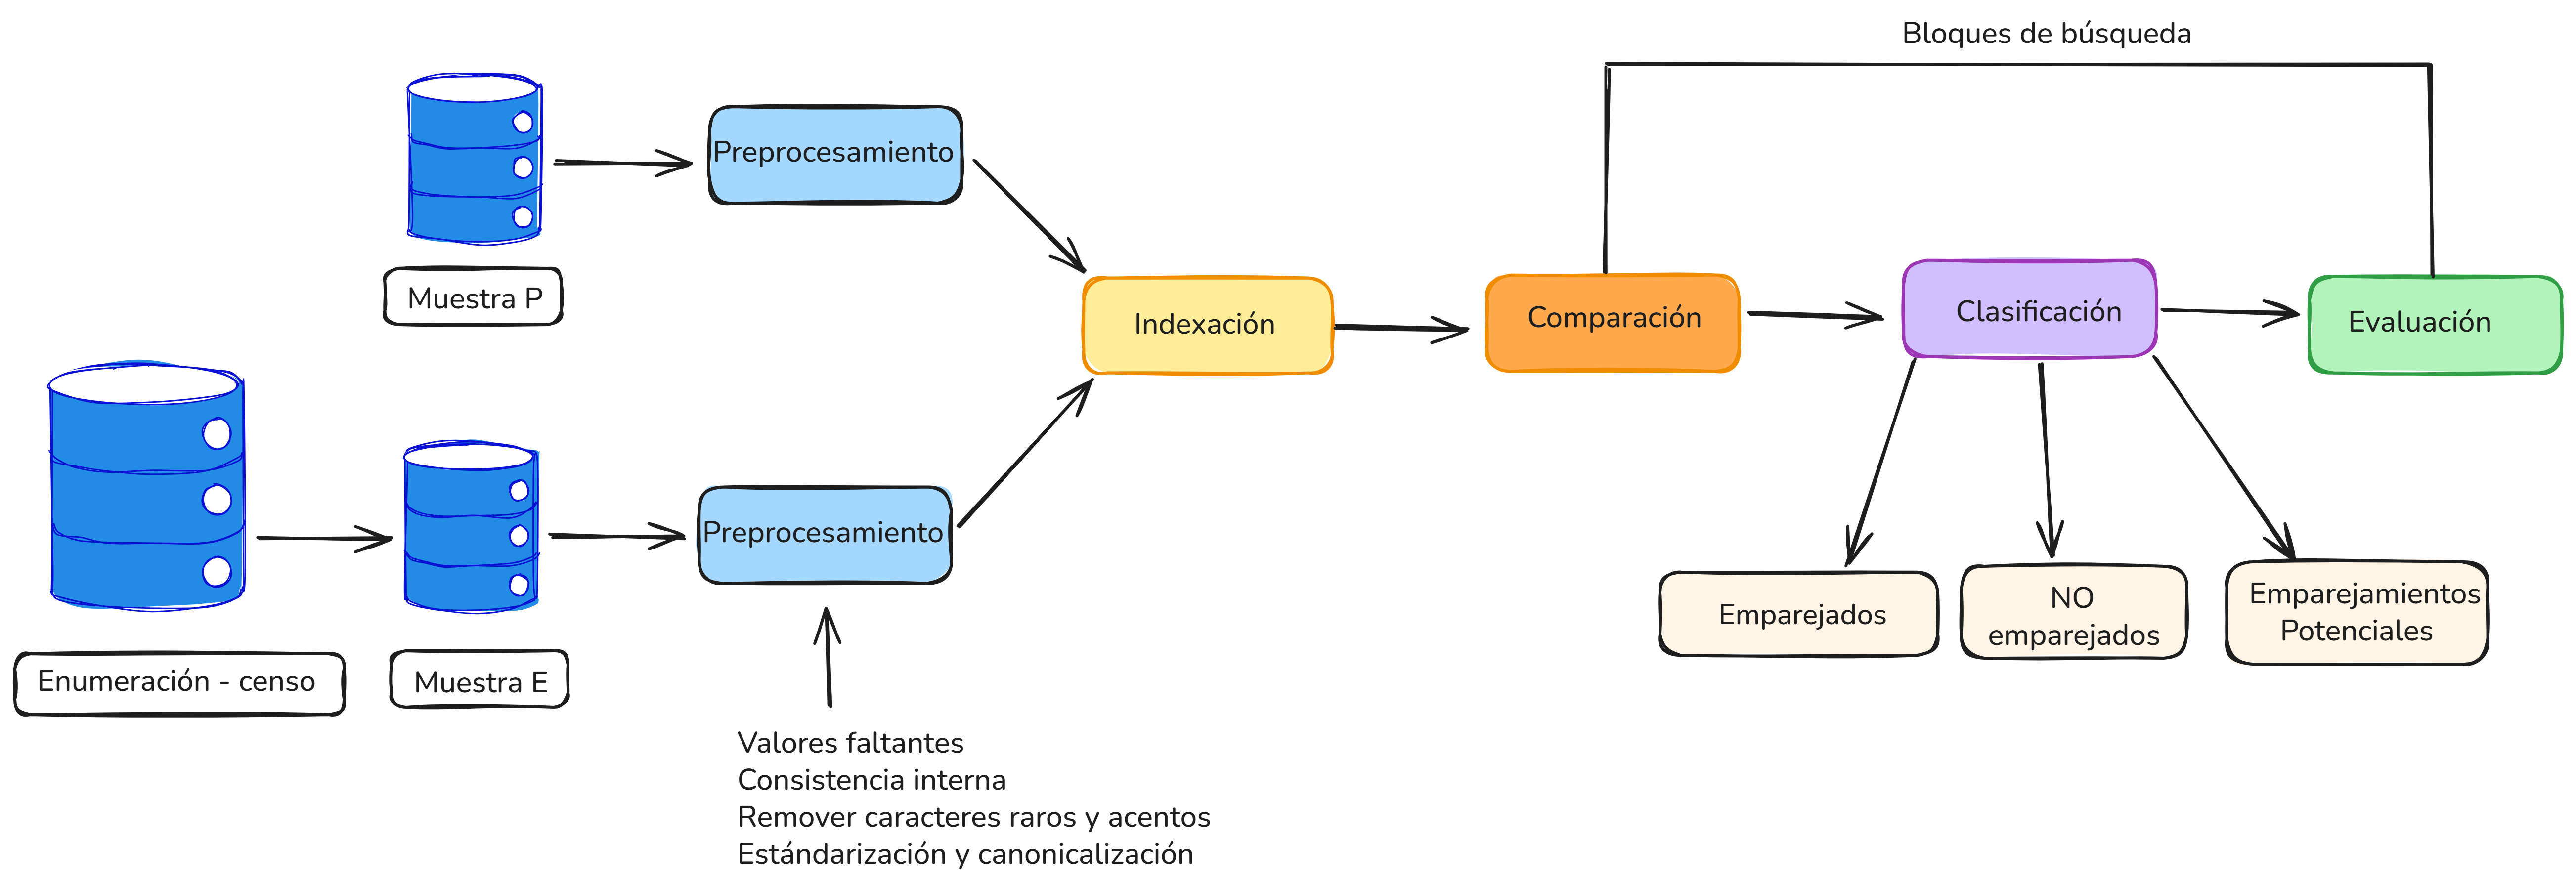
\includegraphics[width=1\linewidth]{images/FlujoMatch} 

}

\caption{Flujo general del proceso de emparejamiento en la PES}\label{fig:match}
\end{figure}

Para los registros que tienen estado ``no emparejado'' se amplia el área de búsqueda hasta llegar al nivel nacional. Como las probabilidades de error de emparejamiento se incrementan cuando se aumenta el área de búsqueda, es recomendable que se haga una revisión clerical de estos registros luego de ser emparejados, incluso si su probabilidad es alta.

Si no hay coincidencia tras ampliar el área de búsqueda, el caso se clasifica como omisión, es decir, personas que no estuvieron enumeradas en el censo.

\section{Flujo general del procedimiento}\label{flujo-general-del-procedimiento}

La Figura \ref{fig:match1q} muestra el flujograma que se debría seguir para realizar este proceso.

\begin{figure}

{\centering 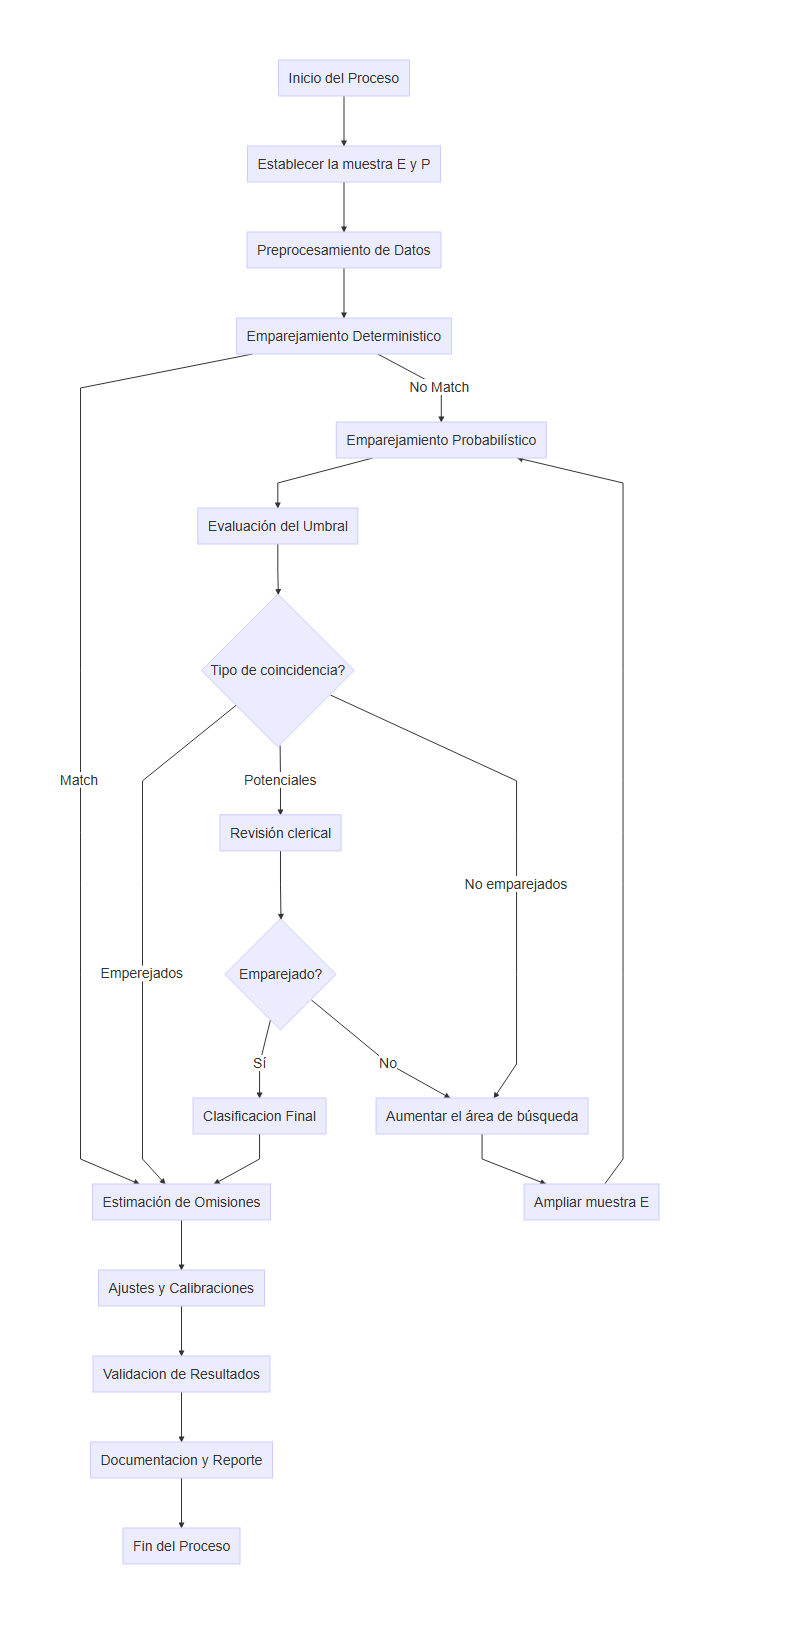
\includegraphics[width=1\linewidth]{images/grafo} 

}

\caption{Flujo general del proceso de emparejamiento en la PES}\label{fig:match1q}
\end{figure}

\chapter{Emparejamiento probabilístico}\label{emparejamiento-probabiluxedstico}

Las bases de datos censales, rara vez se cuentan con identificadores únicos fiables y completos. Esto hace que el emparejamiento exacto basado en igualdad absoluta de valores en atributos clave, como el número de identificación, sea insuficiente. Además, las variaciones en nombres, errores tipográficos, diferencias de formato y registros incompletos son frecuentes.

Por ejemplo, los registros:

\begin{itemize}
\tightlist
\item
  \emph{Nohora Rodriguez, nacida el 8/10/1960}
\item
  \emph{Nora Rodrigues, nacida el 19601008}
\end{itemize}

pueden referirse a la misma persona, pero un algoritmo exacto no emparejará estos registros. por el contrario, el enfoque probabilístico permite capturar estas coincidencias aproximadas mediante modelos estadísticos, como el propuesto por Fellegi y Sunter \citep{fellegi1969theory}.

El emparejamiento probabilístico de registros, también conocido como \emph{record linkage}, tiene una historia extensa en el campo de la estadística y es una técnica fundamental en el contexto de los censos y las encuestas de cobertura. Su objetivo es identificar registros que se refieren a la misma entidad\footnote{Una entidad puede ser un hogar, una persona, una empresa u otro tipo de unidad registrada.} entre diferentes fuentes de datos, incluso cuando no se cuenta con un identificador único o cuando los datos contienen errores, inconsistencias o formatos distintos.

La primera vez que se introdujo formalmente el término \emph{record linkage} fue en el año 1946, para construir un ``libro de vida'' a nivel de individuo, desde el nacimiento hasta la muerte, incluyendo eventos relevantes como matrimonios, divorcios, registros médicos y de seguridad social \citep{dunn1946}. Esta visión anticipaba muchos de los principios de lo que hoy se conoce como integración de datos longitudinales, fundamentales para la planificación de servicios públicos y la mejora de la calidad de las estadísticas nacionales.

Durante las décadas de 1950 y 1960, el avance tecnológico permitió que se comenzara con la automatización del proceso de vinculación de registros. Además, se introdujo el enfoque probabilístico, en el cual se asignan pesos de acuerdo con los atributos comparados, considerando la frecuencia relativa de los valores \citep[\citet{newcombe1962}]{newcombe1959}. Este enfoque sentó las bases para el desarrollo del modelo probabilístico propuesto formalmente por Fellegi y Sunter en 1969, quienes demostraron que bajo ciertas condiciones, es posible derivar una regla óptima para decidir si dos registros corresponden a la misma entidad \citep{fellegi1969theory}.

A lo largo de las décadas siguientes, este marco teórico fue ampliado por William Winkler en el U.S. Census Bureau, incorporando funciones de comparación aproximada de cadenas, ponderaciones basadas en frecuencia y algoritmos como EM para mejorar la estimación de parámetros del modelo de vinculación probabilística \citep[\citet{winkler2006overview}]{winkler1990}. En el contexto de los censos de población y vivienda, estas técnicas han sido fundamentales para evaluar la omisión censal mediante encuestas de cobertura, al comparar registros del censo con los de la encuesta y estimar la omisión neta de forma robusta.

La necesidad de vincular datos de múltiples fuentes ha crecido en paralelo con el aumento en la cantidad de información recolectada por Oficinas Nacionales de Estadística (ONE). En este contexto, el emparejamiento de registros cumple múltiples funciones:

\begin{itemize}
\tightlist
\item
  \textbf{Mejorar la calidad de los datos}, al eliminar duplicados y enriquecer registros incompletos.
\item
  \textbf{Optimizar los costos} de operaciones estadísticas al reutilizar datos existentes. Un caso práctico es el Censo Combinado 2023 de Uruguay.
\item
  \textbf{Viabilizar el análisis longitudinal y de múltiples fuentes}, especialmente en contextos censales donde los datos se recolectan en por intervalos de tiempo \citep{bleiholder2009data}.
\end{itemize}

El proceso de emparejamiento consta generalmente de cinco etapas principales:

\begin{enumerate}
\def\labelenumi{\arabic{enumi}.}
\tightlist
\item
  \textbf{Normalización y preprocesamiento}: limpieza, estandarización y codificación de atributos.
\item
  \textbf{Reducción del espacio de búsqueda}: indexación o bloques
\item
  \textbf{Comparación de registros}: evaluación de similitudes en atributos comunes (nombre, sexo, fecha de nacimiento, dirección).
\item
  \textbf{Clasificación}: asignación de un estado de emparejado (match), no emparejado (non-match) o revisión clerical (posible match), usualmente mediante reglas probabilísticas \citep{fellegi1969theory}.
\item
  \textbf{Predicción final}: umbral de clasificación y validación.
\end{enumerate}

El emparejamiento completo entre dos bases con \(n\) y \(m\) registros implica comparar hasta \(n \times m\) pares, lo que resulta en complejidad cuadrática. Para mitigar este costo, se emplean técnicas de indexación conocidas como \emph{bloqueo o blocking}, que reducen el espacio de comparación considerando solo subconjuntos plausibles de registros.

Una dificultad adicional en el emparejamiento probabilístico es la falta de verdad conocida como \emph{ground truth}, esto ocurre cuando no se dispone de datos que indiquen con certeza si dos registros corresponden a la misma persona. Esto obliga a realizar revisiones clericales para evaluar la calidad de los emparejamientos. Por esta razón, los procesos logísticos de la encuesta de postcensal (PES) deben considerar una fase de sensibilización para que la población esté dispuesta a colaborar y a entregar información fiable, debido a la resistencia que pueden tener porque fueron censadas hace poco tiempo.

El emparejamiento de registros frecuentemente involucra información sensible como nombres, direcciones y fechas de nacimiento. Por tanto, la privacidad y confidencialidad deben ser cuidadosamente protegidas. En particular, cuando el emparejamiento ocurre entre bases de diferentes entidades, en estos casos se deben aplicar las técnicas de emparejamiento preservando la privacidad (PPRL) \citep{christen2023privacy, Vatsalan2020}. Estas consideraciones son especialmente importantes en contextos censales y gubernamentales, donde los datos personales son confidenciales por ley.

\section{Geolocalización}\label{geolocalizaciuxf3n}

El primer paso consiste en geocodificar las direcciones proporcionadas por los encuestados y verificar que las mismas coinciden con los segmentos cartográficos seleccionados. En caso de que algunas direcciones no tengan una precisión a nivel de segmento cartográfico, entonces será necesaria una revisión clerical para verificar las direcciones proporcionadas por los encuestados.

El paquete \texttt{tidygeocoder} \citep{tidygeocoder} puede ser útil para esa tarea, a continuación se presenta un ejemplo de juguete con cinco (5) direcciones en el departamento de Chuquisaca, Bolivia.

\begin{Shaded}
\begin{Highlighting}[]
\FunctionTok{library}\NormalTok{(pacman)}

\FunctionTok{p\_load}\NormalTok{(dplyr, tidygeocoder)}

\NormalTok{datos }\OtherTok{\textless{}{-}} \FunctionTok{tribble}\NormalTok{(}
  \SpecialCharTok{\textasciitilde{}}\NormalTok{DIRECCION, }\SpecialCharTok{\textasciitilde{}}\NormalTok{MUNICIPIO,}
  \StringTok{"Av. Jaime Mendoza 123"}\NormalTok{, }\StringTok{"Sucre"}\NormalTok{,}
  \StringTok{"Calle Bolívar 456"}\NormalTok{, }\StringTok{"Monteagudo"}\NormalTok{,}
  \StringTok{"Plaza 25 de Mayo 789"}\NormalTok{, }\StringTok{"Camargo"}\NormalTok{,}
  \StringTok{"Av. del Maestro 321"}\NormalTok{, }\StringTok{"Villa Serrano"}\NormalTok{,}
  \StringTok{"Calle Potosí 654"}\NormalTok{, }\StringTok{"Zudáñez"}
\NormalTok{)}

\NormalTok{datos }\SpecialCharTok{|\textgreater{}}
  \FunctionTok{mutate}\NormalTok{(}\AttributeTok{addrs =} \FunctionTok{paste0}\NormalTok{(DIRECCION, }\StringTok{", "}\NormalTok{, MUNICIPIO, }\StringTok{", Bolivia"}\NormalTok{)) }\SpecialCharTok{|\textgreater{}}
  \FunctionTok{geocode}\NormalTok{(addrs, }\AttributeTok{method =} \StringTok{"arcgis"}\NormalTok{)}
\end{Highlighting}
\end{Shaded}

\begin{verbatim}
## # A tibble: 5 x 5
##   DIRECCION             MUNICIPIO     addrs                            lat  long
##   <chr>                 <chr>         <chr>                          <dbl> <dbl>
## 1 Av. Jaime Mendoza 123 Sucre         Av. Jaime Mendoza 123, Sucre,~ -19.0 -65.3
## 2 Calle Bolívar 456     Monteagudo    Calle Bolívar 456, Monteagudo~ -19.8 -64.0
## 3 Plaza 25 de Mayo 789  Camargo       Plaza 25 de Mayo 789, Camargo~ -18.0 -62.7
## 4 Av. del Maestro 321   Villa Serrano Av. del Maestro 321, Villa Se~ -19.1 -64.3
## 5 Calle Potosí 654      Zudáñez       Calle Potosí 654, Zudáñez, Bo~ -19.0 -64.8
\end{verbatim}

En caso de que algunos de los puntos de longitud y latitud no queden dentro de los segmentos de la muestra P, los revisores clericales deben verificar las direcciones y establecer si hay descritos algunos puntos de referencia que no se usaron durante el procesamiento automatizado que hubiera afectado la precisión del proceso automático. Los resultados de la geocodificación se utilizan durante el proceso de emparejamiento para identificar áreas de búsqueda alrededor de la dirección proporcionada por el encuestado.

Durante el proceso de geocodificación manual, los revisores asignan una coordenada que permita una mayor precisión. Si no es posible lograr una precisión que apunte a una UPM específica de la muestra P, entonces la misma podrá asociarse a más de una UPM para crear áreas de búsqueda que abarquen dicha dirección. Asimismo, es recomendable que se asigne un código que refleje el nivel de confianza que el revisor manual considera que hay en que la dirección se encuentra dentro del área de búsqueda.

Es recomendable que el emparejamiento automático de personas incluya los geocódigos asignados a las direcciones proporcionadas por los encuestados, así como los nombres, apellidos, la edad, el sexo, el día y mes de nacimiento. Otra información que puede ser usada en el proceso son: los números de teléfono de los encuestados del hogar, datos geográficos como el departamento, municipio o código del segmento. Con este propósito se puede usar un modelo de vinculación probabilística de registros conocido como \emph{record linkage}.

Con el objetivo de examinar la completitud de los nombres, es recomendable que el nombre o apellido se considere suficiente cuando la combinación del primer y segundo nombre, así como la combinación de los apellidos, tengan al menos dos caracteres cada uno. Posteriormente, los revisores clericales deben analizar todos los registros marcados como insuficientes y actualizar los nombres cuando sea posible. Por ejemplo, puede haberse registrado el primer nombre de un niño pero no su apellido, el revisor clerical podrá completar el apellido basándose en el de los padres cuando el parentesco sea determinado. En estos casos, se podrá cambiar el estado de insuficiente a suficiente.

Al finalizar este procesamiento, cada persona de la muestra P y cada persona de la muestra E deben ser codificadas como coincidencia, posible coincidencia, duplicado, posible duplicado o sin coincidencia, y al finalizar la revisión clerical, se usarán los vínculos asignados a las personas de la muestra P y muestra E como insumos para estimar la cobertura neta de la población y sus componentes.

\section{Flujo general}\label{flujo-general}

La Figura \ref{fig:match1} muestra los pasos principales del proceso de emparejamiento. El primer paso es el preprocesamiento de datos, cuyo objetivo es asegurar que los datos de ambas fuentes estén en un formato uniforme y comparable.

El segundo paso se conoce como indexación, acá se busca reducir la complejidad cuadrática del proceso de emparejamiento mediante el uso de estructuras de datos que permiten generar de manera eficiente y efectiva pares de registros candidatos que probablemente correspondan a la misma persona.

En el tercer paso, se realiza la comparación de pares de registros, donde los pares candidatos generados a partir de la indexación se comparan utilizando varias variables.

En el paso de clasificación, los pares de registros se asignan a una de tres categorías: emparejados, no emparejados y emparejamientos potenciales. Si los pares se clasifican como emparejamientos potenciales, se requiere una revisión clerical manual para decidir su estado final (emparejado o no emparejado). En el paso final, se analiza la calidad y la completitud de los datos emparejados.

Para la deduplicación de una única base de datos, todos los pasos del proceso de vinculación siguen siendo aplicables. El preprocesamiento es esencial para asegurar que la base completa esté estandarizada, especialmente si los registros han sido ingresados en diferentes momentos, lo que puede haber introducido variaciones en los formatos o en los métodos de captura de datos. La etapa de indexación también es crítica en la deduplicación, ya que comparar cada registro con todos los demás implica un alto costo computacional.

\begin{figure}

{\centering 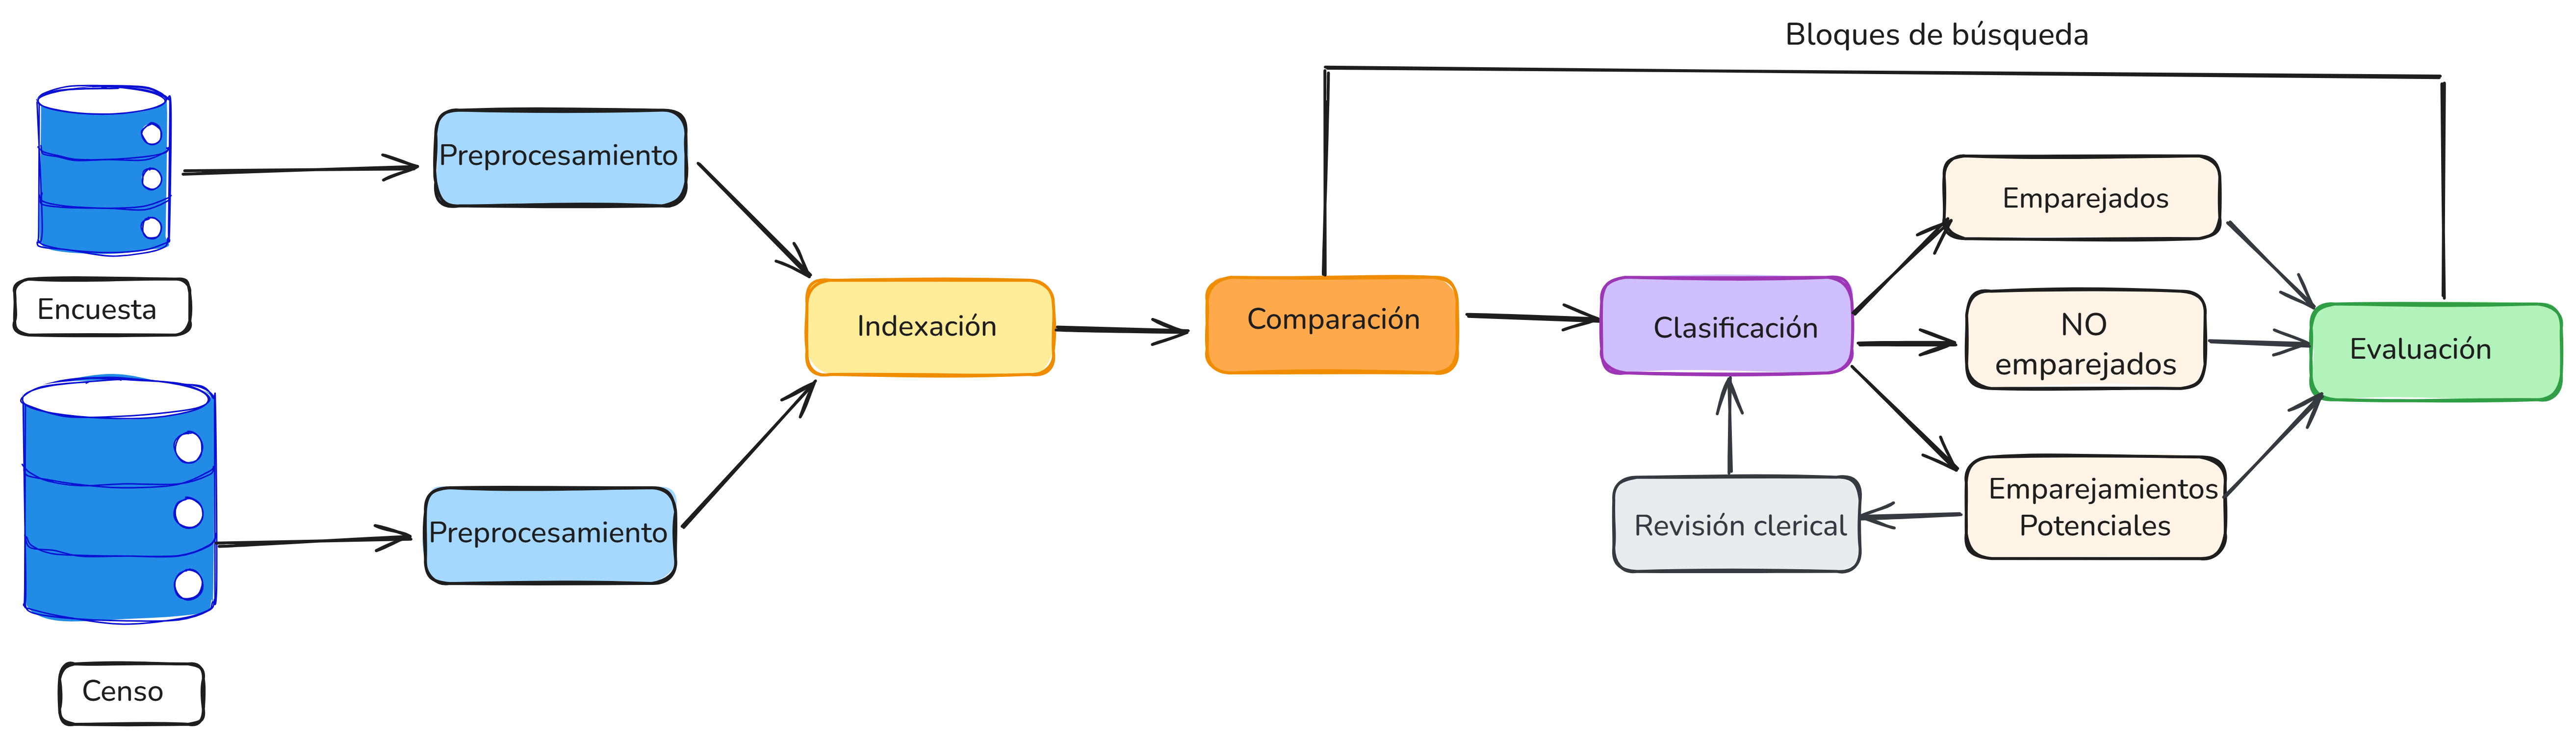
\includegraphics[width=1\linewidth]{images/FlujoMatch2} 

}

\caption{Flujo general del proceso de emparejamiento}\label{fig:match1}
\end{figure}

Para ilustrar las tareas involucradas a lo largo del proceso de emparejamiento de registros, se utilizará un ejemplo compuesto por dos tablas de datos artificiales.

\begin{Shaded}
\begin{Highlighting}[]
\FunctionTok{load}\NormalTok{(}\StringTok{"data/censo.rda"}\NormalTok{)}
\FunctionTok{load}\NormalTok{(}\StringTok{"data/encuesta.rda"}\NormalTok{)}
\end{Highlighting}
\end{Shaded}

A continuación se presenta la estructura para los primeros registros de la tabla censo:

\begin{table}[t]
\caption*{
{\fontsize{20}{25}\selectfont  Tabla censo\fontsize{12}{15}\selectfont }
} 
\fontsize{12.0pt}{14.0pt}\selectfont
\begin{tabular*}{\linewidth}{@{\extracolsep{\fill}}rlllllrrrl}
\toprule
id\_segmento & id\_hogar & id\_censo & {\bfseries \cellcolor[HTML]{F9F9F9}{nombre}} & {\bfseries \cellcolor[HTML]{F9F9F9}{apellido}} & {\bfseries \cellcolor[HTML]{F9F9F9}{sexo}} & anio\_nac & mes\_nac & dia\_nac & {\bfseries \cellcolor[HTML]{F9F9F9}{parentesco}} \\ 
\midrule\addlinespace[2.5pt]
101 & H101\_1 & c1 & Carlos & P\\'erez & M & 1947 & 1 & 1 & Jefe \\ 
101 & H101\_1 & c2 & Luc\\'ia & Castro & F & 1975 & 1 & 1 & Hijo/a \\ 
101 & H101\_1 & c3 & Camila & Castro & F & 2012 & 1 & 1 & Hijo/a \\ 
101 & H101\_1 & c4 & Mar\\'ia & Castro & F & 1959 & 1 & 1 & Nieto/a \\ 
102 & H102\_1 & c5 & Jorge & G\\'omez & M & 1954 & 1 & 1 & Jefe \\ 
102 & H102\_1 & c6 & Sof\\'ia & Ram\\'irez & F & 2000 & 1 & 1 & Hijo/a \\ 
\bottomrule
\end{tabular*}
\end{table}

La tabla encuesta presenta la siguiente estructura para los primeros registros:

\begin{table}[t]
\caption*{
{\fontsize{20}{25}\selectfont  Tabla encuesta\fontsize{12}{15}\selectfont }
} 
\fontsize{12.0pt}{14.0pt}\selectfont
\begin{tabular*}{\linewidth}{@{\extracolsep{\fill}}rllllrl}
\toprule
id\_segmento & id\_hogar & id\_encuesta & nombre\_completo & {\bfseries \cellcolor[HTML]{F9F9F9}{sexo}} & fecha\_nacimiento & {\bfseries \cellcolor[HTML]{F9F9F9}{parentesco}} \\ 
\midrule\addlinespace[2.5pt]
101 & H101\_1 & e1 & Mar\\'ia Castro & F & 1959-1-1 & Nieto/a \\ 
101 & H101\_1 & e2 & Carlos P\\'erez & M & 1947-1-1 & Jefe \\ 
101 & H101\_1 & e3 & Luc\\'ia Castro & F & 1975-1-1 & Hijo/a \\ 
101 & H101\_10 & e4 & Camila Ram\\'irez & F & 2010-1-1 & Hijo/a \\ 
101 & H101\_2 & e5 & Sof\\'i\\'a C\\'astro & F & 1966-1-1 & Jefe \\ 
101 & H101\_2 & e6 & Ana Mart\\'inez & F & 1973-1-1 & C\\'onyuge \\ 
\bottomrule
\end{tabular*}
\end{table}

El objetivo es realizar un proceso de emparejamiento de las dos tablas anteriores. Como puede observarse, aunque ambas contienen información sobre nombre, apellido, sexo, fecha de nacimiento, parentesco y barrio, la estructura de las dos tablas es diferente, al igual que el formato de los valores almacenados en algunas de ellas.

\section{Preprocesamiento}\label{preprocesamiento}

Es común que las tablas de datos que se usarán en el proceso de emparejamiento de datos puedan variar en formato, estructura y contenido. Dado que el emparejamiento de datos comúnmente se basa en información personal, como nombres, sexo, direcciones y fechas de nacimiento, es importante asegurarse de que los datos provenientes de diferentes bases de datos sean limpiados y estandarizados adecuadamente.

El objetivo de esta etapa es garantizar que los atributos utilizados para el emparejamiento tengan la misma estructura y que su contenido siga los mismos formatos. Se ha reconocido que la limpieza y estandarización de datos son pasos cruciales para un emparejamiento exitoso \citep{herzog2007data}. Los datos brutos de entrada deben convertirse en formatos bien definidos y consistentes, y las inconsistencias en la forma en que se representa y codifica la información deben resolverse \citep{churches2002preparation}.

Existen al menos cinco pasos que son necesarios (aunque probablemente no suficientes) en el preprocesamiento de datos:

\begin{enumerate}
\def\labelenumi{\arabic{enumi}.}
\item
  Eliminar caracteres y palabras irrelevantes: Este paso corresponde a una limpieza inicial, donde se eliminan caracteres como comas, dos puntos, puntos y comas, puntos, numerales y comillas. En ciertas aplicaciones, también se pueden eliminar algunas palabras si se sabe que no contienen información relevante para el proceso de emparejamiento. Estas palabras también se conocen como ``stop words'' o palabras vacías.
\item
  Expandir abreviaturas y corregir errores ortográficos: Este segundo paso del preprocesamiento es crucial para mejorar la calidad de los datos a emparejar. Comúnmente, este paso se basa en tablas de búsqueda que contienen variaciones de nombres, apodos, errores ortográficos comunes y sus versiones correctas o expandidas. La estandarización de valores realizada en este paso reducirá significativamente las variaciones en atributos que contienen nombres.
\item
  Codificación fonética: Es muy común que se tengan errores de ortografía o que los nombres se escriban de manera diferente, por ejemplo ``Catalina Benavides'' puede corresponder a ``Katalina Venavidez'', pero un algoritmo no encontrará la coincidencia perfecta, así que lograr el emparejamiento automático se convierte en un desafío.
\item
  Segmentación: Dividir el contenido de atributos que contienen varias piezas de información en un conjunto de nuevos atributos, cada uno con una pieza de información bien definida regularmente es exitoso. El proceso de segmentar valores de atributos también se llama \emph{parsing} \citep{herzog2007data}. Es de gran importancia realizarlo para nombres, direcciones o fechas. Se han desarrollado diversas técnicas para lograr esta segmentación, ya sea utilizando sistemas basados en reglas o técnicas probabilísticas como modelos ocultos de Markov \citep{churches2002preparation}.
\item
  Verificar: Este paso puede aplicarse cuando existen fuentes externas que permiten realizar una validación de los datos, por ejemplo, si se dispone de una base de datos externa que contenga todas las direcciones conocidas y válidas en un país o región. La información detallada en dicha base de datos debe incluir el rango de números de calles, así como combinaciones de nombres de calles para validar la información del censo y de la PES.
\end{enumerate}

\subsection{Limpieza de los datos}\label{limpieza-de-los-datos}

En este paso implementamos una función que nos permita remover los caracteres raros y así limpiar el texto, esta función se ha denominado \texttt{limpiar\_texto()} y en cada línea hemos documentado el objetivo, es importante señalar que pueden existir otras estructuras que pueden ser removidas.

\begin{Shaded}
\begin{Highlighting}[]
\FunctionTok{library}\NormalTok{(pacman)}
\FunctionTok{p\_load}\NormalTok{(dplyr, tidyr, stringr, stringi, assertr)}

\NormalTok{limpiar\_texto }\OtherTok{\textless{}{-}} \ControlFlowTok{function}\NormalTok{(x) \{}
\NormalTok{  x }\SpecialCharTok{|\textgreater{}} 
    \FunctionTok{iconv}\NormalTok{(}\AttributeTok{from =} \StringTok{""}\NormalTok{, }\AttributeTok{to =} \StringTok{"UTF{-}8"}\NormalTok{, }\AttributeTok{sub =} \StringTok{""}\NormalTok{) }\SpecialCharTok{|\textgreater{}} 
    \FunctionTok{str\_to\_lower}\NormalTok{() }\SpecialCharTok{|\textgreater{}}                            \CommentTok{\# Convertir a minúsculas}
    \FunctionTok{stri\_trans\_general}\NormalTok{(}\StringTok{"Latin{-}ASCII"}\NormalTok{) }\SpecialCharTok{|\textgreater{}}         \CommentTok{\# Quitar acentos}
    \FunctionTok{str\_replace\_all}\NormalTok{(}\StringTok{"[[:punct:]]"}\NormalTok{, }\StringTok{" "}\NormalTok{) }\SpecialCharTok{|\textgreater{}}       \CommentTok{\# Quitar puntuación}
    \FunctionTok{str\_replace\_all}\NormalTok{(}\StringTok{"}\SpecialCharTok{\textbackslash{}\textbackslash{}}\StringTok{s+"}\NormalTok{, }\StringTok{" "}\NormalTok{) }\SpecialCharTok{|\textgreater{}}              \CommentTok{\# Espacios múltiples}
    \FunctionTok{str\_trim}\NormalTok{()                                   }\CommentTok{\# Quitar espacios extremos}
\NormalTok{\}}
\end{Highlighting}
\end{Shaded}

De igual manera el investigador puede establecer un vector de palabras vacías o irrelevantes, que prefiere eliminar de las cadena de texto. Por ejemplo, a continuación se crea el vector \texttt{stop\_words} con varias palabras y se aplica la función \texttt{eliminar\_stopwords()} para eliminarlas.

\begin{Shaded}
\begin{Highlighting}[]
\NormalTok{stop\_words }\OtherTok{\textless{}{-}} \FunctionTok{c}\NormalTok{(}\StringTok{"de"}\NormalTok{, }\StringTok{"del"}\NormalTok{, }\StringTok{"la"}\NormalTok{, }\StringTok{"los"}\NormalTok{, }\StringTok{"las"}\NormalTok{, }\StringTok{"el"}\NormalTok{, }\StringTok{"y"}\NormalTok{)}

\NormalTok{eliminar\_stopwords }\OtherTok{\textless{}{-}} \ControlFlowTok{function}\NormalTok{(x, }\AttributeTok{palabras =}\NormalTok{ stop\_words) \{}
\NormalTok{  palabras\_pattern }\OtherTok{\textless{}{-}} \FunctionTok{paste0}\NormalTok{(}\StringTok{"}\SpecialCharTok{\textbackslash{}\textbackslash{}}\StringTok{b("}\NormalTok{, }\FunctionTok{paste}\NormalTok{(palabras, }\AttributeTok{collapse =} \StringTok{"|"}\NormalTok{), }\StringTok{")}\SpecialCharTok{\textbackslash{}\textbackslash{}}\StringTok{b"}\NormalTok{)}
  \FunctionTok{str\_remove\_all}\NormalTok{(x, palabras\_pattern) }\SpecialCharTok{\%\textgreater{}\%}
    \FunctionTok{str\_replace\_all}\NormalTok{(}\StringTok{"}\SpecialCharTok{\textbackslash{}\textbackslash{}}\StringTok{s+"}\NormalTok{, }\StringTok{" "}\NormalTok{) }\SpecialCharTok{\%\textgreater{}\%}
    \FunctionTok{str\_trim}\NormalTok{()}
\NormalTok{\}}
\end{Highlighting}
\end{Shaded}

Ahora podemos aplicar nuestras funciones sobre las variables de interés en los conjuntos de datos. Es importante destacar que el proceso de preprocesamiento de datos no debe sobrescribir los datos originales y en su lugar, se deben crear nuevos atributos que contengan los datos limpios y estandarizados, o generar nuevas tablas de datos que contengan los datos limpios y estandarizados.

\begin{Shaded}
\begin{Highlighting}[]
\NormalTok{censo\_limpio }\OtherTok{\textless{}{-}}\NormalTok{ censo }\SpecialCharTok{|\textgreater{}} 
                \FunctionTok{mutate}\NormalTok{(}\FunctionTok{across}\NormalTok{(}\FunctionTok{c}\NormalTok{(nombre, apellido, parentesco, sexo),}
                              \SpecialCharTok{\textasciitilde{}}\FunctionTok{eliminar\_stopwords}\NormalTok{(}\FunctionTok{limpiar\_texto}\NormalTok{(.))))}
\end{Highlighting}
\end{Shaded}

\begin{table}[t]
\caption*{
{\fontsize{20}{25}\selectfont  Tabla censo\_limpio\fontsize{12}{15}\selectfont }
} 
\fontsize{12.0pt}{14.0pt}\selectfont
\begin{tabular*}{\linewidth}{@{\extracolsep{\fill}}rlllllrrrl}
\toprule
id\_segmento & id\_hogar & id\_censo & {\bfseries \cellcolor[HTML]{F9F9F9}{nombre}} & {\bfseries \cellcolor[HTML]{F9F9F9}{apellido}} & {\bfseries \cellcolor[HTML]{F9F9F9}{sexo}} & anio\_nac & mes\_nac & dia\_nac & {\bfseries \cellcolor[HTML]{F9F9F9}{parentesco}} \\ 
\midrule\addlinespace[2.5pt]
101 & H101\_1 & c1 & carlos & perez & m & 1947 & 1 & 1 & jefe \\ 
101 & H101\_1 & c2 & lucia & castro & f & 1975 & 1 & 1 & hijo a \\ 
101 & H101\_1 & c3 & camila & castro & f & 2012 & 1 & 1 & hijo a \\ 
101 & H101\_1 & c4 & maria & castro & f & 1959 & 1 & 1 & nieto a \\ 
102 & H102\_1 & c5 & jorge & gomez & m & 1954 & 1 & 1 & jefe \\ 
102 & H102\_1 & c6 & sofia & ramirez & f & 2000 & 1 & 1 & hijo a \\ 
\bottomrule
\end{tabular*}
\end{table}

En el caso de la tabla de la encuesta, primero se separa el nombre\_completo en varias variables para generar la misma estructura que la tabla del censo, o podría unirse las variables del censo para generar un nombre\_unico, lo importante es dejar las tablas en la misma estructura. De igual forma para la fecha de nacimiento. Paso seguido se aplican las funciones sobre las variables de interés.

\begin{Shaded}
\begin{Highlighting}[]
\NormalTok{encuesta\_limpia }\OtherTok{\textless{}{-}}\NormalTok{ encuesta }\SpecialCharTok{|\textgreater{}} 
                   \FunctionTok{separate}\NormalTok{(nombre\_completo, }\FunctionTok{c}\NormalTok{(}\StringTok{"nombre"}\NormalTok{, }\StringTok{"apellido"}\NormalTok{), }\AttributeTok{sep=}\StringTok{" "}\NormalTok{) }\SpecialCharTok{|\textgreater{}} 
                   \FunctionTok{separate}\NormalTok{(fecha\_nacimiento, }\FunctionTok{c}\NormalTok{(}\StringTok{"anio\_nac"}\NormalTok{, }\StringTok{"mes\_nac"}\NormalTok{, }\StringTok{"dia\_nac"}\NormalTok{), }\AttributeTok{sep=}\StringTok{"{-}"}\NormalTok{) }\SpecialCharTok{|\textgreater{}} 
                   \FunctionTok{mutate}\NormalTok{(}\FunctionTok{across}\NormalTok{(}\FunctionTok{c}\NormalTok{(}\StringTok{"anio\_nac"}\NormalTok{, }\StringTok{"mes\_nac"}\NormalTok{, }\StringTok{"dia\_nac"}\NormalTok{), }\SpecialCharTok{\textasciitilde{}}\FunctionTok{as.numeric}\NormalTok{(.))) }\SpecialCharTok{|\textgreater{}}   
                   \FunctionTok{mutate}\NormalTok{(}\FunctionTok{across}\NormalTok{(}\FunctionTok{c}\NormalTok{(nombre, apellido, parentesco, sexo),}
                                 \SpecialCharTok{\textasciitilde{}}\FunctionTok{eliminar\_stopwords}\NormalTok{(}\FunctionTok{limpiar\_texto}\NormalTok{(.))))}
\end{Highlighting}
\end{Shaded}

\begin{table}[t]
\caption*{
{\fontsize{20}{25}\selectfont  Tabla encuesta\_limpia\fontsize{12}{15}\selectfont }
} 
\fontsize{12.0pt}{14.0pt}\selectfont
\begin{tabular*}{\linewidth}{@{\extracolsep{\fill}}rlllllrrrl}
\toprule
id\_segmento & id\_hogar & id\_encuesta & {\bfseries \cellcolor[HTML]{F9F9F9}{nombre}} & {\bfseries \cellcolor[HTML]{F9F9F9}{apellido}} & {\bfseries \cellcolor[HTML]{F9F9F9}{sexo}} & anio\_nac & mes\_nac & dia\_nac & {\bfseries \cellcolor[HTML]{F9F9F9}{parentesco}} \\ 
\midrule\addlinespace[2.5pt]
101 & H101\_1 & e1 & maria & castro & f & 1959 & 1 & 1 & nieto a \\ 
101 & H101\_1 & e2 & carlos & perez & m & 1947 & 1 & 1 & jefe \\ 
101 & H101\_1 & e3 & lucia & castro & f & 1975 & 1 & 1 & hijo a \\ 
101 & H101\_10 & e4 & camila & ramirez & f & 2010 & 1 & 1 & hijo a \\ 
101 & H101\_2 & e5 & sofia & castro & f & 1966 & 1 & 1 & jefe \\ 
101 & H101\_2 & e6 & ana & martinez & f & 1973 & 1 & 1 & conyuge \\ 
\bottomrule
\end{tabular*}
\end{table}

Las versiones preprocesadas (limpiadas y estandarizadas) de las dos tablas de datos ahora tienen los mismos atributos. El formato y contenido de estos atributos han sido estandarizados.

\subsection{Codificación fonética}\label{codificaciuxf3n-fonuxe9tica}

Existen diversas funciones diseñadas para codificar fonéticamente los valores de ciertos atributos antes de utilizarlos en procesos de emparejamiento o deduplicación de registros. Su propósito es mitigar los errores derivados de variaciones en la escritura o errores ortográficos, especialmente en variables como nombres, apellidos u otras susceptibles a inconsistencias tipográficas. Estas funciones buscan agrupar cadenas de texto que suenan de forma similar al ser pronunciadas, aunque estén escritas de manera distinta.

La codificación fonética también puede combinarse con medidas de similitud como la distancia de Levenshtein, Smith-Waterman o el coeficiente de Jaccard, para comparar cadenas de texto que suenan de forma similar \citep{navarro2001guided, nauman2022introduction}.

El principio fundamental consiste en transformar un texto en un código fonético basado en su pronunciación. ESin embargo, muchas de las técnicas clásicas fueron desarrolladas para el idioma inglés, lo que limita su aplicabilidad directa en contextos de América Latina y el Caribe, donde se emplean otros idiomas como el español, portugués, francés o lenguas indígenas.

A pesar de estas limitaciones, algunos métodos pueden resultar útiles en este contexto. Por ejemplo, el algoritmo Double Metaphone permite generar codificaciones alternativas para un mismo nombre, considerando distintas variantes ortográficas. Su uso puede mejorar la identificación de coincidencias en registros provenientes de censos y encuestas, donde la calidad y la estandarización de los nombres pueden variar significativamente entre fuentes y regiones.

\subsubsection{Algoritmo Soundex}\label{algoritmo-soundex}

El algoritmo Soundex es uno de los métodos más antiguos y ampliamente conocidos para la codificación fonética de cadenas de texto. Fue desarrollado originalmente por \citep{odell1918soundex} y ha sido utilizado tradicionalmente en tareas como la consolidación de listas de nombres y la indexación de registros. En el ámbito del emparejamiento de registros entre censos y encuestas de cobertura en América Latina y el Caribe, Soundex puede servir como una herramienta complementaria para enfrentar errores de escritura, diferencias dialectales, y variaciones ortográficas en nombres y apellidos.

Soundex fue diseñado originalmente para nombres en inglés estadounidense, por lo que puede presentar limitaciones en su aplicación directa a nombres hispanos, portugueses o de otras lenguas de la región. Sin embargo, su simplicidad y bajo costo computacional lo convierten en un buen punto de partida para ilustrar los principios básicos de codificación fonética.

\begin{longtable}[]{@{}ll@{}}
\toprule\noalign{}
Letras & Código \\
\midrule\noalign{}
\endhead
\bottomrule\noalign{}
\endlastfoot
b, f, p, v & 1 \\
c, g, j, k, q, s, x, z & 2 \\
d, t & 3 \\
l & 4 \\
m, n & 5 \\
r & 6 \\
a, e, i, o, u, h, w, y & 0 (se elimina) \\
\end{longtable}

Después de convertir la cadena en dígitos, se eliminan todos los ceros (que corresponden a vocales y las letras \emph{`h', `w'} e \emph{`y'}), así como las repeticiones del mismo número. Por ejemplo:

Las reglas del algoritmo son:

\begin{itemize}
\tightlist
\item
  Conservar la primera letra del nombre.
\item
  Convertir las letras restantes en números usando la tabla de codificación.
\item
  Eliminar los ceros, ya que las vocales y ciertas consonantes no aportan a la diferenciación fonética.
\item
  Eliminar repeticiones consecutivas del mismo número (por ejemplo, ``bb'' se convierte en ``b1'', no en ``b11'').
\item
  Si el código resultante tiene más de tres dígitos, se trunca para que tenga una longitud final de cuatro caracteres (letra + tres dígitos).
\item
  Si tiene menos de tres dígitos, se rellena con ceros.
\end{itemize}

La siguiente tabla presenta un ejemplo de codificación con el algoritmo soundex. Se observa que, a pesar de que algunos nombres suenan igual, el algoritmo los diferencia según la primera letra.

\begin{longtable}[]{@{}lll@{}}
\toprule\noalign{}
Nombre & Codificación & Resultado Final \\
\midrule\noalign{}
\endhead
\bottomrule\noalign{}
\endlastfoot
Catalina & C, 0, 3, 4, 0, 4, 5, 0 & C345 \\
Katalina & K, 0, 3, 4, 0, 4, 5, 0 & K345 \\
Yovana & Y, 0, 1, 5, 0, 0 & Y150 \\
Jovanna & J, 0, 1, 5, 5, 0, 0 & J150 \\
Giovanna & G, 0, 1, 5, 5, 0, 0 & G150 \\
Yenny & Y, 0, 5, 5, 0 & Y550 → Y500 \\
Yeni & Y, 0, 5, 0 & Y50 → Y500 \\
Gonzales & G, 0, 5, 2, 4, 2 & G524 \\
Gonzalez & G, 0, 5, 2, 4, 2 & G524 \\
\end{longtable}

El algoritmo se puede implementar en R con el paquete \texttt{phonics} \citep{howard2020phonetic} de la siguiente manera

\begin{Shaded}
\begin{Highlighting}[]
\FunctionTok{library}\NormalTok{(pacman)}
\FunctionTok{p\_load}\NormalTok{(phonics)}

\NormalTok{nombres }\OtherTok{\textless{}{-}} \FunctionTok{c}\NormalTok{(}\StringTok{"Catalina"}\NormalTok{, }\StringTok{"Katalina"}\NormalTok{, }\StringTok{"Yovana"}\NormalTok{, }\StringTok{"Jovanna"}\NormalTok{, }\StringTok{"Giovanna"}\NormalTok{, }\StringTok{"Yenny"}\NormalTok{, }\StringTok{"Yeni"}\NormalTok{, }\StringTok{"Gonzalez"}\NormalTok{, }\StringTok{"Gonzales"}\NormalTok{)}

\NormalTok{codigos\_soundex }\OtherTok{\textless{}{-}} \FunctionTok{soundex}\NormalTok{(}\FunctionTok{limpiar\_texto}\NormalTok{(nombres))  }

\FunctionTok{names}\NormalTok{(codigos\_soundex) }\OtherTok{\textless{}{-}}\NormalTok{ nombres}
\NormalTok{codigos\_soundex}
\end{Highlighting}
\end{Shaded}

\begin{verbatim}
## Catalina Katalina   Yovana  Jovanna Giovanna    Yenny     Yeni Gonzalez 
##   "C345"   "K345"   "Y150"   "J150"   "G150"   "Y500"   "Y500"   "G524" 
## Gonzales 
##   "G524"
\end{verbatim}

\subsection{Metaphone}\label{metaphone}

El algoritmo Metaphone es una técnica de codificación fonética desarrollada por Lawrence Philips en 1990 \citep{philips1990hanging}, diseñada para mejorar la coincidencia de palabras con escritura diferente pero pronunciación similar. A diferencia de algoritmos como Soundex, Metaphone no se limita al análisis de nombres en inglés, lo que lo convierte en una alternativa útil para la deduplicación de datos en contextos de otros idiomas, como los encontrados en los censos y encuestas de cobertura en América Latina y el Caribe.

Una ventaja clave de Metaphone es que no asigna códigos numéricos sino representaciones fonéticas alfabéticas, lo que permite una mayor precisión fonética, especialmente para consonantes. El algoritmo captura 16 sonidos consonánticos comunes en múltiples idiomas y los representa en la transcripción resultante.

No obstante, como fue diseñado originalmente para el inglés, su aplicación en nombres de origen hispano o indígena puede ser limitada. Para superar estas limitaciones, se desarrollaron algoritmos posteriores como Double Metaphone, que permite hasta dos codificaciones por palabra para capturar variaciones fonéticas adicionales, especialmente útiles en bases de datos que tienen varios idiomas \citep{christen2012data}.

El algoritmo se puede implementar en R con el paquete \texttt{phonics} de la siguiente manera:

\begin{Shaded}
\begin{Highlighting}[]
\NormalTok{codigos\_metaphone }\OtherTok{\textless{}{-}} \FunctionTok{metaphone}\NormalTok{(}\FunctionTok{limpiar\_texto}\NormalTok{(nombres))}

\FunctionTok{names}\NormalTok{(codigos\_metaphone) }\OtherTok{\textless{}{-}}\NormalTok{ nombres}
\NormalTok{codigos\_metaphone}
\end{Highlighting}
\end{Shaded}

\begin{verbatim}
## Catalina Katalina   Yovana  Jovanna Giovanna    Yenny     Yeni Gonzalez 
##   "KTLN"   "KTLN"    "YFN"    "JFN"    "JFN"     "YN"     "YN"  "KNSLS" 
## Gonzales 
##  "KNSLS"
\end{verbatim}

Note que este algoritmo resulta más preciso para los nombres y apellidos de nuestro ejemplo, generando la misma codificación para los nombres que suenan igual.

\subsection{Algoritmo Statistics Canada}\label{algoritmo-statistics-canada}

El algoritmo fonético desarrollado por Statistics Canada, también conocido como el método de Lynch y Arends \citep{lynch1977selection}, es una alternativa simple y eficiente para la codificación fonética de nombres, ampliamente utilizada en censos y procesos de vinculación de registros administrativos en Canadá.

Este método es útil cuando se requiere una solución rápida, pero con capacidad de captura de errores comunes de transcripción y ortografía. Es especialmente relevante en contextos de censos de población y encuestas de gran escala en países de América Latina y el Caribe, donde los nombres pueden tener múltiples variantes fonéticas y ortográficas debido a la diversidad cultural.

Entre las características principales del algoritmo se encuentran:

\begin{enumerate}
\def\labelenumi{\arabic{enumi}.}
\tightlist
\item
  Elimina las vocales, conservando únicamente la estructura consonántica de los nombres.
\item
  Reduce sonidos duplicados, unificando repeticiones que suelen aparecer por errores de tipeo o escritura fonética.
\item
  No recodifica letras individuales, lo que disminuye la carga computacional.
\item
  Proporciona una forma simplificada de agrupación fonética que no depende del idioma, a diferencia de algoritmos como Soundex o Metaphone.
\end{enumerate}

\begin{Shaded}
\begin{Highlighting}[]
\NormalTok{codigos\_statcan }\OtherTok{\textless{}{-}} \FunctionTok{statcan}\NormalTok{(}\FunctionTok{limpiar\_texto}\NormalTok{(nombres))}

\FunctionTok{names}\NormalTok{(codigos\_statcan) }\OtherTok{\textless{}{-}}\NormalTok{ nombres}
\NormalTok{codigos\_statcan}
\end{Highlighting}
\end{Shaded}

\begin{verbatim}
## Catalina Katalina   Yovana  Jovanna Giovanna    Yenny     Yeni Gonzalez 
##   "CTLN"   "KTLN"    "YVN"    "JVN"    "GVN"     "YN"     "YN"   "GNZL" 
## Gonzales 
##   "GNZL"
\end{verbatim}

Hay otras alternativas que pueden ser utilizadas, en \citet{howard2020phonetic} se pueden encontrar otros algoritmos como NYSIIS, Caverphone, Cologne, RogerRoot, Phonex o MRA.

\subsection{Adaptación para Encuestas de América Latina}\label{adaptaciuxf3n-para-encuestas-de-amuxe9rica-latina}

A diferencia de los algoritmos fonéticos clásicos como Soundex, Metaphone y StatCan, que fueron desarrollados principalmente para nombres de origen anglosajón, en América Latina los nombres presentan una gran diversidad fonética y ortográfica influenciada por lenguas indígenas, castellano, portugués y otras tradiciones europeas. Por ello, se ha desarrollado un algoritmo personalizado que tiene en cuenta las transformaciones fonéticas y ortográficas más comunes en la región.

La función \texttt{codif\_fonetico()} fue diseñada por los autores de este material para capturar las variantes más frecuentes en los nombres latinoamericanos, mediante las siguientes transformaciones:

\begin{enumerate}
\def\labelenumi{\arabic{enumi}.}
\tightlist
\item
  Reducción de dobles letras y sílabas características: ll → y, qu → k, ch → x.
\item
  Conversión de combinaciones como ce, ci a se, si; y gue, gui a gi.
\item
  Reglas específicas como \^{}j → y, \^{}hua → wa, y \^{}hu → w, comunes en nombres quechuas o aimaras.
\item
  Normalización de acentos, letra ñ y otros caracteres mediante stri\_trans\_general(\ldots, ``Latin-ASCII'').
\item
  Eliminación de vocales y letras mudas para capturar la estructura fonética esencial.
\item
  Conversión de v a b, y de z a s, fonéticamente indistinguibles en la mayoría de los dialectos del español latino.
\end{enumerate}

El orden en que se aplican las transformaciones también juega un rol especial, el usuario puede ampliar las reglas si así lo desea, incorporando nuevas líneas.

\begin{Shaded}
\begin{Highlighting}[]
\FunctionTok{require}\NormalTok{(stringi)}
\FunctionTok{require}\NormalTok{(stringr)}

\NormalTok{codif\_fonetico }\OtherTok{\textless{}{-}} \ControlFlowTok{function}\NormalTok{(nombre) \{}
\NormalTok{  nombre }\OtherTok{\textless{}{-}} \FunctionTok{tolower}\NormalTok{(nombre)}
\NormalTok{  nombre }\OtherTok{\textless{}{-}} \FunctionTok{gsub}\NormalTok{(}\StringTok{"lly"}\NormalTok{, }\StringTok{"li"}\NormalTok{, nombre)}
\NormalTok{  nombre }\OtherTok{\textless{}{-}} \FunctionTok{gsub}\NormalTok{(}\StringTok{"ll"}\NormalTok{, }\StringTok{"y"}\NormalTok{, nombre)}
\NormalTok{  nombre }\OtherTok{\textless{}{-}} \FunctionTok{gsub}\NormalTok{(}\StringTok{"yn$"}\NormalTok{, }\StringTok{"in"}\NormalTok{, nombre)}
\NormalTok{  nombre }\OtherTok{\textless{}{-}} \FunctionTok{gsub}\NormalTok{(}\StringTok{"\^{}hu"}\NormalTok{, }\StringTok{"w"}\NormalTok{, nombre) }
\NormalTok{  nombre }\OtherTok{\textless{}{-}} \FunctionTok{gsub}\NormalTok{(}\StringTok{"\^{}hua"}\NormalTok{, }\StringTok{"wa"}\NormalTok{, nombre)}
\NormalTok{  nombre }\OtherTok{\textless{}{-}} \FunctionTok{gsub}\NormalTok{(}\StringTok{"\^{}qui|\^{}qhi"}\NormalTok{, }\StringTok{"ki"}\NormalTok{, nombre)}
\NormalTok{  nombre }\OtherTok{\textless{}{-}} \FunctionTok{gsub}\NormalTok{(}\StringTok{"\^{}xi"}\NormalTok{, }\StringTok{"ji"}\NormalTok{, nombre)}
\NormalTok{  nombre }\OtherTok{\textless{}{-}} \FunctionTok{gsub}\NormalTok{(}\StringTok{"\^{}j"}\NormalTok{, }\StringTok{"y"}\NormalTok{, nombre) }
\NormalTok{  nombre }\OtherTok{\textless{}{-}} \FunctionTok{gsub}\NormalTok{(}\StringTok{"\^{}gio"}\NormalTok{, }\StringTok{"yo"}\NormalTok{, nombre)}
\NormalTok{  nombre }\OtherTok{\textless{}{-}} \FunctionTok{gsub}\NormalTok{(}\StringTok{"y$"}\NormalTok{, }\StringTok{"i"}\NormalTok{, nombre) }
\NormalTok{  nombre }\OtherTok{\textless{}{-}} \FunctionTok{gsub}\NormalTok{(}\StringTok{"}\SpecialCharTok{\textbackslash{}\textbackslash{}}\StringTok{b(}\SpecialCharTok{\textbackslash{}\textbackslash{}}\StringTok{w*)hui(}\SpecialCharTok{\textbackslash{}\textbackslash{}}\StringTok{w*)}\SpecialCharTok{\textbackslash{}\textbackslash{}}\StringTok{b"}\NormalTok{, }\StringTok{"}\SpecialCharTok{\textbackslash{}\textbackslash{}}\StringTok{1wi}\SpecialCharTok{\textbackslash{}\textbackslash{}}\StringTok{2"}\NormalTok{, nombre)}
\NormalTok{  nombre }\OtherTok{\textless{}{-}} \FunctionTok{gsub}\NormalTok{(}\StringTok{"ch"}\NormalTok{, }\StringTok{"x"}\NormalTok{, nombre)}
\NormalTok{  nombre }\OtherTok{\textless{}{-}} \FunctionTok{gsub}\NormalTok{(}\StringTok{"[aeiouh]"}\NormalTok{, }\StringTok{""}\NormalTok{, nombre)}
\NormalTok{  nombre }\OtherTok{\textless{}{-}} \FunctionTok{gsub}\NormalTok{(}\StringTok{"v"}\NormalTok{, }\StringTok{"b"}\NormalTok{, nombre)}
\NormalTok{  nombre }\OtherTok{\textless{}{-}} \FunctionTok{gsub}\NormalTok{(}\StringTok{"z"}\NormalTok{, }\StringTok{"s"}\NormalTok{, nombre)}
\NormalTok{  nombre }\OtherTok{\textless{}{-}} \FunctionTok{str\_replace\_all}\NormalTok{(nombre, }\StringTok{"c(?=[ei])"}\NormalTok{, }\StringTok{"s"}\NormalTok{)  }
\NormalTok{  nombre }\OtherTok{\textless{}{-}} \FunctionTok{gsub}\NormalTok{(}\StringTok{"c"}\NormalTok{, }\StringTok{"k"}\NormalTok{, nombre)          }
\NormalTok{  nombre }\OtherTok{\textless{}{-}} \FunctionTok{gsub}\NormalTok{(}\StringTok{"qu"}\NormalTok{, }\StringTok{"k"}\NormalTok{, nombre)}
\NormalTok{  nombre }\OtherTok{\textless{}{-}} \FunctionTok{str\_replace\_all}\NormalTok{(nombre, }\StringTok{"g(?=[ei])"}\NormalTok{, }\StringTok{"j"}\NormalTok{)}
\NormalTok{  nombre }\OtherTok{\textless{}{-}} \FunctionTok{gsub}\NormalTok{(}\StringTok{"gue|gui"}\NormalTok{, }\StringTok{"gi"}\NormalTok{, nombre)}
\NormalTok{  nombre }\OtherTok{\textless{}{-}} \FunctionTok{stri\_trans\_general}\NormalTok{(nombre, }\StringTok{"Latin{-}ASCII"}\NormalTok{)  }
\NormalTok{  nombre }\OtherTok{\textless{}{-}} \FunctionTok{gsub}\NormalTok{(}\StringTok{"(.)}\SpecialCharTok{\textbackslash{}\textbackslash{}}\StringTok{1+"}\NormalTok{, }\StringTok{"}\SpecialCharTok{\textbackslash{}\textbackslash{}}\StringTok{1"}\NormalTok{, nombre)  }
\NormalTok{  nombre }\OtherTok{\textless{}{-}} \FunctionTok{gsub}\NormalTok{(}\StringTok{"[aeiou]"}\NormalTok{, }\StringTok{""}\NormalTok{, nombre)}
  
  \FunctionTok{toupper}\NormalTok{(nombre)}
\NormalTok{\}}
\end{Highlighting}
\end{Shaded}

A continuación se presenta la aplicación para nuestro ejemplo

\begin{Shaded}
\begin{Highlighting}[]
\NormalTok{datos }\OtherTok{\textless{}{-}} \FunctionTok{data.frame}\NormalTok{(}\AttributeTok{nombre =}\NormalTok{ nombres) }\SpecialCharTok{|\textgreater{}} 
         \FunctionTok{mutate}\NormalTok{(}\AttributeTok{nombre =} \FunctionTok{limpiar\_texto}\NormalTok{(nombre)) }\SpecialCharTok{|\textgreater{}} 
         \FunctionTok{mutate}\NormalTok{(}\AttributeTok{codif =} \FunctionTok{codif\_fonetico}\NormalTok{(nombre))}
\end{Highlighting}
\end{Shaded}

\begin{table}[t]
\fontsize{12.0pt}{14.0pt}\selectfont
\begin{tabular*}{\linewidth}{@{\extracolsep{\fill}}ll}
\toprule
{\bfseries \cellcolor[HTML]{F9F9F9}{nombre}} & {\bfseries \cellcolor[HTML]{F9F9F9}{codif}} \\ 
\midrule\addlinespace[2.5pt]
catalina & KTLN \\ 
katalina & KTLN \\ 
yovana & YBN \\ 
jovanna & YBN \\ 
giovanna & YBN \\ 
yenny & YN \\ 
yeni & YN \\ 
gonzalez & GNSLS \\ 
gonzales & GNSLS \\ 
\bottomrule
\end{tabular*}
\end{table}

Considere otro ejemplo. La siguiente tabla presenta el resultado de aplicar los algoritmos fonéticos al campo del nombre. En este caso, se puede observar que el método propuesto, columna \emph{nom\_latino}, origina un mejor resultado que los otros algoritmos.

\begin{Shaded}
\begin{Highlighting}[]
\NormalTok{nom }\OtherTok{\textless{}{-}}\NormalTok{ df }\SpecialCharTok{|\textgreater{}} 
       \FunctionTok{mutate}\NormalTok{(}\AttributeTok{soundex =}\FunctionTok{soundex}\NormalTok{(}\FunctionTok{limpiar\_texto}\NormalTok{(nombre)),}
              \AttributeTok{metaphone =} \FunctionTok{metaphone}\NormalTok{(}\FunctionTok{limpiar\_texto}\NormalTok{(nombre)),}
              \AttributeTok{statcan =} \FunctionTok{statcan}\NormalTok{(}\FunctionTok{limpiar\_texto}\NormalTok{(nombre)),}
              \AttributeTok{latino =} \FunctionTok{codif\_fonetico}\NormalTok{(}\FunctionTok{limpiar\_texto}\NormalTok{(nombre)))}
\end{Highlighting}
\end{Shaded}

\begin{table}[t]
\fontsize{12.0pt}{14.0pt}\selectfont
\begin{tabular*}{\linewidth}{@{\extracolsep{\fill}}llllll}
\toprule
{\bfseries \cellcolor[HTML]{F9F9F9}{nombre}} & {\bfseries \cellcolor[HTML]{F9F9F9}{apellido}} & {\bfseries \cellcolor[HTML]{F9F9F9}{soundex}} & {\bfseries \cellcolor[HTML]{F9F9F9}{metaphone}} & {\bfseries \cellcolor[HTML]{F9F9F9}{statcan}} & {\bfseries \cellcolor[HTML]{F9F9F9}{latino}} \\ 
\midrule\addlinespace[2.5pt]
Wilmer & Huanca & W456 & WLMR & WLMR & WLMR \\ 
Guilmer & Wuanca & G456 & KLMR & GLMR & GLMR \\ 
Wilmar & Guanca & W456 & WLMR & WLMR & WLMR \\ 
Yohana & Kuispe & Y500 & YHN & YHN & YN \\ 
Johanna & Quispe & J500 & JHN & JHN & YN \\ 
Bryan & Kispe & B650 & BRYN & BRN & BRYN \\ 
Brayan & Qhispe & B650 & BRYN & BRN & BRYN \\ 
Marleni & Rodriguez & M645 & MRLN & MRLN & MRLN \\ 
Marleny & Rodrigues & M645 & MRLN & MRLN & MRLN \\ 
Marlenni & Rodriwues & M645 & MRLN & MRLN & MRLN \\ 
Nely & \~Nahui & N400 & NL & NL & NL \\ 
Neli & Nahui & N400 & NL & NL & NL \\ 
Nelly & Nahuy & N400 & NL & NL & NL \\ 
Ximena & \~Nawi & X550 & SMN & XMN & YMN \\ 
Jimena & \~Nahui & J550 & JMN & JMN & YMN \\ 
\bottomrule
\end{tabular*}
\end{table}

En el caso del apellido, es fundamental tener en cuenta las particularidades culturales de cada región, ya que pueden influir significativamente en la forma en que son escritos o pronunciados. Estas variaciones hacen que ningún algoritmo de codificación fonética sea completamente robusto por sí solo, por lo que es recomendable adaptar o complementar los métodos según el contexto local.

\begin{Shaded}
\begin{Highlighting}[]
\NormalTok{apell }\OtherTok{\textless{}{-}}\NormalTok{ df }\SpecialCharTok{|\textgreater{}} 
         \FunctionTok{mutate}\NormalTok{(}\AttributeTok{soundex =}\FunctionTok{soundex}\NormalTok{(}\FunctionTok{limpiar\_texto}\NormalTok{(apellido)),}
                \AttributeTok{metaphone =} \FunctionTok{metaphone}\NormalTok{(}\FunctionTok{limpiar\_texto}\NormalTok{(apellido)),}
                \AttributeTok{statcan =} \FunctionTok{statcan}\NormalTok{(}\FunctionTok{limpiar\_texto}\NormalTok{(apellido)),}
                \AttributeTok{latino =} \FunctionTok{codif\_fonetico}\NormalTok{(}\FunctionTok{limpiar\_texto}\NormalTok{(apellido)))}
\end{Highlighting}
\end{Shaded}

\begin{table}[t]
\fontsize{12.0pt}{14.0pt}\selectfont
\begin{tabular*}{\linewidth}{@{\extracolsep{\fill}}llllll}
\toprule
{\bfseries \cellcolor[HTML]{F9F9F9}{nombre}} & {\bfseries \cellcolor[HTML]{F9F9F9}{apellido}} & {\bfseries \cellcolor[HTML]{F9F9F9}{soundex}} & {\bfseries \cellcolor[HTML]{F9F9F9}{metaphone}} & {\bfseries \cellcolor[HTML]{F9F9F9}{statcan}} & {\bfseries \cellcolor[HTML]{F9F9F9}{latino}} \\ 
\midrule\addlinespace[2.5pt]
Wilmer & Huanca & H520 & HNK & HNC & WNK \\ 
Guilmer & Wuanca & W520 & WNK & WNC & WNK \\ 
Wilmar & Guanca & G520 & KNK & GNC & GNK \\ 
Yohana & Kuispe & K210 & KSP & KSP & KSP \\ 
Johanna & Quispe & Q210 & KSP & QSP & KSP \\ 
Bryan & Kispe & K210 & KSP & KSP & KSP \\ 
Brayan & Qhispe & Q210 & KHSP & QHSP & KSP \\ 
Marleni & Rodriguez & R362 & RTRKS & RDRG & RDRGS \\ 
Marleny & Rodrigues & R362 & RTRKS & RDRG & RDRGS \\ 
Marlenni & Rodriwues & R362 & RTRWS & RDRW & RDRWS \\ 
Nely & \~Nahui & N000 & NH & NH & NW \\ 
Neli & Nahui & N000 & NH & NH & NW \\ 
Nelly & Nahuy & N000 & NH & NH & NW \\ 
Ximena & \~Nawi & N000 & NW & NW & NW \\ 
Jimena & \~Nahui & N000 & NH & NH & NW \\ 
\bottomrule
\end{tabular*}
\end{table}

La siguiente tabla muestra el resultado de aplicar la función \texttt{codif\_fonetico} tanto al nombre como al apellido. No obstante, se recomienda utilizar en cada campo el algoritmo fonético que mejor se adapte a las características lingüísticas y culturales del caso específico.

\begin{Shaded}
\begin{Highlighting}[]
\NormalTok{res }\OtherTok{\textless{}{-}}\NormalTok{ df }\SpecialCharTok{|\textgreater{}} 
         \FunctionTok{mutate}\NormalTok{(}\AttributeTok{nom\_cod =} \FunctionTok{codif\_fonetico}\NormalTok{(}\FunctionTok{limpiar\_texto}\NormalTok{(nombre)),}
                \AttributeTok{ape\_cod =} \FunctionTok{codif\_fonetico}\NormalTok{(}\FunctionTok{limpiar\_texto}\NormalTok{(apellido)))}
\end{Highlighting}
\end{Shaded}

\begin{table}[t]
\fontsize{12.0pt}{14.0pt}\selectfont
\begin{tabular*}{\linewidth}{@{\extracolsep{\fill}}llll}
\toprule
{\bfseries \cellcolor[HTML]{F9F9F9}{nombre}} & {\bfseries \cellcolor[HTML]{F9F9F9}{apellido}} & nom\_cod & ape\_cod \\ 
\midrule\addlinespace[2.5pt]
Wilmer & Huanca & WLMR & WNK \\ 
Guilmer & Wuanca & GLMR & WNK \\ 
Wilmar & Guanca & WLMR & GNK \\ 
Yohana & Kuispe & YN & KSP \\ 
Johanna & Quispe & YN & KSP \\ 
Bryan & Kispe & BRYN & KSP \\ 
Brayan & Qhispe & BRYN & KSP \\ 
Marleni & Rodriguez & MRLN & RDRGS \\ 
Marleny & Rodrigues & MRLN & RDRGS \\ 
Marlenni & Rodriwues & MRLN & RDRWS \\ 
Nely & \~Nahui & NL & NW \\ 
Neli & Nahui & NL & NW \\ 
Nelly & Nahuy & NL & NW \\ 
Ximena & \~Nawi & YMN & NW \\ 
Jimena & \~Nahui & YMN & NW \\ 
\bottomrule
\end{tabular*}
\end{table}

Ahora aplicaremos la función \texttt{codif\_fonetico} a nuestros conjuntos de datos del censo y de la encuesta

\begin{Shaded}
\begin{Highlighting}[]
\NormalTok{censo\_limpio }\OtherTok{\textless{}{-}}\NormalTok{ censo\_limpio }\SpecialCharTok{|\textgreater{}} 
                \FunctionTok{mutate}\NormalTok{(}\FunctionTok{across}\NormalTok{(}\FunctionTok{c}\NormalTok{(nombre, apellido), }\SpecialCharTok{\textasciitilde{}}\FunctionTok{codif\_fonetico}\NormalTok{(.), }\AttributeTok{.names =} \StringTok{"\{.col\}\_cod"}\NormalTok{))}

\NormalTok{encuesta\_limpia }\OtherTok{\textless{}{-}}\NormalTok{ encuesta\_limpia }\SpecialCharTok{|\textgreater{}} 
                   \FunctionTok{mutate}\NormalTok{(}\FunctionTok{across}\NormalTok{(}\FunctionTok{c}\NormalTok{(nombre, apellido), }\SpecialCharTok{\textasciitilde{}}\FunctionTok{codif\_fonetico}\NormalTok{(.), }\AttributeTok{.names =} \StringTok{"\{.col\}\_cod"}\NormalTok{))}
\end{Highlighting}
\end{Shaded}

\section{Indexación}\label{indexaciuxf3n}

Las tablas de datos limpias y estandarizadas están listas para ser emparejadas. Inicialmente, cada registro de la tabla del censo necesita compararse con todos los registros de la tabla de la encuesta. Esto conduce a un número total de comparaciones de pares de registros que es cuadrático respecto al tamaño de las tablas de datos a emparejar. Por ejemplo, en nuestro ejercicio la tabla del censo tiene 97 registros y la tabla de la encuesta tiene 54 registros, así que sería necesario un total de 5238 comparaciones.

Por supuesto, esta comparación \emph{ingenua} de todos los pares de registros no es escalable para datos muy grandes. Por ejemplo, el censo de Colombia en el año 2018 tuvo una enumeración de más de 44 millones de personas y usó una PES de 283 mil personas, lo que originaría más de 12 billones de comparaciones de pares de registros. Incluso si se pudieran realizar 100 mil comparaciones por segundo, el proceso de comparación tomaría más de 33 mil horas, más de mil días, que equivale a casi 4 años.

Por lo anterior es necesario realizar una optimización del proceso usando técnicas de indexación (blocking) combinado con un proceso de procesamiento en paralelo y de ser posible sistemas distribuidos (como Apache Spark).

En las muestras de cobertura se usan segmentos muestrales equivalentes a los del censo, es decir, el código del segmento se refiere a la misma área geográfica, y en consecuencia es más probable que una persona que vive en el segmento 1 de la muestra de cobertura, también se encuentre en el segmento 1 del censo; así que comparar los pares de registros dentro del mismo segmento será la primera alternativa. Sin embargo, cuando el tiempo entre el censo y la PES empieza a ser mayor, la probabilidad de que las personas se encuentren en el mismo segmento se reduce, esto debido a que las familias se pueden mudar y en ese caso el enfoque de bloqueo pierde el par porque están en segmentos diferentes, esto también ocurre con los moovers o personas que el día del censo no están en su lugar de residencia habitual. Otros ejemplos más complejos pueden darse cuando una mujer se ha casado y cambia su apellido y dirección, y por lo tanto no es detectada por los criterios de bloqueo y tampoco se detectaría en la comparación completa.

En este sentido, del censo se extrae la muestra de enumeración (muestra E) que corresponde a todos los hogares que están en los mismos segmentos de la PES (muestra P), y de esta forma iniciar el proceso de emparejamiento con estos dos conjuntos de datos.

Sea \(n_0\) el tamaño de la muestra de la PES, \(N_{+1}\) la cantidad de personas enumeradas en el censo y \(n_E\) la cantidad de personas enumeradas en la muestra E. Los pasos de la indexación son:

\begin{enumerate}
\def\labelenumi{\arabic{enumi}.}
\tightlist
\item
  Realizar el emparejamiento entre la muestra E y la muestra P. Suponga que \(C^{(1)}\) es el conjunto de personas emparejadas en este paso, donde \(n_1<n_0\) es la cantidad de personas emparejadas, entonces \(P^{(1)}\) es el conjunto de personas de la muestra P que no fueron emparejadas y \(m_1 = n_0 - n_1\) es la cantidad de personas que no fueron emparejadas en este paso.
\item
  Sea \(M^{(2)}\) la muestra de segmentos en un área más grande alrededor de cada segmento de la muestra \(P\), esto para generar los nuevos bloques de indexación, es decir, si el segmento de la muestra \(P\) es una manzana cartográfica entonces el bloque podría ampliarse a una sección cartográfica o barrio para generar una búsqueda en un área mayor pero sin que se desborde la cantidad de comparaciones.
\item
  Sea \(E_2 = M^{(2)} - C^{(1)}\) la muestra de enumeración en un área más grande luego de retirar los elementos que ya fueron emparejados.
\item
  Realizar el emparejamiento entre la muestra \(E_2\) y la muestra \(P^{(1)}\). Suponga que \(C^{(2)}\) es el conjunto de personas emparejadas en este paso, donde \(n_2<m_1\) es la cantidad de personas emparejadas, entonces \(P^{(2)}\) es el conjunto de personas de la muestra \(P^{(1)}\) que no fueron emparejadas y \(m_2 = m_1 - n_2\) es la cantidad de personas que no fueron emparejadas en este paso.
\item
  Sea \(M^{(3)}\) la muestra de segmentos en un área más grande alrededor de cada bloque usado en \(M^{(2)}\), es decir, si en el paso anterior el bloque se amplió a una sección cartográfica entonces ahora se puede ampliar a un sector censal o si era el barrio entonces ampliarlo a una zona catastral más grande, y así generar una búsqueda en un área mayor pero sin que se desborde la cantidad de comparaciones.
\item
  Sea \(E_3 = M^{(3)} - \bigcup_{i=1}^2C^{(i)}\) la muestra de enumeración en un área más grande luego de retirar los elementos que ya fueron emparejados.
\item
  Realizar el emparejamiento entre la muestra \(E_3\) y la muestra \(P^{(2)}\). Ahora \(C^{(3)}\) es el conjunto de personas emparejadas en este paso, donde \(n_3<m_2\) es la cantidad de personas emparejadas, entonces \(P^{(3)}\) es el conjunto de personas de la muestra \(P^{(2)}\) que no fueron emparejadas y \(m_3 = m_2 - n_3\) es la cantidad de personas que no fueron emparejadas en este paso.
\item
  Continuar el procedimiento hasta que \(M^{(j)}\) sea igual al censo o hasta que \(m_j=0\), es decir, que no hay elementos sin emparejar.
\end{enumerate}

\section{Comparación}\label{comparaciuxf3n}

Existen varios métodos para la comparación de cadenas y otros tipos de variables en procesos de emparejamiento de registros. A continuación se describen algunas de las métricas que son más utilizadas, sus fundamentos matemáticos, ventajas, limitaciones y posibles aplicaciones en contextos como nombres de personas, direcciones, fechas, ubicaciones geográficas y otros campos relevantes en bases de datos administrativas.

\subsection{Distancia de Levenshtein}\label{distancia-de-levenshtein}

La distancia de Levenshtein es una métrica que calcula el número mínimo de operaciones de edición (inserciones, eliminaciones y sustituciones) necesarias para transformar una cadena de texto en otra. Sea \(s_1\) y \(s_2\) dos cadenas de texto. Se construye una matriz \(d[i,j]\) tal que:

\[d[i, j] = 
\begin{cases}
d[i - 1, j - 1] & \text{si } s_1[i] = s_2[j] \\
\min \begin{cases}
d[i - 1, j] + 1 \\ 
d[i, j - 1] + 1 \\ 
d[i - 1, j - 1] + 1
\end{cases} & \text{si } s_1[i] \ne s_2[j]
\end{cases}
\]

La distancia de Levenshtein entre \(s_1\) y \(s_2\) es el valor \(d[|s_1|, |s_2|]\). Puede transformarse en una medida de similitud, así:

\[\text{sim}_{\text{levenshtein}}(s_1, s_2) = 1 - \frac{\text{dist}_{\text{levenshtein}}(s_1, s_2)}{\max(|s_1|, |s_2|)}\]

Esta métrica es simétrica con respecto a \(s_1\) y \(s_2\), y satisface la propiedad \(|\ |s_1| - |s_2|\ | \le \text{dist}_{\text{levenshtein}}(s_1, s_2)\) \citep{christen2012data}.

\textbf{Ejemplo}: Suponga que se tienen las cadenas \(s_1 = \texttt{Laura}\) y \(s_2=\texttt{Lara}\). Transformar ``Laura'' en ``Lara'' se debe eliminar la ``u'', es decir que solo se requiere una operación, así que la distancia de Levenshtein es 1. Si tenemos en cuenta que las longitudes de las palabras son \(|s_1|=5\) y \(|s_2|=4\), entonces

\[\text{sim}_{\text{levenshtein}}(s_1, s_2) = 1 - \frac{1}{\max(5, 4)}=1-\frac{1}{5}=0.8\]

\subsection{Comparación de Jaro y Winkler}\label{comparaciuxf3n-de-jaro-y-winkler}

La similitud de Jaro está especialmente diseñada para nombres y toma en cuenta caracteres comunes y transposiciones \citep{christen2012data}:

\[\text{sim}_{\text{jaro}}(s_1, s_2) = \frac{1}{3} \left( \frac{c}{|s_1|} + \frac{c}{|s_2|} + \frac{c - t}{c} \right)\]

donde \(c\) es el número de caracteres coincidentes y \(t\) el número de transposiciones. La similitud de Jaro-Winkler ajusta la de Jaro con base en un prefijo común:

\[\text{sim}_{\text{winkler}}(s_1, s_2) = \text{sim}_{\text{jaro}}(s_1, s_2) + p \cdot (1 - \text{sim}_{\text{jaro}}(s_1, s_2)) \cdot 0.1\]

donde \(p\) es el número de caracteres idénticos al inicio (\(0\leq p \leq 4\)).

\textbf{Ejemplo}: Para las cadenas \(s_1 = \texttt{Laura}\) y \(s_2=\texttt{Lara}\) se tienen 3 caracteres coincidentes (L, a, a), \(c=3\). Además, la segunda ``a'' de ``Laura'' está en posición 5, mientras que en ``Lara'' está en posición 4, esto indica que al menos una letra está fuera de lugar con respecto a su par coincidente y esto se cuenta como una transposición, por lo tanto habrá 1 transposición. Jaro considera las transposiciones como el número de caracteres coincidentes que están en diferente orden entre las dos cadenas, dividido por 2, esto es:

\[t = \frac{\text{Número de caracteres fuera de lugar}}{2} = \frac{1}{2}\]

\[\text{sim}_{\text{jaro}}(\text{Laura}, \text{Lara}) = \frac{1}{3}\left( \frac{3}{5} + \frac{3}{4} + \frac{3 - 1/2}{3}\right) \approx 0.728\]

\subsection{Comparación de fechas y edades}\label{comparaciuxf3n-de-fechas-y-edades}

Las fechas y edades se comparan de forma directa, considerando:

\begin{itemize}
\tightlist
\item
  Diferencia de días, meses o años.
\item
  Rangos aceptables para considerar coincidencias (por ejemplo, diferencias de 1 año en edad).
\item
  En caso de comparar edad y fecha de nacimiento, se puede validar la coherencia temporal.
\end{itemize}

Una forma alternativa de comparar fechas es convertirlas en edades y luego calcular la diferencia en términos porcentuales, lo cual permite cierto grado de tolerancia. Para ello, las edades se deben calcular respecto a una fecha fija, que puede ser la fecha del cierre de la PES o la fecha del emparejamiento entre bases de datos o cualquier fecha relevante al contexto.

Supongamos que \(d_1\) y \(d_2\) representan la edad (en días o años) calculada desde la fecha fija. Entonces, la diferencia porcentual de edad (DPE) se calcula como:

\[\text{dpe} = \frac{|d_1 - d_2|}{\max(d_1, d_2)} \cdot 100.\]

Con base en este valor, se puede calcular la similitud porcentual de edad como:

\[
\text{sim}_{\text{edad_porc}} =
\begin{cases}
1.0 - \frac{\text{dpe}}{\text{dpe}_{\max}}, & \text{si } \text{dpe} < \text{dpe}_{\max} \\
0.0, & \text{en otro caso}
\end{cases}
\]

donde \(\text{dpe}_{\max} \in (0, 100)\) representa la diferencia porcentual máxima tolerada \citep{christen2012data}.

\subsection{Comparación geográfica}\label{comparaciuxf3n-geogruxe1fica}

Para campos geográficos como coordenadas o nombres de lugares se puede usar una distancia euclidiana o geodésica. Por ejemplo, la fórmula de Haversine que es utilizada para calcular la distancia entre dos puntos de una esfera dadas sus coordenadas de longitud y latitud. En caso de tener las coordenadas, se define:

\[d = 2r \cdot \arcsin\left( \sqrt{\sin^2\left(\frac{\phi_2 - \phi_1}{2}\right) + \cos(\phi_1) \cos(\phi_2) \sin^2\left(\frac{\lambda_2 - \lambda_1}{2}\right)} \right)\]

donde \(\phi\) es la latitud, \(\lambda\) la longitud y \(r\) el radio de la Tierra. De igual forma, se puede hacer una comparación desde nivel país hasta nivel barrio (matching jerárquico) o usando la codificación administrativa normalizada (DANE, INEGI, etc.).

\section{Clasificación}\label{clasificaciuxf3n}

El enfoque clásico es el modelo probabilístico de Fellegi y Sunter \citep{fellegi1969theory}, este modelo considera dos conjuntos de registros:

\begin{itemize}
\tightlist
\item
  \(A\): registros provenientes del censo
\item
  \(B\): registros provenientes de la PES
\end{itemize}

El objetivo es determinar si un par \((a, b) \in A \times B\) representa la misma entidad (es decir, un \emph{match}) o no.

Se define el universo total de pares posibles como:

\[A \cup B = M \times U\]

En donde:

\begin{itemize}
\tightlist
\item
  \(M\): conjunto de pares que son emparejamientos
\item
  \(U\): conjunto de pares que no son emparejados
\end{itemize}

Para cada par \((a, b)\) se define una función de comparación:

\[\boldsymbol{\gamma}(a, b) = (\gamma_1, \gamma_2, \dots, \gamma_d) \in \{0,1\}^d\]

En donde \(d\) es el número de atributos comparados (por ejemplo, nombre, sexo, fecha de nacimiento), y cada \(\gamma_j\) indica si hay coincidencia (\(\gamma_j = 1\)) o no (\(\gamma_j = 0\)) en el atributo \(j\).

El modelo asume independencia condicional de las comparaciones dado el estado del emparejamiento (match o non-match). Así, para un vector de comparación específico \(\boldsymbol{g}\), se cumple:

\[P(\boldsymbol{\gamma} = \boldsymbol{g} \mid M) = \prod_{j=1}^d m_j^{g_j} (1 - m_j)^{1 - g_j}\]

y,

\[P(\boldsymbol{\gamma} = \boldsymbol{g} \mid U) = \prod_{j=1}^d u_j^{g_j} (1 - u_j)^{1 - g_j}\]

En donde:
- \(m_j = P(\gamma_j = 1 \mid M)\) es la probabilidad de coincidencia en el atributo \(j\) entre pares que son matches
- \(u_j = P(\gamma_j = 1 \mid U)\) es la probabilidad de coincidencia en el atributo \(j\) entre pares que no son matches

Estos parámetros pueden estimarse mediante métodos de máxima verosimilitud, como el algoritmo EM o mediante enfoques bayesianos \citep{winkler2000using, larsen2001iterative}.

Para decidir si un par \((a, b)\) representa la misma entidad, se calcula la razón de verosimilitud (también llamada \emph{puntaje de coincidencia} o \emph{match score}):

\[\log L(\boldsymbol{g}) = \log P(\boldsymbol{\gamma} = \boldsymbol{g} \mid M) - \log P(\boldsymbol{\gamma} = \boldsymbol{g} \mid U)\]

Este valor representa la evidencia a favor de que el par \((a, b)\) corresponde a un emparejamiento verdadero. Cuanto mayor sea el valor de \(\log L(\boldsymbol{g})\), mayor será la probabilidad de que los registros representen a la misma persona.

Basándose en los valores del puntaje de coincidencia, se definen dos umbrales:

\begin{itemize}
\tightlist
\item
  Si \(\log L(\boldsymbol{g}) \geq T_M\): se clasifica como \emph{emparejado}.
\item
  Si \(\log L(\boldsymbol{g}) \leq T_U\): se clasifica como \emph{no emparejado}.
\item
  Si \(T_U < \log L(\boldsymbol{g}) < T_M\): se clasifica como \emph{emparejamiento potencial}, sujeto a revisión clerical.
\end{itemize}

Este enfoque tradicional puede complementarse con modelos de aprendizaje supervisado o no supervisado. En estos casos, los pares de registros se representan como vectores de características derivadas de la comparación y se utilizan reglas de clasificación que buscan maximizar las coincidencias reales, para más detalles se recomienda consultar \citep[Capítulo 6]{christen2012data}.

\section{Evaluación}\label{evaluaciuxf3n}

Como se ha discutido, las técnicas de clasificación para el emparejamiento de datos buscan maximizar la calidad de los resultados. No obstante, evaluar dicha calidad requiere la existencia de un conjunto de referencia, es decir, un conjunto donde se conozca con certeza si cada par de registros corresponde a la misma entidad o no. Esta información debe reflejar fielmente las características de los datos reales bajo análisis \citep{christen2012data}.

En el contexto de censos y encuestas de cobertura, un emparejamiento correcto implica que un registro del censo y uno de la encuesta representan a la misma persona. De manera análoga, un par no emparejado representa dos entidades distintas. La disponibilidad de datos de referencia permite calcular métricas similares a las usadas en modelos de aprendizaje automático para problemas de clasificación binaria \citep{menestrina2010evaluating}.

En la práctica, estos conjuntos de referencia rara vez están disponibles de forma directa. Por ello, es necesario implementar procesos de codificación manual, que consisten en realizar un muestreo de la muestra P (emparejada) y realizar la verificación manual en la muestra E (o en el censo) para verificar manualmente su veracidad. Este procedimiento puede ser costoso, especialmente si se aplican esquemas de muestreo estratificado que demanden una cantidad significativa de revisiones.

Dado un conjunto de referencia, los pares de registros se clasifican en las siguientes categorías \citep{christen2012data}:

\begin{itemize}
\tightlist
\item
  \textbf{Verdaderos positivos (VP)}: pares correctamente emparejados.\\
\item
  \textbf{Falsos positivos (FP)}: pares que fueron emparejados incorrectamente.\\
\item
  \textbf{Verdaderos negativos (VN)}: pares correctamente no emparejados.\\
\item
  \textbf{Falsos negativos (FN)}: pares que no fueron emparejados, pero deberían haberlo sido.
\end{itemize}

En contextos censales, suele haber un desbalance extremo entre clases. Por esta razón, métricas como la exactitud (\emph{accuracy}) o la especificidad pueden ser engañosas. Por ejemplo, un clasificador que marque todos los pares como ``no emparejados'' puede alcanzar una alta exactitud.

\subsection{Métricas de desempeño}\label{muxe9tricas-de-desempeuxf1o}

Las métricas más informativas en estas operaciones estadísticas son \citep{christen2012data, nauman2022introduction}:

\begin{enumerate}
\def\labelenumi{\arabic{enumi}.}
\item
  \textbf{Precisión} (\emph{Precision}): Proporción de emparejamientos correctos entre los clasificados como positivos.

  \[prec = \frac{VP}{VP + FP}\]
\item
  \textbf{Exhaustividad} (\emph{Recall}): Proporción de emparejamientos reales detectados.

  \[rec = \frac{VP}{VP + FN}\]
\item
  \textbf{Medida-F} (\emph{F-measure}): Media armónica de precisión y exhaustividad.

  \[F_1 = 2 \cdot \frac{P \cdot R}{P + R}\]
\end{enumerate}

\subsection{Métricas de eficiencia}\label{muxe9tricas-de-eficiencia}

Además de la calidad del emparejamiento, se deben evaluar aspectos de eficiencia del proceso:

\begin{itemize}
\tightlist
\item
  \textbf{Reducción}: proporción de pares descartados durante la etapa de indexación o bloqueo.
\item
  \textbf{Completitud de pares}: proporción de emparejamientos verdaderos que fueron efectivamente retenidos después del bloqueo.
\item
  \textbf{Calidad de pares}: proporción de los pares retenidos que son verdaderos emparejamientos.
\end{itemize}

Estas métricas son útiles para comparar algoritmos de indexación y estrategias de bloqueo.

\subsection{Revisión clerical}\label{revisiuxf3n-clerical}

En las operaciones censales, el emparejamiento automático entre la muestra de cobertura y el censo suele ser insuficiente. Por esta razón, es común implementar procesos de revisión manual, conocidas como revisión clerical, que son realizadas por un equipo de expertos, quienes validan los posibles emparejamientos ambiguos o dudosos. La calidad de esta revisión depende de múltiples factores:

\begin{itemize}
\tightlist
\item
  La experiencia y entrenamiento de los revisores.
\item
  La disponibilidad de herramientas que faciliten la comparación contextual de los registros (por ejemplo, mostrando registros similares o agrupando por hogar).
\item
  El acceso a fuentes de información adicionales (como historiales de direcciones, nombres alternativos, o registros administrativos complementarios).
\end{itemize}

En resumen, la evaluación rigurosa del emparejamiento requiere no solo técnicas automáticas robustas, sino también mecanismos de validación y control de calidad que aseguren su confiabilidad.

\section{Implementación}\label{implementaciuxf3n}

A continuación se presenta un resumen de los principales paquetes de R y Python que se pueden utilizar para la vinculación probabilística de registros:

\begin{longtable}[]{@{}
  >{\raggedright\arraybackslash}p{(\linewidth - 4\tabcolsep) * \real{0.0709}}
  >{\raggedright\arraybackslash}p{(\linewidth - 4\tabcolsep) * \real{0.1277}}
  >{\raggedright\arraybackslash}p{(\linewidth - 4\tabcolsep) * \real{0.8014}}@{}}
\toprule\noalign{}
\begin{minipage}[b]{\linewidth}\raggedright
Lenguaje
\end{minipage} & \begin{minipage}[b]{\linewidth}\raggedright
Paquete
\end{minipage} & \begin{minipage}[b]{\linewidth}\raggedright
Características principales
\end{minipage} \\
\midrule\noalign{}
\endhead
\bottomrule\noalign{}
\endlastfoot
R & \texttt{RecordLinkage} & Implementa Fellegi-Sunter, Soundex, Jaro-Winkler, Levenshtein. Permite bloques, clasificación supervisada o no. \\
R & \texttt{fastLink} & Modelo bayesiano de Fellegi-Sunter. Maneja datos faltantes. Permite estimación de probabilidades y escalabilidad. \\
R & \texttt{fuzzyjoin} & Permite uniones por coincidencias parciales como \texttt{stringdist}, \texttt{regex} y se integra con \texttt{dplyr}. \\
R & \texttt{stringdist} & Ofrece múltiples métricas de distancia (Levenshtein, Jaccard, Jaro, Hamming). Útil para comparaciones de texto. \\
Python & \texttt{recordlinkage} & Implementa Fellegi-Sunter, SVM, Random Forests. Permite bloques y evaluación de desempeño. \\
Python & \texttt{Dedupe} & Usa aprendizaje supervisado y semi-supervisado. Permite bloques y métodos de clúster. \\
Python & \texttt{splink} & Basado en Fellegi-Sunter, escalable con Spark, DuckDB o SQL. Visualización interactiva. Soporta paralelización. \\
\end{longtable}

\section{Deduplicación de registros}\label{deduplicaciuxf3n-de-registros}

Una etapa clave en el cálculo de la omisión censal, es asegurar que la base de enumeración de la PES no tiene duplicados. Poder identificar si una persona ha sido enumerada más de una vez en el censo, se conoce como proceso de deduplicación.

\textbf{Ejemplo usando el paquete RecordLinkage}

Para ilustrar este procedimiento se implementará un análisis supervisado utilizando los datos simulados \texttt{RLdata500} incluidos en el paquete \texttt{RecordLinkage}. El conjunto de datos contiene 500 registros simulados, incluyendo nombres, apellidos, fechas de nacimiento y un identificador de la persona real (\texttt{identity.RLdata500}). Suponga que este es un conjunto de entrenamiento que fue seleccionado con unos registros del censo, y en el cual se realizó un proceso de identificación y revisión clerical para identificar con certeza si un registro es duplicado o no, de esta manera es posible entrenar un modelo, realizar evaluaciones de precisión y entender mejor las decisiones del algoritmo.

\begin{Shaded}
\begin{Highlighting}[]
\FunctionTok{library}\NormalTok{(RecordLinkage)}
\FunctionTok{data}\NormalTok{(RLdata500)}
\FunctionTok{head}\NormalTok{(RLdata500)}
\end{Highlighting}
\end{Shaded}

\begin{verbatim}
##   fname_c1 fname_c2 lname_c1 lname_c2   by bm bd
## 1  CARSTEN     <NA>    MEIER     <NA> 1949  7 22
## 2     GERD     <NA>    BAUER     <NA> 1968  7 27
## 3   ROBERT     <NA> HARTMANN     <NA> 1930  4 30
## 4   STEFAN     <NA>    WOLFF     <NA> 1957  9  2
## 5     RALF     <NA>  KRUEGER     <NA> 1966  1 13
## 6  JUERGEN     <NA>   FRANKE     <NA> 1929  7  4
\end{verbatim}

En caso de realizar todas la comparaciones por pares, serían necesarias 124.750 comparaciones:

\[\binom{500}{2} = 124.750\]
Lo anterior es manejable en conjuntos de datos pequeños, pero en los casos de censos o encuestas de cobertura no resulta viable aplicar el total de comparaciones, por lo que será necesario realizar una indexación con unos bloques de comparación.

Como se ha mencionado antes, el bloqueo consiste en agrupar los registros en bloques más pequeños usando una o más variables, de manera que solo se comparan registros dentro del mismo bloque. En este ejemplo se usará la primera letra del apellido como clave de bloqueo.

\begin{Shaded}
\begin{Highlighting}[]
\NormalTok{inic\_apell }\OtherTok{\textless{}{-}} \FunctionTok{substr}\NormalTok{(RLdata500[,}\StringTok{"lname\_c1"}\NormalTok{], }\DecValTok{1}\NormalTok{, }\DecValTok{1}\NormalTok{)}
\NormalTok{(tbl }\OtherTok{\textless{}{-}} \FunctionTok{table}\NormalTok{(inic\_apell))}
\end{Highlighting}
\end{Shaded}

\begin{verbatim}
## inic_apell
##   A   B   D   E   F   G   H   J   K   L   M   N   O   P   R   S   T   V   W   Z 
##   5  56   2   6  38  12  32   8  46  13  76   8   4   6   7 115   2   7  52   5
\end{verbatim}

Lo anterior genera 20 bloques, donde el número de registros por bloque puede ser diferente. Como ahora el número de comparaciones se realiza dentro de cada bloque, esto reduce drásticamente el número total de comparaciones que se tienen que realizar. Sin embargo, es recomendable evitar una alta variación en el número de registros por bloque, esto debido a que algunos bloques con un alto número de registros puede incremetar fuertemente el costo computacional. En este caso el número de registros por bloque varía entre 2 y 115.

\begin{Shaded}
\begin{Highlighting}[]
\FunctionTok{summary}\NormalTok{(}\FunctionTok{as.numeric}\NormalTok{(}\FunctionTok{table}\NormalTok{(inic\_apell)))}
\end{Highlighting}
\end{Shaded}

\begin{verbatim}
##    Min. 1st Qu.  Median    Mean 3rd Qu.    Max. 
##    2.00    5.75    8.00   25.00   40.00  115.00
\end{verbatim}

A pesar de lo anterior, el número de pares posibles tras aplicar el bloqueo baja de \ensuremath{1.2475\times 10^{5}} a \ensuremath{1.4805\times 10^{4}} pares. Esta reducción es crucial para el rendimiento computacional del algoritmo. A continuación se observa el número de comparaciones por bloque.

\begin{Shaded}
\begin{Highlighting}[]
\FunctionTok{sapply}\NormalTok{(tbl, choose, }\AttributeTok{k=}\DecValTok{2}\NormalTok{)}
\end{Highlighting}
\end{Shaded}

\begin{verbatim}
##    A    B    D    E    F    G    H    J    K    L    M    N    O    P    R    S 
##   10 1540    1   15  703   66  496   28 1035   78 2850   28    6   15   21 6555 
##    T    V    W    Z 
##    1   21 1326   10
\end{verbatim}

Para entrenar el modelo, se agrega a la tabla de datos el id de cada persona y se quita la información redundante:

\begin{Shaded}
\begin{Highlighting}[]
\NormalTok{RLdata500c }\OtherTok{\textless{}{-}}\NormalTok{ RLdata500 }\SpecialCharTok{|\textgreater{}}  
              \FunctionTok{mutate}\NormalTok{(}\AttributeTok{id =}\NormalTok{ identity.RLdata500) }\SpecialCharTok{|\textgreater{}} 
              \FunctionTok{select}\NormalTok{(}\SpecialCharTok{{-}}\NormalTok{fname\_c2, }\SpecialCharTok{{-}}\NormalTok{lname\_c2)}
\end{Highlighting}
\end{Shaded}

Ahora es sencillo filtrar los duplicados reales, esto permite examinar cómo se presentan las inconsistencias reales en los datos y elegir los métodos más apropiados en el entrenamiento del modelo.

\begin{Shaded}
\begin{Highlighting}[]
\NormalTok{dup\_set }\OtherTok{\textless{}{-}}\NormalTok{ RLdata500c }\SpecialCharTok{|\textgreater{}} 
           \FunctionTok{group\_by}\NormalTok{(id) }\SpecialCharTok{|\textgreater{}} 
           \FunctionTok{filter}\NormalTok{(}\FunctionTok{n}\NormalTok{() }\SpecialCharTok{\textgreater{}} \DecValTok{1}\NormalTok{) }\SpecialCharTok{|\textgreater{}}
           \FunctionTok{ungroup}\NormalTok{() }\SpecialCharTok{|\textgreater{}} 
           \FunctionTok{arrange}\NormalTok{(id)}

\FunctionTok{tail}\NormalTok{(dup\_set)}
\end{Highlighting}
\end{Shaded}

\begin{verbatim}
## # A tibble: 6 x 6
##   fname_c1  lname_c1    by    bm    bd    id
##   <chr>     <chr>    <int> <int> <int> <dbl>
## 1 RENATE    SCHUTE    1940    12    29   436
## 2 RENATE    SCHULTE   1940    12    29   436
## 3 CHRISTINE PETERS    1993     2     5   442
## 4 CHRISTINE PETERS    1993     2     6   442
## 5 CHRISTA   SCHWARZ   1965     7    13   444
## 6 CHRISTAH  SCHWARZ   1965     7    13   444
\end{verbatim}

Al calcular la distancia de Levenshtein observamos que la similaridad aún está lejana de 1, mientras que la métrica de Jaro y Winkler produce un mejor resultado de la similaridad.

\begin{Shaded}
\begin{Highlighting}[]
\FunctionTok{levenshteinSim}\NormalTok{(}\FunctionTok{c}\NormalTok{(}\StringTok{"SCHUTE"}\NormalTok{, }\StringTok{"SCHULTE"}\NormalTok{),}
               \FunctionTok{c}\NormalTok{(}\StringTok{"CHRISTA"}\NormalTok{, }\StringTok{"CHRISTAH"}\NormalTok{))}
\end{Highlighting}
\end{Shaded}

\begin{verbatim}
## [1] 0.2857143 0.2500000
\end{verbatim}

\begin{Shaded}
\begin{Highlighting}[]
\FunctionTok{jarowinkler}\NormalTok{(}\FunctionTok{c}\NormalTok{(}\StringTok{"SCHUTE"}\NormalTok{, }\StringTok{"SCHULTE"}\NormalTok{),}
            \FunctionTok{c}\NormalTok{(}\StringTok{"CHRISTA"}\NormalTok{, }\StringTok{"CHRISTAH"}\NormalTok{))}
\end{Highlighting}
\end{Shaded}

\begin{verbatim}
## [1] 0.6428571 0.6011905
\end{verbatim}

El algoritmo de Jaro-Winkler tiende a funcionar mejor cuando los errores son de tipeo o diferencias leves. También se puede aplicar codificación fonética como \texttt{soundex()} o cualquiera de las presentadas en este capítulo.

En el siguiente paso se realiza la comparación de pares con bloqueo supervisado, toda vez que el resultado que identifica si es un duplicado o no es observado. La función \texttt{compare.dedup()} crea un objeto con la comparación entre pares de registros dentro de cada bloque. En este ejemplo se generan pares comparables según los bloques definidos por la primera letra del nombre y año de nacimiento (posiciones 1 y 3). Cada par se compara por igualdad de campos y similitud textual cuando se especifica.

\begin{Shaded}
\begin{Highlighting}[]
\NormalTok{entrenamiento }\OtherTok{\textless{}{-}} \FunctionTok{compare.dedup}\NormalTok{(RLdata500c[,}\SpecialCharTok{{-}}\DecValTok{6}\NormalTok{], }
                               \AttributeTok{blockfld =} \FunctionTok{list}\NormalTok{(}\DecValTok{1}\NormalTok{, }\DecValTok{3}\NormalTok{),  }
                               \AttributeTok{identity =}\NormalTok{ identity.RLdata500)}
\end{Highlighting}
\end{Shaded}

Ahora se calculan pesos probabilísticos para cada par comparado. Este paso estima la probabilidad de que cada par sea un match verdadero, usando un modelo probabilístico basado en la teoría de Fellegi-Sunter.

\begin{Shaded}
\begin{Highlighting}[]
\NormalTok{prob }\OtherTok{\textless{}{-}} \FunctionTok{epiWeights}\NormalTok{(entrenamiento)}
\end{Highlighting}
\end{Shaded}

A partir de las probabilidades se clasifica automáticamente los pares en tres categorías:

\begin{itemize}
\tightlist
\item
  \textbf{P}: Positivo (match verdadero).
\item
  \textbf{N}: Negativo (no match).
\item
  \textbf{L}: Incertidumbre (requiere revisión clerical).
\end{itemize}

En este caso se especifica un umbral de 0.7, es decir, los pares con probabilidad superior a ese valor se clasifican como positivos.

\begin{Shaded}
\begin{Highlighting}[]
\NormalTok{res }\OtherTok{\textless{}{-}} \FunctionTok{epiClassify}\NormalTok{(prob, }\FloatTok{0.7}\NormalTok{)}
\FunctionTok{summary}\NormalTok{(res)}
\end{Highlighting}
\end{Shaded}

\begin{verbatim}
## 
## Deduplication Data Set
## 
## 500 records 
## 2709 record pairs 
## 
## 50 matches
## 2659 non-matches
## 0 pairs with unknown status
## 
## 
## Weight distribution:
## 
## [0.2,0.25] (0.25,0.3] (0.3,0.35] (0.35,0.4] (0.4,0.45] (0.45,0.5] (0.5,0.55] 
##       2318          0        114        131         30         50          8 
## (0.55,0.6] (0.6,0.65] (0.65,0.7] (0.7,0.75] (0.75,0.8] (0.8,0.85] (0.85,0.9] 
##          2         10          0          0         35          8          3 
## 
## 46 links detected 
## 0 possible links detected 
## 2663 non-links detected 
## 
## alpha error: 0.080000
## beta error: 0.000000
## accuracy: 0.998523
## 
## 
## Classification table:
## 
##            classification
## true status    N    P    L
##       FALSE 2659    0    0
##       TRUE     4    0   46
\end{verbatim}

Se observa que la gran mayoría de los pares comparados presentan baja evidencia de coincidencia, con 2318 pares concentrados en el intervalo de peso {[}0.2, 0.25{]}. Por otra parte, solo 46 pares alcanzan un peso mayor a 0.7, lo que sugiere una alta probabilidad de ser duplicados.

Según la matriz de clasificación, de los 50 pares realmente duplicados, el modelo identificó correctamente a 46, mientras que 4 no fueron detectados, lo que corresponde a una tasa de falsos negativos de \(\alpha = 8\)\%. Por otro lado, la tasa de falsos positivos es cero, ya que ningún par no duplicado fue clasificado erróneamente como duplicado.

En conjunto, el modelo alcanzó una exactitud del 99.85\%, lo que indica un alto rendimiento en la tarea de deduplicación.

Una vez se ha entrenado el modelo, se puede aplicar una comparación difusa (fuzzy) a todos los datos, para ampliar las posibilidades del ejemplo se usará con la métrica de Jaro-Winkler para todas las variables de cadena (\texttt{strcmp\ =\ TRUE}). Se omite el uso de funciones fonéticas (\texttt{phonetic\ =\ FALSE}), lo cual es útil cuando queremos detectar errores ortográficos leves y los bloques se arman solo por año de nacimiento. Aunque en la práctica se debe especificar el modelo entrenado.

\begin{Shaded}
\begin{Highlighting}[]
\NormalTok{modelo }\OtherTok{\textless{}{-}} \FunctionTok{compare.dedup}\NormalTok{(RLdata500c[,}\SpecialCharTok{{-}}\DecValTok{6}\NormalTok{],}
                        \AttributeTok{phonetic =} \ConstantTok{FALSE}\NormalTok{,}
                        \AttributeTok{blockfld =} \FunctionTok{list}\NormalTok{(}\DecValTok{1}\NormalTok{, }\DecValTok{3}\NormalTok{),}
                        \AttributeTok{strcmp =} \ConstantTok{TRUE}\NormalTok{,}
                        \AttributeTok{strcmpfun =}\NormalTok{ jarowinkler)}
\end{Highlighting}
\end{Shaded}

En conclusión, el uso de bloqueo combinado con comparaciones textuales permite reducir significativamente el esfuerzo computacional, en este caso, más del 90\%, al evitar comparaciones innecesarias entre todos los registros. Además, este enfoque es efectivo para detectar duplicados incluso cuando existen errores de tipeo o inconsistencias en los datos, logrando una clasificación precisa de los pares potencialmente duplicados.

Se recomienda ajustar adecuadamente el argumento blockfld para optimizar la eficiencia del proceso, y seleccionar el método de comparación textual (por ejemplo, Jaro-Winkler o Levenshtein) de acuerdo con la calidad y naturaleza de los nombres en los datos.

Finalmente, es importante validar los resultados obtenidos, ya sea mediante revisión clerical o a través de otras reglas, para asegurar la confiabilidad del proceso de deduplicación.

\textbf{Ejemplo usando el paquete fastLink}

Para explorar otras opciones, en este ejemplo se usará el conjunto de datos \texttt{RLdata10000} del paquete \texttt{RecordLinkage}, el cual contiene 10.000 registros con 1.000 duplicados y 8.000 no duplicados.

\begin{Shaded}
\begin{Highlighting}[]
\FunctionTok{library}\NormalTok{(pacman)}
\FunctionTok{p\_load}\NormalTok{(tidyverse, janitor, fastLink, RecordLinkage, parallel)}

\FunctionTok{data}\NormalTok{(}\StringTok{"RLdata10000"}\NormalTok{)}
\FunctionTok{head}\NormalTok{(RLdata10000)}
\end{Highlighting}
\end{Shaded}

\begin{verbatim}
##   fname_c1 fname_c2   lname_c1 lname_c2   by bm bd
## 1    FRANK     <NA>    MUELLER     <NA> 1967  9 27
## 2   MARTIN     <NA>    SCHWARZ     <NA> 1967  2 17
## 3  HERBERT     <NA> ZIMMERMANN     <NA> 1961 11  6
## 4     HANS     <NA>    SCHMITT     <NA> 1945  8 14
## 5      UWE     <NA>     KELLER     <NA> 2000  7  5
## 6   DANIEL     <NA>   HEINRICH     <NA> 1967  5  6
\end{verbatim}

Al igual que en el ejemplo anterior, suponga que un subconjunto de los datos de la muestra E fue revisado de forma manual para establecer la coincidencia con la muestra P, y que ha conservado un id único que permite realizar el emparejamiento exacto.

En el caso de \texttt{RLdata10000} se cuenta con el vector \texttt{identity.RLdata10000} que conserva el id único de cada registro, esto con fines de entrenamiento de un modelo o como en este caso, para mostrar el uso de los procedimientos. Note que solo hay 9.000 identificadores únicos, por lo que 1.000 son duplicados, el desafío es que los métodos de emparejamiento los identifique con el menor error.

\begin{Shaded}
\begin{Highlighting}[]
\FunctionTok{length}\NormalTok{(}\FunctionTok{unique}\NormalTok{(identity.RLdata10000))}
\end{Highlighting}
\end{Shaded}

\begin{verbatim}
## [1] 9000
\end{verbatim}

Se define el vector \texttt{var} con todas las variables que se hará el emparejamiento, en el vector \texttt{char\_vars} se conservan las variables de cadena donde es posible hacer cálculos con métricas de similaridad, \texttt{cal\_simil} especifica para cuales de las variables de \texttt{char\_vars} no se exige coincidencias exactas. La métrica que se usa por defecto es Jaro-Winkler, pero hay otras opciones que se pueden implementar.

\begin{Shaded}
\begin{Highlighting}[]
\NormalTok{vars }\OtherTok{\textless{}{-}} \FunctionTok{c}\NormalTok{(}\StringTok{"fname\_c1"}\NormalTok{, }\StringTok{"lname\_c1"}\NormalTok{, }\StringTok{"by"}\NormalTok{, }\StringTok{"bm"}\NormalTok{, }\StringTok{"bd"}\NormalTok{)}
\NormalTok{char\_vars }\OtherTok{\textless{}{-}} \FunctionTok{c}\NormalTok{(}\StringTok{"fname\_c1"}\NormalTok{, }\StringTok{"lname\_c1"}\NormalTok{)}
\NormalTok{cal\_simil }\OtherTok{\textless{}{-}} \FunctionTok{c}\NormalTok{(}\StringTok{"fname\_c1"}\NormalTok{, }\StringTok{"lname\_c1"}\NormalTok{)}
\end{Highlighting}
\end{Shaded}

La función \texttt{fastLink} permite identificar los duplicados usando los mismos datos en los argumentos de los \texttt{dfA} y \texttt{dfB}, y cuenta con un argumento para distribuir en varios cores el procesamiento. \texttt{cut.a} es el umbral mínimo de probabilidad posterior para aceptar un \emph{emparejamiento} y \texttt{cut.p} es el umbral inferior para considerar un registro como \emph{emparejamiento potencial} (que pase a revisión clerical), es decir, si la probabilidad está entre \texttt{cut.p} y \texttt{cut.a}, el par se considera un \emph{emparejamiento potencial} que requiere revisión manual. Si la probabilidad es menor que \texttt{cut.p}, el registro se considera como \emph{no emparejado}. Se debe tener en cuenta que un valor muy alto de \texttt{cut.a} puede originar más precisión pero menos emparejamientos, pero si \texttt{cut.a} es bajo entonces se espera un mayor \emph{recall} y un mayor riesgo de falsos positivos.

\begin{Shaded}
\begin{Highlighting}[]
\NormalTok{nCores }\OtherTok{\textless{}{-}} \FunctionTok{detectCores}\NormalTok{()}
\NormalTok{res }\OtherTok{\textless{}{-}} \FunctionTok{fastLink}\NormalTok{(}\AttributeTok{dfA =}\NormalTok{ RLdata10000, }\AttributeTok{dfB =}\NormalTok{ RLdata10000,}
                \AttributeTok{varnames =}\NormalTok{ vars,}
                \AttributeTok{stringdist.match =}\NormalTok{ char\_vars,}
                \AttributeTok{stringdist.method =} \StringTok{"jw"}\NormalTok{,}
                \AttributeTok{partial.match =}\NormalTok{ cal\_simil,}
                \AttributeTok{cut.a =} \FloatTok{0.94}\NormalTok{,}
                \AttributeTok{cut.p =} \FloatTok{0.84}\NormalTok{,}
                \AttributeTok{dedupe =} \ConstantTok{FALSE}\NormalTok{,}
                \AttributeTok{n.cores =}\NormalTok{ nCores }\SpecialCharTok{{-}} \DecValTok{1}\NormalTok{)}
\end{Highlighting}
\end{Shaded}

\begin{verbatim}
## 
## ==================== 
## fastLink(): Fast Probabilistic Record Linkage
## ==================== 
## 
## If you set return.all to FALSE, you will not be able to calculate a confusion table as a summary statistic.
## dfA and dfB are identical, assuming deduplication of a single data set.
## Setting return.all to FALSE.
## 
## Calculating matches for each variable.
\end{verbatim}

\begin{verbatim}
## Getting counts for parameter estimation.
##     Parallelizing calculation using OpenMP. 1 threads out of 8 are used.
## Running the EM algorithm.
## Getting the indices of estimated matches.
##     Parallelizing calculation using OpenMP. 1 threads out of 8 are used.
## Calculating the posterior for each pair of matched observations.
## Getting the match patterns for each estimated match.
\end{verbatim}

El procedimiento genera la variable \texttt{dedupe.ids} para todo el conjunto de datos. La función \texttt{getMatches} permite extraer el conjunto de datos con la variable de identificación.

\begin{Shaded}
\begin{Highlighting}[]
\NormalTok{index\_dup }\OtherTok{\textless{}{-}} \FunctionTok{getMatches}\NormalTok{(}\AttributeTok{dfA =}\NormalTok{ RLdata10000, }\AttributeTok{dfB =}\NormalTok{ RLdata10000, }\AttributeTok{fl.out =}\NormalTok{ res) }
\NormalTok{index\_dup }\OtherTok{\textless{}{-}}\NormalTok{ index\_dup }\SpecialCharTok{|\textgreater{}} \FunctionTok{bind\_cols}\NormalTok{(}\FunctionTok{data.frame}\NormalTok{(}\AttributeTok{id =}\NormalTok{ identity.RLdata10000))}

\NormalTok{duplicados }\OtherTok{\textless{}{-}} \FunctionTok{get\_dupes}\NormalTok{(index\_dup, dedupe.ids)}
\FunctionTok{head}\NormalTok{(duplicados)}
\end{Highlighting}
\end{Shaded}

\begin{verbatim}
##   dedupe.ids dupe_count fname_c1 fname_c2    lname_c1 lname_c2   by bm bd   id
## 1        420          3 GUENTHER     <NA> ZIMMERMWANN     <NA> 1971  6 23 1794
## 2        420          3 GUENTHER     <NA>  ZIMMERMANN     <NA> 1992  6 23 1864
## 3        420          3 GUENTHER     <NA>  ZIMMERMANN     <NA> 1971  6 23 1794
## 4       3969          3  GERTRUD     <NA>     MUELLER     <NA> 1964  7 27 8970
## 5       3969          3  GERTRUD     <NA>     MUELOER     <NA> 1964  7 11 7616
## 6       3969          3  GERTRUD     <NA>     MUELLER     <NA> 1964  7 11 7616
\end{verbatim}

El desempeño del modelo se puede evaluar mediante una matriz de confusión que compara las predicciones del modelo con los valores reales. En este caso, el modelo identificó correctamente 982 verdaderos positivos, es decir, observaciones que efectivamente eran duplicados. Sin embargo, también generó 18 falsos negativos, que son casos verdaderos que el modelo no logró identificar correctamente. Además, el modelo produjo 63 falsos positivos, es decir, casos que fueron clasificados como verdaderos por el modelo, pero en realidad no eran duplicados.

\begin{Shaded}
\begin{Highlighting}[]
\NormalTok{ids\_duplicados }\OtherTok{\textless{}{-}} \FunctionTok{names}\NormalTok{(}\FunctionTok{table}\NormalTok{(identity.RLdata10000))[}\FunctionTok{table}\NormalTok{(identity.RLdata10000) }\SpecialCharTok{\textgreater{}} \DecValTok{1}\NormalTok{]}
\NormalTok{todos\_ids }\OtherTok{\textless{}{-}} \FunctionTok{union}\NormalTok{(}\FunctionTok{unique}\NormalTok{(duplicados}\SpecialCharTok{$}\NormalTok{id), }\FunctionTok{unique}\NormalTok{(ids\_duplicados))}

\NormalTok{dupes\_model }\OtherTok{\textless{}{-}}\NormalTok{ todos\_ids }\SpecialCharTok{\%in\%} \FunctionTok{unique}\NormalTok{(duplicados}\SpecialCharTok{$}\NormalTok{id)}
\NormalTok{dupes\_real }\OtherTok{\textless{}{-}}\NormalTok{ todos\_ids }\SpecialCharTok{\%in\%}\NormalTok{ ids\_duplicados}

\NormalTok{matriz }\OtherTok{\textless{}{-}} \FunctionTok{table}\NormalTok{(}\AttributeTok{Real =}\NormalTok{ dupes\_real, }\AttributeTok{Modelo =}\NormalTok{ dupes\_model)}
\FunctionTok{print}\NormalTok{(matriz)}
\end{Highlighting}
\end{Shaded}

\begin{verbatim}
##        Modelo
## Real    FALSE TRUE
##   FALSE     0   63
##   TRUE     18  982
\end{verbatim}

\section{Vinculación de registros}\label{vinculaciuxf3n-de-registros}

Con el fin de integrar la información proveniente de la muestra E y la muestra P, se debe llevar a cabo un proceso de emparejamiento de registros. Este procedimiento es fundamental para identificar unidades observadas en ambas muestras y, de esta manera implementar el modelo basado en el sistema de estimación dual.

El proceso de vinculación de registros entre la muestra E y la muestra P se fundamenta en la comparación de variables clave que están presentes en ambas bases de datos. Entre estas variables se incluyen información como nombres, apellidos, sexo y fecha de nacimiento, las cuales permiten establecer la correspondencia entre los individuos de cada muestra. Estas coincidencias constituyen la base para identificar si un mismo registro aparece en las dos fuentes de información.

La forma de implementar este procedimiento es análoga al utilizado previamente para la detección de duplicados dentro de una misma base de datos. La diferencia principal radica en los conjuntos de datos que se introducen en los argumentos de la función de emparejamiento: en lugar de comparar una base consigo misma, en este caso se contrasta la muestra E frente a la muestra P. De esta manera, se logra identificar registros compartidos entre las dos muestras, manteniendo la misma lógica de comparación, pero adaptada a un contexto de integración de fuentes.

En el caso del paquete \texttt{RecordLinkage}, se cuenta con dos funciones para la creación de patrones de comparación a partir de conjuntos de datos: \texttt{compare.dedup()} o \texttt{RLBigDataDedup()}, para la deduplicación de un único conjunto de datos como se presentó en la sección anterior, y \texttt{compare.linkage()} o \texttt{RLBigDataLinkage()}, para vincular dos conjuntos de datos diferentes, la diferencia es que la segunda función está diseñada para grandes conjuntos de datos.

Considere los conjuntos de datos de la muestra E y de la muestra P, almacenados previamente en los objetos \texttt{censo\_limpio} y \texttt{encuesta\_limpia}. Ahora se creará la variable de fecha con el valor de la fecha de nacimiento.

\begin{Shaded}
\begin{Highlighting}[]
\FunctionTok{library}\NormalTok{(pacman)}
\FunctionTok{p\_load}\NormalTok{(tidyverse, RecordLinkage, lubridate)}

\NormalTok{df\_censo }\OtherTok{\textless{}{-}}\NormalTok{ censo\_limpio }\SpecialCharTok{|\textgreater{}} 
  \FunctionTok{mutate}\NormalTok{(}\AttributeTok{fecha\_nacimiento =} \FunctionTok{make\_date}\NormalTok{(}\AttributeTok{year =}\NormalTok{ anio\_nac, }\AttributeTok{month =}\NormalTok{ mes\_nac, }\AttributeTok{day =}\NormalTok{ dia\_nac)) }\SpecialCharTok{|\textgreater{}} 
    \FunctionTok{select}\NormalTok{(id\_segmento, }\FunctionTok{ends\_with}\NormalTok{(}\StringTok{"cod"}\NormalTok{), sexo, fecha\_nacimiento)}

\NormalTok{df\_encuesta }\OtherTok{\textless{}{-}}\NormalTok{ encuesta\_limpia }\SpecialCharTok{|\textgreater{}} 
    \FunctionTok{mutate}\NormalTok{(}\AttributeTok{fecha\_nacimiento =} \FunctionTok{make\_date}\NormalTok{(}\AttributeTok{year =}\NormalTok{ anio\_nac, }\AttributeTok{month =}\NormalTok{ mes\_nac, }\AttributeTok{day =}\NormalTok{ dia\_nac)) }\SpecialCharTok{|\textgreater{}} 
    \FunctionTok{select}\NormalTok{(id\_segmento, }\FunctionTok{ends\_with}\NormalTok{(}\StringTok{"cod"}\NormalTok{), sexo, fecha\_nacimiento)}
\end{Highlighting}
\end{Shaded}

Para el ejemplo se usará el paquete \texttt{RecordLinkage}. En este caso la muestra P contiene 54 registros y la muestra E contiene 97 registros, en este caso se aplicará una indexación usando como bloques el \texttt{id\_segmento}. La estructura de la base de la muestra E es la siguiente

\begin{Shaded}
\begin{Highlighting}[]
\FunctionTok{head}\NormalTok{(df\_censo)}
\end{Highlighting}
\end{Shaded}

\begin{verbatim}
## # A tibble: 6 x 5
##   id_segmento nombre_cod apellido_cod sexo  fecha_nacimiento
##         <int> <chr>      <chr>        <chr> <date>          
## 1         101 KRLS       PRS          m     1947-01-01      
## 2         101 LK         KSTR         f     1975-01-01      
## 3         101 KML        KSTR         f     2012-01-01      
## 4         101 MR         KSTR         f     1959-01-01      
## 5         102 YRG        GMS          m     1954-01-01      
## 6         102 SF         RMRS         f     2000-01-01
\end{verbatim}

Mientras que la muestra P es la siguiente, es de recordar que los conjuntos de datos ya fueron sometidos a un preprocesamiento, y note que los conjuntos de datos se han alineado para que las variables se denominen de la misma forma:

\begin{Shaded}
\begin{Highlighting}[]
\FunctionTok{head}\NormalTok{(df\_encuesta)}
\end{Highlighting}
\end{Shaded}

\begin{verbatim}
## # A tibble: 6 x 5
##   id_segmento nombre_cod apellido_cod sexo  fecha_nacimiento
##         <int> <chr>      <chr>        <chr> <date>          
## 1         101 MR         KSTR         f     1959-01-01      
## 2         101 KRLS       PRS          m     1947-01-01      
## 3         101 LK         KSTR         f     1975-01-01      
## 4         101 KML        RMRS         f     2010-01-01      
## 5         101 SF         KSTR         f     1966-01-01      
## 6         101 N          MRTNS        f     1973-01-01
\end{verbatim}

La función \texttt{compare.linkage()} construye los patrones para la vinculación de los registros, en este caso se compara la muestra E y la muestra P usando como bloque el segmento.

\begin{Shaded}
\begin{Highlighting}[]
\NormalTok{empareja }\OtherTok{\textless{}{-}} \FunctionTok{compare.linkage}\NormalTok{(}\AttributeTok{dataset1 =}\NormalTok{ df\_encuesta,}
                            \AttributeTok{dataset2 =}\NormalTok{ df\_censo,}
                            \AttributeTok{blockfld =} \DecValTok{1}\NormalTok{, }\CommentTok{\#Bloque por id\_segmento}
                            \AttributeTok{strcmp =} \FunctionTok{c}\NormalTok{(}\StringTok{"nombre\_cod"}\NormalTok{, }\StringTok{"apellido\_cod"}\NormalTok{, }\StringTok{"sexo"}\NormalTok{),}
                            \AttributeTok{exclude =} \StringTok{"id\_segmento"}
\NormalTok{                            )}
\end{Highlighting}
\end{Shaded}

Una vez realizadas las comparaciones utilizando los criterios especificados, se aplica el algoritmo para calcular la probabilidad de coincidencia. Para ello, el paquete \texttt{RecordLinkage} cuenta con los algoritmos de Fellegi-Sunter, EpiLink y EM.

\begin{Shaded}
\begin{Highlighting}[]
\NormalTok{empareja\_fs }\OtherTok{\textless{}{-}}\NormalTok{ RecordLinkage}\SpecialCharTok{::}\FunctionTok{fsWeights}\NormalTok{(empareja)}
\CommentTok{\#empareja\_em \textless{}{-} RecordLinkage::emWeights(empareja)}
\CommentTok{\#empareja\_ep \textless{}{-} RecordLinkage::epiWeights(empareja)}
\FunctionTok{summary}\NormalTok{(empareja\_fs)}
\end{Highlighting}
\end{Shaded}

\begin{verbatim}
## 
## Linkage Data Set
## 
## 54 records in data set 1 
## 97 records in data set 2 
## 1750 record pairs 
## 
## 0 matches
## 0 non-matches
## 1750 pairs with unknown status
## 
## 
## Weight distribution:
## 
## [-16,-14] (-14,-12] (-12,-10]  (-10,-8]   (-8,-6]   (-6,-4]   (-4,-2]    (-2,0] 
##       743         0       601       114         0       217         0         1 
##     (0,2]     (2,4]     (4,6]     (6,8]    (8,10]   (10,12]   (12,14] 
##         0        18         2         0         1         0        53
\end{verbatim}

El análisis de la distribución de los pesos muestra que, aunque la mayoría de los pares se concentran en valores negativos, lo que indica una baja similitud y, por tanto, una baja probabilidad de coincidencia. Hay algunos pares que alcanzan valores positivos, y dentro de estos, se observa que algunos se ubican en el rango más alto, por lo que tienen una alta probabilidad de ser emparejamientos verdaderos.

Cuando los conjuntos de datos son muy grandes, se puede usar un enfoque basado en la función \texttt{RLBigDataLinkage} en vez de \texttt{compare.linkage}, solo debe tener en cuenta que al ser objetos S4 debe ver los resultados usando el simbolo \texttt{@}, por ejemplo \texttt{summary(empareja\_fs@Wdata)}.

Los algoritmos calculan la probabilidad de coincidencia para cada registro en \texttt{df\_encuesta} con cada registro en el conjunto de \texttt{df\_censo} cuando pertenecen al mismo segmento, basándose en los patrones de comparación especificados. Ahora, es necesario realizar la clasificación como \emph{emparejado}, \emph{emparejamiento potencial} o \emph{no emparejado}. Para hacer esta clasificación, es necesario establecer el umbral de clasificación.

La elección del umbral suele ser un aspecto relevante. Si es muy bajo, se podría estar aceptando demasiados falsos positivos; si es muy alto, se podría perder verdaderos emparejados. una de las herramientas del paquete \texttt{RecordLinkage} es la función \texttt{getParetoThreshold()}, que puede ser útil para identificar el umbral de aceptación. Sin embargo, con conjuntos de datos grandes podría tardar mucho en ejecutarse.

La siguiente gráfica es interactiva y permite observar cómo cambia la vida residual media a medida que sube el umbral. Se ha comentado la línea debido a que no puede compilarse por bookdown, y se ha tomado el umbral automático. La idea básica es identificar el punto de cambio de la pendiente en la curva, para ello puede usar un criterio como el del codo.

\begin{Shaded}
\begin{Highlighting}[]
\CommentTok{\#Este es un diagrama interactivo, por lo que se comenta la línea }
\CommentTok{\#umbral \textless{}{-} getParetoThreshold(empareja\_fs) }
\NormalTok{umbral }\OtherTok{\textless{}{-}} \FloatTok{5.86}
\end{Highlighting}
\end{Shaded}

Una vez definido el umbral, se puede extraer en un conjunto de datos a los registros clasificados como \emph{emparejados}. La primera fila corresponde al registro en \texttt{df\_encuesta} mientras que el segundo corresponde al registro en \texttt{df\_censo}.

\begin{Shaded}
\begin{Highlighting}[]
\NormalTok{emparejado }\OtherTok{\textless{}{-}} \FunctionTok{getPairs}\NormalTok{(empareja\_fs, }\AttributeTok{min.weight =}\NormalTok{ umbral)}
\end{Highlighting}
\end{Shaded}

\begin{table}[t]
\caption*{
{\fontsize{20}{25}\selectfont  Registros emparejados\fontsize{12}{15}\selectfont }
} 
\fontsize{12.0pt}{14.0pt}\selectfont
\begin{tabular*}{1\linewidth}{@{\extracolsep{\fill}}rrlllrr}
\toprule
{\bfseries \cellcolor[HTML]{F9F9F9}{id}} & id\_segmento & nombre\_cod & apellido\_cod & {\bfseries \cellcolor[HTML]{F9F9F9}{sexo}} & fecha\_nacimiento & {\bfseries \cellcolor[HTML]{F9F9F9}{Weight}} \\ 
\midrule\addlinespace[2.5pt]
 1 & 101 & MR & KSTR & f & 1959-01-01 &  \\ 
 4 & 101 & MR & KSTR & f & 1959-01-01 & 13.278591201562502 \\ 
 &  &  &  &  &  &  \\ 
 2 & 101 & KRLS & PRS & m & 1947-01-01 &  \\ 
 1 & 101 & KRLS & PRS & m & 1947-01-01 & 13.278591201562502 \\ 
 &  &  &  &  &  &  \\ 
 3 & 101 & LK & KSTR & f & 1975-01-01 &  \\ 
 2 & 101 & LK & KSTR & f & 1975-01-01 & 13.278591201562502 \\ 
 &  &  &  &  &  &  \\ 
 4 & 101 & KML & RMRS & f & 2010-01-01 &  \\ 
87 & 101 & KML & RMRS & f & 2010-01-01 & 13.278591201562502 \\ 
 &  &  &  &  &  &  \\ 
 5 & 101 & SF & KSTR & f & 1966-01-01 &  \\ 
 9 & 101 & SF & KSTR & f & 1966-01-01 & 13.278591201562502 \\ 
 &  &  &  &  &  &  \\ 
 6 & 101 & N & MRTNS & f & 1973-01-01 &  \\ 
12 & 101 & N & MRTNS & f & 1973-01-01 & 13.278591201562502 \\ 
 &  &  &  &  &  &  \\ 
 7 & 101 & LK & MRN & f & 2003-01-01 &  \\ 
21 & 101 & LK & MRN & f & 2003-01-01 & 13.278591201562502 \\ 
 &  &  &  &  &  &  \\ 
 8 & 101 & YRG & MRN & m & 1955-01-01 &  \\ 
19 & 101 & YRG & MRN & m & 1955-01-01 & 13.278591201562502 \\ 
 &  &  &  &  &  &  \\ 
 9 & 101 & NDRS & KSTR & m & 1936-01-01 &  \\ 
28 & 101 & NDRS & KSTR & m & 1936-01-01 & 13.278591201562502 \\ 
 &  &  &  &  &  &  \\ 
10 & 101 & N & TRS & f & 2017-01-01 &  \\ 
29 & 101 & N & TRS & f & 2017-01-01 & 13.278591201562502 \\ 
 &  &  &  &  &  &  \\ 
11 & 101 & N & MRTNS & f & 2001-01-01 &  \\ 
42 & 101 & N & MRTNS & f & 2001-01-01 & 13.278591201562502 \\ 
 &  &  &  &  &  &  \\ 
12 & 101 & YN & KSTR & m & 2015-01-01 &  \\ 
41 & 101 & YN & KSTR & m & 2015-01-01 & 13.278591201562502 \\ 
 &  &  &  &  &  &  \\ 
13 & 101 & PDR & LPS & m & 2001-01-01 &  \\ 
50 & 101 & PDR & LPS & m & 2001-01-01 & 13.278591201562502 \\ 
 &  &  &  &  &  &  \\ 
14 & 101 & PDR & RMRS & m & 2018-01-01 &  \\ 
51 & 101 & PDR & RMRS & m & 2018-01-01 & 13.278591201562502 \\ 
 &  &  &  &  &  &  \\ 
15 & 101 & YRG & KSTR & m & 1946-01-01 &  \\ 
59 & 101 & YRG & KSTR & m & 1946-01-01 & 13.278591201562502 \\ 
 &  &  &  &  &  &  \\ 
16 & 101 & YRG & KSTR & m & 1988-01-01 &  \\ 
57 & 101 & YRG & KSTR & m & 1988-01-01 & 13.278591201562502 \\ 
 &  &  &  &  &  &  \\ 
17 & 101 & SF & GMS & f & 2007-01-01 &  \\ 
70 & 101 & SF & GMS & f & 2007-01-01 & 13.278591201562502 \\ 
 &  &  &  &  &  &  \\ 
18 & 101 & YRG & TRS & m & 1969-01-01 &  \\ 
79 & 101 & YRG & TRS & m & 1969-01-01 & 13.278591201562502 \\ 
 &  &  &  &  &  &  \\ 
19 & 102 & YRG & GMS & m & 1954-01-01 &  \\ 
 5 & 102 & YRG & GMS & m & 1954-01-01 & 13.278591201562502 \\ 
 &  &  &  &  &  &  \\ 
20 & 102 & N & RMRS & f & 1963-01-01 &  \\ 
92 & 102 & N & RMRS & f & 1963-01-01 & 13.278591201562502 \\ 
 &  &  &  &  &  &  \\ 
21 & 102 & N & GRK & f & 1985-01-01 &  \\ 
13 & 102 & N & GRK & f & 1985-01-01 & 13.278591201562502 \\ 
 &  &  &  &  &  &  \\ 
22 & 102 & KRLS & RMRS & m & 1942-01-01 &  \\ 
23 & 102 & KRLS & RMRS & m & 1942-01-01 & 13.278591201562502 \\ 
 &  &  &  &  &  &  \\ 
23 & 102 & YN & KSTR & m & 2006-01-01 &  \\ 
32 & 102 & YN & KSTR & m & 2006-01-01 & 13.278591201562502 \\ 
 &  &  &  &  &  &  \\ 
24 & 102 & PDR & MRN & m & 1990-01-01 &  \\ 
34 & 102 & PDR & MRN & m & 1990-01-01 & 13.278591201562502 \\ 
 &  &  &  &  &  &  \\ 
25 & 102 & MR & LPS & f & 1935-01-01 &  \\ 
45 & 102 & MR & LPS & f & 1935-01-01 & 13.278591201562502 \\ 
 &  &  &  &  &  &  \\ 
26 & 102 & NDRS & GRK & m & 2020-01-01 &  \\ 
44 & 102 & NDRS & GRK & m & 2020-01-01 & 13.278591201562502 \\ 
 &  &  &  &  &  &  \\ 
27 & 102 & PDR & RDRGS & m & 2025-01-01 &  \\ 
46 & 102 & PDR & RDRGS & m & 2025-01-01 & 13.278591201562502 \\ 
 &  &  &  &  &  &  \\ 
28 & 102 & YN & GRK & m & 2009-01-01 &  \\ 
53 & 102 & YN & GRK & m & 2009-01-01 & 13.278591201562502 \\ 
 &  &  &  &  &  &  \\ 
29 & 102 & YRG & LPS & m & 1987-01-01 &  \\ 
64 & 102 & YRG & LPS & m & 1987-01-01 & 13.278591201562502 \\ 
 &  &  &  &  &  &  \\ 
30 & 102 & KRLS & RDRGS & m & 1985-01-01 &  \\ 
62 & 102 & KRLS & RDRGS & m & 1985-01-01 & 13.278591201562502 \\ 
 &  &  &  &  &  &  \\ 
31 & 102 & PDR & GMS & m & 1983-01-01 &  \\ 
63 & 102 & PDR & GMS & m & 1983-01-01 & 13.278591201562502 \\ 
 &  &  &  &  &  &  \\ 
32 & 102 & KML & TRS & f & 1973-01-01 &  \\ 
71 & 102 & KML & TRS & f & 1973-01-01 & 13.278591201562502 \\ 
 &  &  &  &  &  &  \\ 
33 & 102 & YRG & TRS & m & 1976-01-01 &  \\ 
74 & 102 & YRG & TRS & m & 1976-01-01 & 13.278591201562502 \\ 
 &  &  &  &  &  &  \\ 
34 & 102 & N & MRN & f & 1998-01-01 &  \\ 
72 & 102 & N & MRN & f & 1998-01-01 & 13.278591201562502 \\ 
 &  &  &  &  &  &  \\ 
35 & 102 & N & GRK & f & 1990-01-01 &  \\ 
83 & 102 & N & GRK & f & 1990-01-01 & 13.278591201562502 \\ 
 &  &  &  &  &  &  \\ 
36 & 102 & LK & PRS & f & 2020-01-01 &  \\ 
82 & 102 & LK & PRS & f & 2020-01-01 & 13.278591201562502 \\ 
 &  &  &  &  &  &  \\ 
38 & 103 & KRLS & MRN & m & 1950-01-01 &  \\ 
 7 & 103 & KRLS & MRN & m & 1950-01-01 & 13.278591201562502 \\ 
 &  &  &  &  &  &  \\ 
39 & 103 & YN & PRS & m & 1945-01-01 &  \\ 
96 & 103 & YN & PRS & m & 1945-01-01 & 13.278591201562502 \\ 
 &  &  &  &  &  &  \\ 
40 & 103 & KML & KSTR & f & 1974-01-01 &  \\ 
17 & 103 & KML & KSTR & f & 1974-01-01 & 13.278591201562502 \\ 
 &  &  &  &  &  &  \\ 
41 & 103 & MR & PRS & f & 1994-01-01 &  \\ 
25 & 103 & MR & PRS & f & 1994-01-01 & 13.278591201562502 \\ 
 &  &  &  &  &  &  \\ 
42 & 103 & PDR & MRN & m & 1939-01-01 &  \\ 
38 & 103 & PDR & MRN & m & 1939-01-01 & 13.278591201562502 \\ 
 &  &  &  &  &  &  \\ 
43 & 103 & NDRS & PRS & m & 2010-01-01 &  \\ 
37 & 103 & NDRS & PRS & m & 2010-01-01 & 13.278591201562502 \\ 
 &  &  &  &  &  &  \\ 
44 & 103 & PDR & GMS & m & 2009-01-01 &  \\ 
48 & 103 & PDR & GMS & m & 2009-01-01 & 13.278591201562502 \\ 
 &  &  &  &  &  &  \\ 
45 & 103 & SF & MRTNS & f & 1962-01-01 &  \\ 
49 & 103 & SF & MRTNS & f & 1962-01-01 & 13.278591201562502 \\ 
 &  &  &  &  &  &  \\ 
46 & 103 & KRLS & MRN & m & 1995-01-01 &  \\ 
47 & 103 & KRLS & MRN & m & 1995-01-01 & 13.278591201562502 \\ 
 &  &  &  &  &  &  \\ 
47 & 103 & PDR & KSTR & m & 2009-01-01 &  \\ 
54 & 103 & PDR & KSTR & m & 2009-01-01 & 13.278591201562502 \\ 
 &  &  &  &  &  &  \\ 
48 & 103 & PDR & MRN & m & 2024-01-01 &  \\ 
55 & 103 & PDR & MRN & m & 2024-01-01 & 13.278591201562502 \\ 
 &  &  &  &  &  &  \\ 
49 & 103 & YN & LPS & m & 1977-01-01 &  \\ 
56 & 103 & YN & LPS & m & 1977-01-01 & 13.278591201562502 \\ 
 &  &  &  &  &  &  \\ 
50 & 103 & N & PRS & f & 2000-01-01 &  \\ 
67 & 103 & N & PRS & f & 2000-01-01 & 13.278591201562502 \\ 
 &  &  &  &  &  &  \\ 
51 & 103 & LK & MRN & f & 1967-01-01 &  \\ 
78 & 103 & LK & MRN & f & 1967-01-01 & 13.278591201562502 \\ 
 &  &  &  &  &  &  \\ 
52 & 103 & MR & LPS & f & 1945-01-01 &  \\ 
76 & 103 & MR & LPS & f & 1945-01-01 & 13.278591201562502 \\ 
 &  &  &  &  &  &  \\ 
53 & 103 & N & MRTNS & f & 2001-01-01 &  \\ 
84 & 103 & N & MRTNS & f & 2001-01-01 & 13.278591201562502 \\ 
 &  &  &  &  &  &  \\ 
54 & 103 & NDRS & LPS & m & 2022-01-01 &  \\ 
85 & 103 & NDRS & LPS & m & 2022-01-01 & 13.278591201562502 \\ 
 &  &  &  &  &  &  \\ 
37 & 102 & NDRS & LPS & f & 1986-01-01 &  \\ 
81 & 102 & NDRS & LPS & m & 1986-01-01 &  9.030663688118919 \\ 
 &  &  &  &  &  &  \\ 
44 & 103 & PDR & GMS & m & 2009-01-01 &  \\ 
54 & 103 & PDR & KSTR & m & 2009-01-01 &  5.860738686676607 \\ 
 &  &  &  &  &  &  \\ 
47 & 103 & PDR & KSTR & m & 2009-01-01 &  \\ 
48 & 103 & PDR & GMS & m & 2009-01-01 &  5.860738686676607 \\ 
 &  &  &  &  &  &  \\ 
\bottomrule
\end{tabular*}
\end{table}

De igual forma, usando la misma gráfica obtenida con \texttt{getParetoThreshold()} se puede establecer un umbral más flexible, y encontrar los \emph{emparejamientos potenciales}. En nuestro ejemplo se tomarán como aquellos registros que tienen un ponderador entre 1.2 y el umbral, los cuales pasarán a una revisión clerical para establecer si se clasifican como \emph{emparejados} o \emph{no emparejados}

\begin{Shaded}
\begin{Highlighting}[]
\NormalTok{posibles }\OtherTok{\textless{}{-}} \FunctionTok{getPairs}\NormalTok{(empareja\_fs, }\AttributeTok{min.weight =} \FloatTok{1.2}\NormalTok{, }\AttributeTok{max.weight =}\NormalTok{ umbral)}
\end{Highlighting}
\end{Shaded}

\begin{Shaded}
\begin{Highlighting}[]
\NormalTok{posibles }\SpecialCharTok{\%\textgreater{}\%}
  \FunctionTok{gt}\NormalTok{() }\SpecialCharTok{\%\textgreater{}\%}
  \FunctionTok{tab\_header}\NormalTok{(}
    \AttributeTok{title =} \StringTok{"Emparejamientos potenciales"}
\NormalTok{  ) }\SpecialCharTok{\%\textgreater{}\%}
  \FunctionTok{tab\_style}\NormalTok{(}
    \AttributeTok{style =} \FunctionTok{list}\NormalTok{(}
      \FunctionTok{cell\_fill}\NormalTok{(}\AttributeTok{color =} \StringTok{"\#f9f9f9"}\NormalTok{),}
      \FunctionTok{cell\_text}\NormalTok{(}\AttributeTok{weight =} \StringTok{"bold"}\NormalTok{)}
\NormalTok{    ),}
    \AttributeTok{locations =} \FunctionTok{cells\_column\_labels}\NormalTok{()}
\NormalTok{  ) }\SpecialCharTok{\%\textgreater{}\%}
  \FunctionTok{tab\_options}\NormalTok{(}
    \AttributeTok{table.width =} \FunctionTok{pct}\NormalTok{(}\DecValTok{100}\NormalTok{),}
    \AttributeTok{container.height =} \FunctionTok{px}\NormalTok{(}\DecValTok{400}\NormalTok{) }
\NormalTok{  )}
\end{Highlighting}
\end{Shaded}

\begin{table}[t]
\caption*{
{\fontsize{20}{25}\selectfont  Emparejamientos potenciales\fontsize{12}{15}\selectfont }
} 
\fontsize{12.0pt}{14.0pt}\selectfont
\begin{tabular*}{1\linewidth}{@{\extracolsep{\fill}}rrlllrr}
\toprule
{\bfseries \cellcolor[HTML]{F9F9F9}{id}} & id\_segmento & nombre\_cod & apellido\_cod & {\bfseries \cellcolor[HTML]{F9F9F9}{sexo}} & fecha\_nacimiento & {\bfseries \cellcolor[HTML]{F9F9F9}{Weight}} \\ 
\midrule\addlinespace[2.5pt]
 6 & 101 & N & MRTNS & f & 1973-01-01 &  \\ 
42 & 101 & N & MRTNS & f & 2001-01-01 & 3.123773092510401 \\ 
 &  &  &  &  &  &  \\ 
 9 & 101 & NDRS & KSTR & m & 1936-01-01 &  \\ 
40 & 101 & NDRS & KSTR & m & 1949-01-01 & 3.123773092510401 \\ 
 &  &  &  &  &  &  \\ 
11 & 101 & N & MRTNS & f & 2001-01-01 &  \\ 
12 & 101 & N & MRTNS & f & 1973-01-01 & 3.123773092510401 \\ 
 &  &  &  &  &  &  \\ 
12 & 101 & YN & KSTR & m & 2015-01-01 &  \\ 
10 & 101 & YN & KSTR & m & 1973-01-01 & 3.123773092510401 \\ 
 &  &  &  &  &  &  \\ 
13 & 101 & PDR & LPS & m & 2001-01-01 &  \\ 
11 & 101 & PDR & LPS & m & 2019-01-01 & 3.123773092510401 \\ 
 &  &  &  &  &  &  \\ 
14 & 101 & PDR & RMRS & m & 2018-01-01 &  \\ 
58 & 101 & PDR & RMRS & m & 1962-01-01 & 3.123773092510401 \\ 
 &  &  &  &  &  &  \\ 
15 & 101 & YRG & KSTR & m & 1946-01-01 &  \\ 
57 & 101 & YRG & KSTR & m & 1988-01-01 & 3.123773092510401 \\ 
 &  &  &  &  &  &  \\ 
16 & 101 & YRG & KSTR & m & 1988-01-01 &  \\ 
59 & 101 & YRG & KSTR & m & 1946-01-01 & 3.123773092510401 \\ 
 &  &  &  &  &  &  \\ 
21 & 102 & N & GRK & f & 1985-01-01 &  \\ 
83 & 102 & N & GRK & f & 1990-01-01 & 3.123773092510401 \\ 
 &  &  &  &  &  &  \\ 
23 & 102 & YN & KSTR & m & 2006-01-01 &  \\ 
43 & 102 & YN & KSTR & m & 2012-01-01 & 3.123773092510401 \\ 
 &  &  &  &  &  &  \\ 
35 & 102 & N & GRK & f & 1990-01-01 &  \\ 
13 & 102 & N & GRK & f & 1985-01-01 & 3.123773092510401 \\ 
 &  &  &  &  &  &  \\ 
36 & 102 & LK & PRS & f & 2020-01-01 &  \\ 
16 & 102 & LK & PRS & f & 1966-01-01 & 3.123773092510401 \\ 
 &  &  &  &  &  &  \\ 
38 & 103 & KRLS & MRN & m & 1950-01-01 &  \\ 
47 & 103 & KRLS & MRN & m & 1995-01-01 & 3.123773092510401 \\ 
 &  &  &  &  &  &  \\ 
40 & 103 & KML & KSTR & f & 1974-01-01 &  \\ 
26 & 103 & KML & KSTR & f & 2019-01-01 & 3.123773092510401 \\ 
 &  &  &  &  &  &  \\ 
42 & 103 & PDR & MRN & m & 1939-01-01 &  \\ 
55 & 103 & PDR & MRN & m & 2024-01-01 & 3.123773092510401 \\ 
 &  &  &  &  &  &  \\ 
43 & 103 & NDRS & PRS & m & 2010-01-01 &  \\ 
18 & 103 & NDRS & PRS & m & 2004-01-01 & 3.123773092510401 \\ 
 &  &  &  &  &  &  \\ 
46 & 103 & KRLS & MRN & m & 1995-01-01 &  \\ 
 7 & 103 & KRLS & MRN & m & 1950-01-01 & 3.123773092510401 \\ 
 &  &  &  &  &  &  \\ 
48 & 103 & PDR & MRN & m & 2024-01-01 &  \\ 
38 & 103 & PDR & MRN & m & 1939-01-01 & 3.123773092510401 \\ 
 &  &  &  &  &  &  \\ 
\bottomrule
\end{tabular*}
\end{table}

Finalizado el proceso, los registros que se lograron emparejar deben ser retirados del conjunto de datos \texttt{df\_encuesta} y el conjunto \texttt{df\_censo} debe ampliarse con otros segmentos aledaños a la muestra E, para repetir el proceso.

\chapter{Planeación de la operación estadística}\label{planeaciuxf3n-de-la-operaciuxf3n-estaduxedstica}

La planificación de la operación logística de una Encuesta Postcensal (PES) es una fase crítica que determina en gran medida la calidad final de la medición de la cobertura censal. Este proceso requiere, por un lado, un diseño robusto que considere la asignación adecuada de recursos, un muestreo cuidadoso y una ejecución operativa eficiente. Por otro lado, debe estar precedido por una definición clara y sin ambigüedades de los objetivos que persigue, lo cual facilita una organización coherente del proceso. En la medida de lo posible, la planificación de la PES debe estar sincronizada con la planificación del censo, iniciarse de manera temprana y contar con recursos suficientes asignados como parte integral de la operación censal \citep{UnitedNations_2010, hogan2003}.

El propósito central de la PES es estimar con precisión los errores de cobertura censal, mediante un diseño de muestreo independiente y la aplicación de técnicas como la estimación por sistema dual. No obstante, también permite la evaluación estadística de los resultados censales y abarcan también la generación de aprendizajes que contribuyan a mejorar procesos en futuros operativos. En particular, se busca:

\begin{enumerate}
\def\labelenumi{\arabic{enumi}.}
\item
  Medir la subcobertura y la sobrecobertura de personas y, en algunos casos, de hogares o viviendas, lo que permite calcular tanto el conteo neto como los componentes de error (enumeraciones correctas, enumeraciones erróneas, imputaciones y omisiones).
\item
  Generar estimaciones confiables de subconteo o sobreconteo por áreas geográficas o subpoblaciones específicas, mediante post-estratificación o modelos de regresión logística.
\item
  Proporcionar medidas de cobertura para distintos grupos demográficos que orienten conciliaciones con los resultados censales.
\item
  Medir el nivel de concordancia en variables de contenido, como sexo, edad, estado civil, relación con la persona de referencia o jefe de hogar, contribuyendo así a evaluar la calidad de la información reportada.
\item
  Evaluar la idoneidad de las unidades primarias de muestreo (UPM) como marcos para futuras encuestas de hogares.
\item
  Identificar prácticas que requieren mejoras en futuros censos.
\end{enumerate}

En consecuencia, la PES no solo aporta una medida del error de cobertura, sino que también constituye una herramienta clave para fortalecer el sistema estadístico nacional, apoyando a las Oficinas Nacionales de Estadística (ONE) en la actualización de marcos muestrales y en la retroalimentación metodológica y operativa.

Por su importancia, la PES requiere una asignación suficiente de recursos financieros y humanos: sensibilizadores, enumeradores, supervisores y coordinadores calificados; personal competente para el emparejamiento de información; analistas con formación estadística; y un sistema eficaz de control operativo y aseguramiento de calidad a lo largo de todo el proceso de recolección.

El tamaño de muestra depende de si se buscan únicamente estimaciones nacionales o también desagregaciones subnacionales. En el primer caso, una muestra más pequeña puede ser suficiente; sin embargo, si se desean resultados por múltiples dominios (área urbano/rural, regiones, provincias u otras unidades subregionales), se requiere un tamaño de muestra más grande, lo que inevitablemente incrementa los costos de la operación estadística \citep{CEPAL_2023}.

Al iniciar la planificación técnica, es fundamental definir los objetivos específicos a abordar. Estos objetivos deben traducirse en planes detallados, asignados a subgrupos técnicos de planificación responsables de cada componente de la PES, entre ellos:

\begin{itemize}
\tightlist
\item
  Grupo temático, encargado del diseño del cuestionario.
\item
  Grupo de diseño y ejecución de la muestra.
\item
  Grupo analítico, encargado del emparejamiento y la estimación por sistema dual.
\item
  Grupo logístico.
\end{itemize}

Cada grupo debe elaborar su propio plan, siempre dentro de un marco de independencia metodológica respecto al censo, aunque coordinando aspectos comunes como la cartografía. Por ejemplo, aunque el marco muestral de la PES debe ser independiente del marco censal, en la mayoría de los países se utiliza la cartografía censal como referencia.

En este capítulo nos enfocaremos en tres aspectos clave de la planeación de la PES:

\begin{enumerate}
\def\labelenumi{\arabic{enumi}.}
\tightlist
\item
  Diseño del cuestionario.
\item
  Diseño de la muestra.
\item
  Operativo de recolección.
\end{enumerate}

\section{Diseño del cuestionario}\label{diseuxf1o-del-cuestionario}

El cuestionario del PES constituye un instrumento central, pues es el medio a través del cual la información se transfiere de los hogares a los analistas de la encuesta. Debe diseñarse tomando como referencia el cuestionario censal definitivo y, en particular, de acuerdo con el procedimiento de emparejamiento que se adoptará (véase la Sección \ref{sec-procedimientos}). Su diseño es crucial, ya que traduce las necesidades de información en preguntas operativas y constituye la base de entrada para el procesamiento de datos \citep{UnitedNations_2010, baffour2013modern}.

El cuestionario debe ser estructurado y claro, acompañado de instrucciones precisas para los enumeradores. Algunas características deseables son:

\begin{itemize}
\tightlist
\item
  \textbf{Pertinencia}: Permitir la recolección de datos que satisfagan las necesidades de los usuarios.
\item
  \textbf{Eficiencia}: Facilitar la labor de recolección, procesamiento y tabulación, evitando información no esencial.
\item
  \textbf{Claridad}: Formular preguntas de fácil lectura y comprensión, con definiciones operativas precisas.
\item
  \textbf{Calidad}: Favorecer la generación de estimaciones confiables.
\end{itemize}

En este sentido, la prueba piloto del cuestionario resulta indispensable para su validación final.

Durante la recolección de la PES, el encuestador debe elaborar un listado independiente al censo, que incluya:

\begin{itemize}
\tightlist
\item
  Personas que residen actualmente en el hogar.
\item
  Personas que residían allí el día del censo, aunque ya no vivan en el hogar.
\end{itemize}

La información mínima debe incluir nombre, apellidos, sexo, fecha de nacimiento, edad, parentesco con el jefe o jefa del hogar y, si es posible, número de identificación personal.

Las preguntas deben estar orientadas a determinar otros lugares donde la persona podría haber vivido o permanecido el día del censo buscando identificar si la persona se habría mudado o si estaba de forma temporal en esa otra dirección. Si es una persona alterna entre direcciones, se debe intentar establecer cuánto tiempo pasa en cada dirección y así determinar su residencia habitual, es decir, en dónde debería contarse en el censo. Asimismo, si la conclusión es que una persona se mudó de la dirección de la muestra, se debe intentar obtener su nueva dirección. En este sentido, las preguntas deben orientarse a:

\begin{enumerate}
\def\labelenumi{\arabic{enumi}.}
\tightlist
\item
  Verificar si las personas que residen en los hogares de la muestra fueron enumeradas en el censo.
\item
  Identificar errores de enumeración (duplicaciones, omisiones, ubicación incorrecta).
\item
  Determinar si las personas tienen direcciones alternas o se han trasladado desde la fecha del censo.
\end{enumerate}

Las direcciones recopiladas durante la entrevista que son proporcionadas por el encuestado, pueden clasificarse como direcciones de inmigrante (\emph{in-movers}) o direcciones alternas. Las direcciones de inmigrante se recopilan cuando alguien que actualmente vive en la dirección de la muestra había vivido en otro lugar el día del censo. Mientras que las direcciones alternas se dan cuando alguien vive en otro lugar por razones laborales, estudios, servicio militar, entre otras.

La encuesta debe diseñarse para levantar la mayor cantidad posible de direcciones alternas con el fin de identificar todos los lugares donde una persona pudo haber sido contada en el censo y determinar si fue contabilizada más de una vez. Es posible que el encuestado no pueda proporcionar la dirección completa, en esos casos se debe intentar obtener cualquier información de referencia próximos a la dirección, lo cual facilitará el emparejamiento entre la PES y el censo.

Es importante que cada persona sea asignada a un departamento y municipio de residencia en la PES y el día del censo. Esto permite identificar dónde debía haberse contado a la persona el día del censo, también se debe agregar una codificación para identificar si la persona se mudó. Se recomienda dejar una casilla de observaciones para que el encuestador agregue cualquier referencia que considere relevante para los revisores clericales durante el emparejamiento.

El proceso de emparejamiento es una de las etapas más desafiantes del proceso, y resulta vital en la aplicación de la Estimación por Sistema Dual. Este proceso debe estar diseñado para determinar si las personas de la PES fueron enumeradas en el censo, tuvieron errores de enumeración u omisiones. Por ejemplo, en el procedimiento C (véase Sección \ref{sec-procedimientos}), que es uno de los más utilizados y el que aquí se sugiere, el cuestionario debe permitir clasificar a cada persona en una de las siguientes categorías

\begin{longtable}[]{@{}ll@{}}
\toprule\noalign{}
Código & Estado \\
\midrule\noalign{}
\endhead
\bottomrule\noalign{}
\endlastfoot
1 & Permanente (\textbf{non-mover}) \\
2 & Trasladado (salida/\textbf{out-mover}) \\
3 & Trasladado (entrada/\textbf{in-mover}) \\
4 & Fuera de alcance (\textbf{out of scope}) \\
\end{longtable}

El estado de cada persona se clasifica de acuerdo con las siguientes definiciones:

\begin{itemize}
\tightlist
\item
  \textbf{Permanente (Non-mover):} Persona que residía en un hogar particular en la fecha del censo y que aún reside allí en la fecha del PES.\\
\item
  \textbf{Trasladado (salida/Out-mover):} Persona que residía en el hogar en la fecha del censo pero que ya no reside en el hogar en la fecha del PES.\\
\item
  \textbf{Trasladado (entrada/In-mover):} Persona que reside en el hogar en la fecha del PES pero que no residía allí en la fecha del censo.\\
\item
  \textbf{Fuera de alcance (Out of scope):} Persona que no pertenece a la población objetivo en la fecha del censo. Pueden ser nacidos después del censo, o alguien que vivía fuera del país en la fecha del censo.
\end{itemize}

La siguiente tabla resume los casos más comunes:

\begin{longtable}[]{@{}
  >{\raggedright\arraybackslash}p{(\linewidth - 6\tabcolsep) * \real{0.3175}}
  >{\raggedright\arraybackslash}p{(\linewidth - 6\tabcolsep) * \real{0.2540}}
  >{\raggedright\arraybackslash}p{(\linewidth - 6\tabcolsep) * \real{0.2540}}
  >{\raggedright\arraybackslash}p{(\linewidth - 6\tabcolsep) * \real{0.1746}}@{}}
\toprule\noalign{}
\begin{minipage}[b]{\linewidth}\raggedright
Caso: Persona que \ldots{}
\end{minipage} & \begin{minipage}[b]{\linewidth}\raggedright
Situación en Censo
\end{minipage} & \begin{minipage}[b]{\linewidth}\raggedright
Situación en PES
\end{minipage} & \begin{minipage}[b]{\linewidth}\raggedright
Clasificación
\end{minipage} \\
\midrule\noalign{}
\endhead
\bottomrule\noalign{}
\endlastfoot
\textbf{seguía viviendo en el hogar} & Estaba presente & Sigue presente & \textbf{Non-mover} \\
\textbf{falleció después del censo} & Estaba en el hogar & Ya no está (fallecido) & \textbf{Out-mover} \\
\textbf{nació después del censo} & No existía & Está presente en el hogar & \textbf{Out of scope} \\
\textbf{migró o se mudó a otro hogar} & Estaba en el hogar & Ya no reside en el hogar & \textbf{Out-mover} \\
\textbf{se mudó al hogar después del censo} & No estaba en el hogar & Está en el hogar en PES & \textbf{In-mover} \\
\textbf{estaba de visita el día del censo} & Se enumeró en el censo & No reside en PES & \textbf{Out of scope} \\
\textbf{vivía en el exterior en censo} & No estaba en el país & Aparece en hogar en PES & \textbf{Out of scope} \\
\textbf{está duplicada en el censo} & Registrada más de una vez & Reportada una sola vez en PES & \textbf{Error de enumeración} \\
\end{longtable}

Como se ha señalado, la PES tiene como propósito fundamental evaluar la cobertura del censo. En este sentido, no solo el estado de la persona y su ubicación geográfica es relevante, sino también un conjunto más amplio de variables que permitan verificar con precisión si la persona registrada en la PES corresponde efectivamente a la misma persona registrada en el censo, lo cual resulta indispensable para garantizar la validez. en este sentido, el cuestionario debe incluir un conjunto de variables sociodemográficas repetidas del censo para verificar errores de contenido, tales como:

\begin{itemize}
\tightlist
\item
  Nombres y apellidos.
\item
  Sexo.
\item
  Fecha de nacimiento y edad exacta.
\item
  Parentesco con el jefe del hogar.
\item
  Estado civil.
\item
  Nivel educativo.
\end{itemize}

En la mayoría de los casos, también resulta útil incorporar preguntas de sondeo para identificar a personas que un informante idóneo puede haber omitido involuntariamente del listado del hogar. Para evitar estas omisiones involuntarias (bebés, visitantes, personas ausentes temporalmente), se recomienda incluir preguntas de sondeo. Por ejemplo:

\emph{``\textbf{P01.} Por favor, dígame los nombres de todas las personas que pasaron la noche el (fecha del PES) en este hogar.}

\emph{Además, dígame los nombres de cualquier persona que no pasó la noche el (fecha del PES), pero que sí pasó la noche el (fecha del censo) en este hogar.''}

En términos generales, se recomienda que el cuestionario básico de la PES incluya al menos los siguientes elementos:

\begin{enumerate}
\def\labelenumi{\alph{enumi}.}
\tightlist
\item
  \textbf{Nombres y apellidos} de todas las personas que residían en el hogar la noche del censo, asegurando la inclusión de bebés, personas mayores y aquellas que, aunque ausentes temporalmente (por vacaciones, hospitalización u otras razones), forman parte del hogar.
\item
  \textbf{Relación de parentesco} de cada persona con la jefa o el jefe del hogar.
\item
  \textbf{Datos demográficos básicos}: fecha de nacimiento, edad y sexo de cada persona.
\item
  \textbf{Condición de residencia actual}, verificando si cada persona continúa viviendo en el hogar. En caso contrario, se debe registrar su dirección actual.
\item
  \textbf{Personas adicionales} que vivían en el hogar durante el censo pero que no fueron mencionadas inicialmente.
\item
  \textbf{Pertenencia étnica} de las personas, esto debido a que algunos censos han presentado dificultades para capturar correctamente algunas comunidades, y tenerlo en la PES puede contribuir a la mejora a partir de los ajustes de cobertura.
\end{enumerate}

\section{Diseño de la muestra}\label{diseuxf1o-de-la-muestra}

El diseño muestral de la operación estadística de la encuesta de cobertura debe ser probabilístico y estratificado por conglomerados. Para garantizar que sea probabilístico, se debe asegurar que todas las personas tengan una probabilidad conocida y mayor que cero de ser seleccionadas en la muestra de la PES.

Los estratos deben definirse con el objetivo de reducir la incertidumbre de las estimaciones y, al mismo tiempo, atender necesidades administrativas, como la entrega de información desagregada para algunos dominios geográficos específicos.

Dentro de cada estrato, las Unidades Primarias de Muestreo (UPM) se definen como segmentos cartográficos previamente establecidos en el marco del censo. Estos segmentos deben seleccionarse mediante un diseño de muestreo. Finalmente, en los segmentos seleccionados se debe levantar la información de todos los hogares y personas.

\subsection{Marco de muestreo}\label{marco-de-muestreo}

Como en todo procedimiento de muestreo probabilístico, se requiere de un dispositivo que permita identificar y ubicar a todos y cada uno de las unidades pertenecientes a la población objetivo. Este dispositivo se conoce con el nombre de marco de muestreo.

Teniendo en cuenta que la metodología de Estimación por Sistema Dual se fundamenta en el supuesto de que la PES es una recolección independiente del censo. Por lo tanto, exige que la PES no esté influenciada por lo que ocurrió en el censo y debido a ello no se puede usar información auxiliar ni ningún resultado proveniente del censo.

En consecuencia, el marco de áreas (agregados cartográficos como segmentos censales, sectores censales o áreas de enumeración) que se utilice para la selección de las UPM debería ser el mismo que se utilizó para la planeación logística del censo. Lo anterior también implica que durante la recolección se deben seleccionar un equipo humano diferente al que participó en el censo.

\subsection{Construcción de las UPM}\label{construcciuxf3n-de-las-upm}

La construcción de las Unidades Primarias de Muestreo (UPM) debe derivarse directamente de la definición establecida en el censo. Es fundamental que los segmentos cartográficos utilizados como UPM en la encuesta de postenumeración correspondan a los mismos bloques cartográficos definidos durante el censo, ya que esto asegura la coherencia espacial y administrativa entre ambos ejercicios. Tomar como referencia los mismos segmentos permite mantener la comparabilidad de los datos y facilita el control de cobertura de manera precisa.

Asimismo, el uso de los mismos bloques cartográficos es esencial para la indexación y el emparejamiento de los registros durante el proceso de análisis de la PES. Al contar con una correspondencia directa entre los segmentos del censo y los de la PES, se pueden identificar de manera eficiente los hogares y personas que fueron enumerados en ambas operaciones, garantizando así la validez de las estimaciones y la detección de posibles omisiones o duplicaciones en la información recolectada. Usar este enfoque contribuye a la calidad y confiabilidad de los resultados finales de la encuesta de cobertura.

\subsection{Estratos}\label{estratos}

La estratificación en la encuesta de postenumeración se construye con base en dos objetivos principales.

El primero está relacionado con la eficiencia del diseño muestral, buscando asegurar una mayor precisión de las estimaciones. Para cumplir este objetivo, los estratos deben considerar áreas geográficas que puedan presentar diferentes niveles de cobertura. Por ejemplo, se pueden diferenciar áreas urbanas, centros poblados, zonas rurales dispersas o regiones con población étnica de difícil acceso, donde es más probable que las omisiones o errores de cobertura sean distintos respecto a otras áreas. Esta diferenciación permite diseñar la muestra de manera que se reduzca la incertidumbre de las estimaciones dentro de cada estrato, optimizando así la eficiencia del muestreo.

El segundo objetivo de la estratificación se vincula con la necesidad de obtener información desagregada para distintos dominios geográficos. En estos casos, se recomienda que dentro de cada estrato se aplique una subestratificación adicional, siguiendo los lineamientos previamente definidos, para garantizar que la muestra represente todos los subdominios de interés.

\subsection{Diseño de muestreo}\label{diseuxf1o-de-muestreo}

Con el marco de muestreo y la estratificación apropiada para las UPM, es necesario realizar el proceso de muestreo para la selección final de los hogares. Este proceso de selección debe inducir insesgamiento, además de ser eficiente. Esto quiere decir que la inclusión de las unidades en la muestra estará supeditada a un esquema probabilístico libre de cualquier sesgo. Además de esto, se necesita que este mecanismo genere la menor dispersión posible en el proceso inferencial posterior.

El procedimiento de muestreo le asigna una probabilidad de selección conocida a cada posible muestra. Al diseñar un muestreo probabilístico, el investigador es el encargado de asignar estas probabilidades, mediante la definición del diseño de muestreo \citep{Sarndal_Swensson_Wretman_2003}. Aunque esta asignación de probabilidades se realiza de manera teórica, el equipo técnico deberá establecer cuál es la mejor forma de selección, y sobre esta escoger el mejor algoritmo de muestreo. Luego de establecer este conjunto de probabilidades, una única muestra es escogida mediante un mecanismo aleatorio que siga a cabalidad esta configuración estocástica inducida por el diseño de muestreo.

Es fundamental que estas probabilidades sean distintas de cero, ya que de lo contrario no se podría garantizar una inferencia insesgada, al excluir segmentos cartográficos del país. Además, estas mismas probabilidades se utilizan para calcular los factores de expansión, que sostienen todo el proceso de estimación, así como para el cálculo de los errores de muestreo, asegurando la validez y precisión de las cifras derivadas de la encuesta.

Es importante diferenciar claramente entre el diseño de muestreo y el algoritmo de muestreo. El diseño de muestreo establece las probabilidad de selección tendrán las posibles muestras en el soporte de muestreo, definido como el conjunto de todas las posibles muestras. Por su parte, el algoritmo de muestreo se refiere al proceso de selección de una única muestra, respetando las probabilidades establecidas por el diseño.

En el caso de la PES, es fundamental definir ambos componentes de manera previa. Para ello, el equipo técnico debe documentar exhaustivamente cada etapa del muestreo, identificando las unidades de muestreo y estableciendo los correspondientes diseños para cada etapa. De igual manera, se debe explicar claramente qué algoritmos de selección se aplicarán en cada etapa, garantizando así transparencia en la selección de las unidades. De esta forma habrá total transparencia en la selección de las unidades y esto redunda en la obtención de cifras oficiales confiables y precisas.

Existen muchas formas de seleccionar una muestra y cada una de ellas induce una medida de probabilidad sobre los elementos que conforman la población de interés. En general, asociado a cada esquema particular de muestreo se define una única función que asocia a cada hogar \(k\) con una probabilidad de inclusión en la muestra \(s\), definida de la siguiente manera:

\[\pi_k = Pr (k \in s)\]

Si el diseño de muestreo es de tamaño fijo, estas probabilidades de inclusión de los hogares cumplirán con las siguientes propiedades

\begin{enumerate}
\def\labelenumi{\arabic{enumi}.}
\tightlist
\item
  \(\pi_k > 0\)
\item
  \(\sum_U \pi_k = n\)
\end{enumerate}

Observe que la primera propiedad garantiza que ningún hogar será excluido de la selección inicial. Si bien no todos los hogares serán seleccionados para pertenecer a la muestra \(s\), todos tendrán un chance de ser escogidos por el mecanismo de selección aleatorio. En segunda medida, el tamaño de la muestra de hogares estará inducido por la magnitud de las probabilidades de inclusión. Por esta razón, una encuesta con una tamaño de muestra grande asignará una mayor probabilidad de inclusión a todos los hogares, que una encuesta de tamaño de muestra más modesto.

\subsection{Diseño de muestreo estándar}\label{diseuxf1o-de-muestreo-estuxe1ndar}

A continuación se describe de manera genérica cómo es un diseño de muestreo típico de una encuesta de cobertura. Por supuesto, en la práctica existen variantes que se pueden alejar un poco de esta generalización debido a las particularidades de cada país, aunque en general, mantienen la misma estructura.

Generalmente el muestreo es probabilístico estratificado de conglomerados:

\begin{itemize}
\tightlist
\item
  Se realiza una estratificación por zona: urbano/rural, por región, departamento o estado.
\item
  De forma independiente, se seleccionan las unidades primarias de muestreo (UPM) definidas por segmentos cartográficos según el censo, siguiendo un diseño de muestreo proporcional al número de viviendas, hogares o personas del conglomerado.
\item
  Dentro de cada UPM, se debe levantar el recuento del número de viviendas y proceder a visitarlas a todas para levantar la información de todos los hogares y personas.
\end{itemize}

Debido a que puede existir resistencia a responder debido a que el censo se realizó hace poco tiempo, es importante considerar registros para el control de la cobertura, para ello se recomienda codificar las novedades o incidencias de acuerdo con los códigos de disposición de AAPOR \citep{american2016standard}, en la cual las unidades de observación se codifican como \textbf{ER} para los elegibles respondientes, \textbf{ENR} para los elegibles que no responden o que rechazan la encuesta, \textbf{NEC} al grupo de no elegibles conocidos y \textbf{ED} a los elegibles desconocidos.

\subsection{Cálculo del tamaño de muestra}\label{cuxe1lculo-del-tamauxf1o-de-muestra}

El tamaño de la muestra se debe calcular para lograr un nivel de precisión requerido con un nivel de confianza. De manera que, es necesario definir los diferentes tipos de error muestral. En principio, se define un intervalo de confianza para el parámetro \(\theta\), inducido por su estimador insesgado \(\hat{\theta}\) (que se supone con distribución normal de media \(\theta\) y varianza \(Var(\hat{\theta})\), como

\[
IC(1-\alpha)=\left[\hat{\theta}-z_{1-\alpha / 2}\sqrt{ Var(\hat{\theta})},\hat{\theta}+z_{1-\alpha / 2}\sqrt{Var(\hat{\theta})}\right]
\]

donde \(z_{1-\alpha / 2}\) se refiere al cuantil \((1-\alpha / 2)\) de una variable aleatoria con distribución normal estándar. Cuando el diseño de muestreo es complejo, es necesario reemplazar el percentil de la distribución normal estándar por el percentil de una distribución \(t-student\) con \(N_I - H\) grados de libertad, suponiendo que hay \(N_I\) unidades primarias de muestreo y \(H\) estratos. En este orden de ideas, nótese que

\[
1-\alpha=\sum_{Q_0 \supset s}p(s),
\]

donde \(Q_0\) es el conjunto de todas las posible muestras cuyo intervalo de confianza contiene al parámetro \(\theta\). Desde la expresión del intervalo de confianza, se define el \emph{margen de error}, como aquella cantidad que se suma y se resta al estimador insesgado. En este caso, se define como

\[
ME = z_{1-\alpha / 2}\sqrt{ Var(\hat{\theta})}
\]

Desde esta expresión también es posible definir el \emph{error estándar}, dado por

\[
EE = \sqrt{ Var(\hat{\theta})}
\]

Las anteriores medidas sólo tienen en cuenta la precisión del estimador. Una medida que tiene en cuenta la precisión y el sesgo del estimador es el \emph{margen de error relativo}, que se define como

\[
MER = z_{1-\alpha / 2}\frac{\sqrt{ Var(\hat{\theta})}}{E(\hat{\theta})}
\]

De la misma manera, también se define el \emph{coeficiente de variación} o \emph{error estándar relativo} definido por

\[
CV =  \frac{\sqrt{ Var(\hat{\theta})}}{E(\hat{\theta})}
\]

El tamaño de muestra dependerá del tipo de error que se quiera minimizar. Por ejemplo, el tamaño de muestra requerido para minimizar el margen de error, no será el mismo que el que se necesitará para minimizar el coeficiente de variación.

para determinar el tamaño de la muestra se deben considerar los efectos de la estratificación, las etapas y la aglomeración de las unidades de muestreo. Una forma sencilla de incorporar este efecto de aglomeración en las expresiones clásicas del muestreo aleatorio simple, es la relación de las varianzas en el efecto de diseño:

\[
DEFF(\hat{\theta})=\frac{Var_p(\hat{\theta})}{Var_{MAS}(\hat{\theta})}
\]

Esta cifra da cuenta del efecto de aglomeración causado por la utilización de un diseño de muestreo cualquiera \((p)\), frente a un diseño de muestreo aleatorio simple (MAS) en la inferencia de un parámetro de la población finita \(\theta\) (que puede ser un total, una proporción, una razón, un coeficiente de regresión, etc.). Por lo anterior, es posible escribir la varianza del estimador bajo el diseño de muestreo complejo como

\begin{align}
Var_p(\hat{\theta}) & = DEFF(\hat{\theta}) \ Var_{MAS}(\hat{\theta}) \\
& = DEFF(\hat{\theta}) \ \frac{N^2}{n}\left(1-\frac{n}{N}\right)S^2_{y_U}
\end{align}

Por lo tanto, si al implementar un muestreo aleatorio simple el tamaño de muestra \(n_0\) es suficiente para conseguir la precisión deseada, entonces el valor del tamaño de muestra que tendrá en cuenta el efecto de aglomeración para un diseño complejo estará cercano a \(n \approx  n_0 \times DEFF\). Por ende, un efecto de diseño \emph{DEFF = 2.0} implicaría que se deberían seleccionar casi el doble de unidades para lograr la misma confiabilidad que la producida por una muestra aleatoria simple.

En particular, para el caso de una proporción, la calidad del estimador se puede medir en términos de la amplitud del intervalo de confianza de al menos \((1-\alpha) \times 100\%\); esto es, la distancia entre el estimador y el parámetro no debería superar un margen de error previamente establecido (\(ME\)). Así:

\[
1-\alpha \geq \Pr\left(|\hat{P}-P|<ME\right)
\]

Por ejemplo, el estimador de Horvitz-Thompson de la proporción \(\hat{P}\) es insesgado para \(P\) y su distribución asintótica es gausiana con varianza dada por

\[
Var\left(\hat{P}\right)=DEFF\frac{1}{n}(1-\frac{n}{N})P(1-P)
\]

Al despejar el tamaño muestral \(n\) de la anterior expresión, se tiene que

\[
n\geq\frac{P(1-P)}{\frac{ME^2}{DEFF \ z_{1-\alpha/2}^2}+\frac{P(1-P)}{N}}
\]

De la misma manera, si el interés recae en la estimación de un promedio \(\bar{y}_U\), el tamaño de muestra necesario para que la amplitud relativa del intervalo de confianza no supre un margen de error relativo previamente establecido (\(MER\)) es de

\[
n \geq \dfrac{S^2_{y_U}DEFF}{\dfrac{MER^2 \bar{y}_U^2}{z_{1-\alpha/2}^2}+\dfrac{S^2_{y_U}DEFF}{N}}
\]

Por consiguiente, se evidencia que valores grandes del efecto de diseño inducirán un mayor tamaño de muestra. Claramente el incremento no es lineal, más aún, el tamaño de muestre se ve más afectado en la medida en que el \(DEFF\) sea más grande.

En el caso de la PES, el interés se centra en tener una muuestra suficiente de hogares. Para ello, es necesario establecer

\begin{itemize}
\item
  \textbf{El número promedio de hogares}. El número promedio de hogares que se espera encuestar en cada una de las UPM está dado por \(\bar{n}_{II}\), en donde \(n_{II}\) es el número de hogares en la muestra de la segunda etapa \(s_{II}\).
\item
  \textbf{Calcular el efecto de diseño}. Es necesario definir (o calcular con encuestas o censos anteriores) la correlación intraclase de la variable de interés con el agrupamiento por UPM \(\rho_y\). Luego de esto, se debe calcular el efecto de diseño \(DEFF\) como función de \(\rho_y\) y de \(\bar{n}_{II}\); esto es \(DEFF \approx 1 + (\bar{n}_{II} - 1)\rho_y\).
\item
  \textbf{Tamaño de muestra mínimo de hogares}. Partiendo de las expresiones de tamaño de muestra generales para muestreos complejos y teniendo en cuenta que la población de interés son los hogares, entonces el tamaño de muestra necesario para alcanzar un margen de error relativo máximo de \(MER\) \% es de
\end{itemize}

\[
n_{II} \geq \dfrac{S^2_{y}DEFF}{\dfrac{MER^2 \bar{y}^2}{z_{1-\alpha/2}^2}+\dfrac{S^2_{y_U}DEFF}{N_{II}}}
\]

La expresión apropiada para calcular el tamaño de muestra para una proporción estará dada por
\[
n_{II} \geq \dfrac{P\ (1-P)\ DEFF}{\dfrac{MER^2P^2}{z_{1-\alpha/2}^2}+\dfrac{P\ (1-P) \ DEFF}{N_{II}}}
\]

\begin{itemize}
\tightlist
\item
  \textbf{Cálculo del número de UPM}. Los hogares se observan a partir de las UPM. En este paso final es necesario calcular el número de UPM que deben ser seleccionadas en el muestreo a partir de la relación
  \[
  n_{I} = \frac{n_{II}}{\bar{n}_{II}}
  \]
\end{itemize}

\section{Operativo de recolección}\label{operativo-de-recolecciuxf3n}

La independencia entre la PES y el censo es un requisito fundamental para la aplicación del sistema dual de estimación. En este sentido, la validez de las estimaciones de la PES depende directamente de la suposición de independencia entre ambas operaciones. Por lo tanto, se deben realizar todos los esfuerzos posibles para mantener esta separación.

Como se ha mencionado en los diferentes capítulos, el modelo basado en el DSE requiere el supuesto de que las probabilidades de captura en los dos sistemas sean independientes para todos los individuos \citep{wolter1986coverage}. Este supuesto implica dos tipos de independencia: (1) independencia causal y (2) independencia heterogénea.

La falla de alguno de los supuestos de independencia, produce un sesgo de correlación. \citep{griffin2000correlationbias} ofrece detalles sobre el impacto de la violación de este supuesto. Generalmente, el sesgo de correlación tiene un efecto a la baja en las estimaciones por sistemas duales, ya que suele significar que las personas omitidas en el censo también tienen mayor probabilidad de ser omitidas en la PES.

El supuesto de independencia causal establece que la inclusión en el censo es independiente de la inclusión en la PES \citep{wolter1986coverage}. El supuesto de independencia heterogénea plantea que la covarianza entre la probabilidad de ser incluido en el censo y la probabilidad de ser incluido en la PES es igual a cero. Una condición suficiente para la independencia heterogénea es la homogeneidad, esto es, que las probabilidades de inclusión en el censo o en la PES sean iguales para todas las personas \citep{mulry1991total}.

Los supuestos de independencia pueden fallar ya sea por dependencia causal entre la enumeración censal y la PES, o por heterogeneidad en las probabilidades de captura. La dependencia causal ocurre cuando el hecho de que un individuo sea incluido o excluido de un sistema afecta su probabilidad de inclusión en el otro. Una forma de mitigar la dependencia causal es garantizar la independencia operativa entre la PES y el censo. Es decir, asegurar que las operaciones de recolección de datos de la PES y del censo sean independientes entre sí, por ejemplo:

\begin{itemize}
\tightlist
\item
  Asignando al personal de la PES a áreas en las que no trabajaron durante el censo.
\item
  Realizando las entrevistas de la PES una vez finalizadas las operaciones censales en un área.
\item
  Restringiendo el acceso del personal del censo a la información sobre la muestra de la PES.
\item
  Restringiendo el acceso del personal de la PES a los resultados del censo durante la recolección de datos.
\end{itemize}

Esto implica asignar la responsabilidad técnica de la PES a una unidad independiente del censo, la cual debería dedicar todo su tiempo a la planificación e implementación de la encuesta postcensal. Para conocer las acciones prácticas recomendadas que permiten garantizar dicha independencia entre el censo y la PES. Para ello, es recomendable contar con una unidad específicamente designada para la PES, dirigida por un(a) director(a) o gerente encargado(a) de orientar todos los aspectos de esta operación estadística.

El director debería dedicar toda su atención a las actividades de la PES y no asumir responsabilidades relacionadas con el censo. De igual forma, el personal asignado a la unidad de evaluación debe concentrarse exclusivamente en la PES, sin tener funciones operativas vinculadas al censo. Asimismo, se recomienda que la planificación de la capacitación del personal se realice desde las primeras etapas del proceso, asegurando la preparación oportuna y adecuada de quienes participarán en la operación.

El cronograma de la investigación es un aspecto clave, donde se debe detallar las actividades mediante cronogramas realistas para cada fase del proceso, como capacitación, prueba piloto, así como la fecha de inicio y finalización del trabajo de campo de la PES. Además, la planificación debe contemplar diseños alternativos, ya que puede ser necesario modificar algunos parámetros del diseño inicial. Por ejemplo, si se planifica utilizar el procedimiento C en la recolección de datos, también puede resultar necesario prever opciones alternativas como los procedimientos A o B.

Es muy recomendable realizar una prueba piloto de todos los procedimientos de la PES. Esta prueba debe ser un ensayo general de la PES, donde se realizan todas las actividades, desde la capacitación, recolección y emparejamiento, esta muestra no es probabilística y puede llevarse a cabo en algunas áreas seleccionadas con el objetivo de evaluar la adecuación tanto del plan general como de la organización de la PES.

El proceso de emparejamiento de registros entre la PES y el censo constituye uno de los elementos centrales para evaluar la cobertura. No obstante, se trata de una de las tareas más complejas y desafiantes dentro de la PES, y que su correcta ejecución resulta indispensable para garantizar la utilidad y validez de los resultados.

En este sentido, los resultados obtenidos en el piloto de la PES son insumos fundamentales para planificar adecuadamente las operaciones de emparejamiento. Dichos resultados permiten establecer las reglas de emparejamiento, los procedimientos de reconciliación y el flujo de trabajo de documentos entre la PES y el censo.

\section{Indicadores principales}\label{indicadores-principales}

Los parámetros a estimar se derivan de modelos de captura y recaptura que requieren independencia entre la PES y el censo (véase el capítulo \ref{cap-estim}). Aunque se han implementado métodos para flexibilizar algunos supuestos. Es imprescindible que, desde la etapa de diseño, se busque garantizar dicha independencia.

Una vez estimados los parámetros del Sistema de Estimación Dual, es posible calcular los principales indicadores de omisión y cobertura censal, los cuales se describen a continuación.

\textbf{Error bruto de cobertura}: Mide la diferencia absoluta entre la población real y la población censada.

\[
\text{Error bruto de cobertura} = \text{Población Real} - \text{Población Censada}
\]

\textbf{Tasa neta de error de cobertura}: Corresponde al error relativo en porcentaje respecto a la población real.

\[
\text{Tasa neta de error de cobertura} = \frac{\text{Población Real} - \text{Población Censada}}{\text{Población Real}} \times 100
\]

\textbf{Omisiones}: Es la cantidad de personas no contadas por el censo, ajustando por inclusiones erróneas.

\[
\text{Omisiones} = \text{Población Real} - \text{Población Censada} + \text{Inclusiones erróneas}
\]

\textbf{Tasa de omisión censal}: Mide la proporción de omisiones en relación con la población real.

\[
\text{Tasa de omisión censal} = \frac{\text{Omisiones}}{\text{Población Real}} \times 100
\]

\textbf{Tasa de emparejamiento}: Es la proporción de personas de la PES que fueron correctamente emparejadas.

\[
\text{Tasa de emparejamiento} = \frac{\text{Población emparejada}}{\text{Población Encuesta de Cobertura - Out of Scope}} \times 100
\]

\textbf{Tasa de inclusiones erróneas}: Es la proporción de inclusiones erróneas sobre la población censada.

\[
\text{Tasa de inclusiones erróneas} = \frac{\text{Inclusiones erróneas}}{\text{Población Censada}} \times 100
\]

\textbf{Error de cobertura bruta}: Se calcula como la suma de omisiones e inclusiones erróneas.

\[
\text{Error de cobertura bruta} = \text{Omisiones} + \text{Inclusiones erróneas}
\]

\textbf{Tasa bruta de error de cobertura}: Es la proporción del error de cobertura bruta respecto a la población censada.

\[
\text{Tasa bruta de error de cobertura} = \frac{\text{Omisiones} + \text{Inclusiones erróneas}}{\text{Población Censada}} \times 100
\]

\chapter{Modelos de regresión en el sistema dual}\label{cap-reg}

El sistema de estimación dual (DSE) fue descrito en el capítulo \ref{cap-dual}, mientras que los diferentes enfoques para la estimación fueron presentados en el capítulo \ref{cap-estim}. El estimador más clásico del DSE es el de Lincoln-Petersen \citep{petersen1896}, que se escribe como:

\[\hat{N}_{LP} = \hat{N}_{1+} \left( \frac{\hat{N}_{+1}}{\hat{N}_{11}} \right)\]

En donde el inverso del término entre paréntesis se denomina tasa de coincidencia (\emph{match rate}). Sin embargo, el término
\(\hat{N}_{1+}\) requiere requiere ser ajustado para considerar la calidad de los registros censales. En la práctica, no todos los registros del censo son igualmente confiables, algunos corresponden a enumeraciones correctas, otros son registros con información incompleta o incluso duplicados. Para resolver este problema se define:

\begin{itemize}
\item
  \(c_i\): Indica que el registro \(i\) es de persona con una enumeración correcta, es decir, está incluido con precisión en el censo y en el lugar en el que la persona debería haber sido contada.
\item
  \(d_i\): Indica que el registro \(i\) es persona que se considera definido por datos, esto es, que el registro contiene suficiente información para ser aceptado en el procesamiento censal\footnote{Este concepto se aplica para cada registro individual de personas, obtenido como parte de una respuesta en el censo, y debe responder a la pregunta: ¿el registro de la persona contiene suficiente información?. Algunos registros de personas pueden contener respuestas válidas para el censo pero carecen de algunas o de todas las características que permiten identificar con precisión a una persona. La ONE debe determinar si un registro a nivel de persona se considera ``definido por datos'', y en caso contrario, dicho registro debe pasar por un proceso de imputación. Por lo tanto, la cantidad de registros definidos por los datos es una cantidad conocida porque esta es una actividad que aplica para toda la base censal.}. Lo cual es una condición necesaria para que la persona se considere como una enumeración correcta.
\item
  \(m_i\): Indica que el registro \(i\) es una coincidencia real (emparejamiento) con la PES.
\end{itemize}

La idea es asignar a cada registro censal un peso proporcional a la probabilidad de que sea válido. Para ello, se define el factor de corrección por cobertura como:

\[a_i = \frac{p_{d_i}\cdot p_{c_i}}{p_{m_i}} \]

En donde \(p_{d_i}\), \(p_{c_i}\) y \(p_{m_i}\) son las probabilidades estimadas de que el registro \(i\) esté definido por los datos, sea una enumeración correcta y una coincidencia respectivamente.

En algunas ocasiones, cuando se comparan los resultados de la PES con el Análisis Demográfico (AD), se observa que las proporciones de hombres y mujeres no coinciden. Esto debido a que los análisis son independientes y el AD tiene sus propias estimaciones de cuántos hombres y mujeres debería haber en cada grupo de edad, mientras que la PES depende exclusivamente del emparejamiento con el censo, lo que puede generar una proporción distinta, ya sea por omisiones diferenciales o errores en el censo. Por ejemplo, si la PES estima que hay 95 hombres por cada 100 mujeres, pero el AD indica que deberían ser 98, esa diferencia puede reflejar sesgos de correlación (hombres más difíciles de enumerar, errores de emparejamiento, etc.).

Para reducir estos sesgos, se puede introducir un término adicional para ajustar las estimaciones de la PES de manera que las razones de sexo coincidan con las del AD, así:

\[a_{i}^s = a_i \cdot r.\]
En donde \(r\) es el ajuste por la razón de las proporciones del sexo, y de esta forma las estimaciones de la proporción de hombres y mujeres de la PES se alinean con el AD.

\section{Post-estratificación}\label{post-estratificaciuxf3n}

La estimación por sistema dual asume que las probabilidades de inclusión de cada individuo en el censo y en la encuesta son independientes \citep{wolter1986coverage}. El sesgo de correlación resulta de la falta de cumplimiento de este supuesto de independencia en el que se basan los DSE, debido a:

\begin{enumerate}
\def\labelenumi{\arabic{enumi}.}
\item
  \textbf{Dependencia causal}: el hecho de estar incluido en el censo hace que una persona tenga más o menos probabilidad de ser incluida en la PES.
\item
  \textbf{Heterogeneidad}: las probabilidades de inclusión en el censo y en la PES varían entre personas.
\end{enumerate}

La dependencia causal puede generar tanto subestimaciones como sobreestimaciones en el DSE. Este fenómeno se conoce como sesgo negativo o positivo, y surge cuando la probabilidad de no ser contado en el censo incrementa (o reduce) la probabilidad de no ser contado también en la PES. Asimismo, la heterogeneidad en las probabilidades de inclusión de las personas dentro de un mismo grupo de estimación tiende a producir subestimaciones, es decir, un sesgo negativo en el DSE.

En algunas encuestas de cobertura se recurre a la post-estratificación con el fin de reducir el impacto derivado del incumplimiento de estos supuestos. Este procedimiento consiste en dividir a la población en grupos con probabilidades de inclusión censal similares, aplicar el modelo DSE dentro de cada post-estrato y, posteriormente, agregar los resultados para obtener la estimación global. El objetivo de la post-estratificación es reducir la heterogeneidad y, por lo tanto,
disminuir el sesgo de correlación.

Al dividir la población en \(J\) post-estratos, \citet{zamora2022pesdesign} presenta el siguiente estimador :

\begin{equation}
\hat{N}_{++} = \sum_{j \in J} \left[ N_{d_j} \, \frac{\hat{N}_{c_j}}{\hat{N}_{t_{dj}}} \, \cdot \frac{\hat{N}_{+1,j}}{\hat{N}_{11,j}} \right]
\label{eq:post}
\end{equation}

\begin{itemize}
\tightlist
\item
  \(N_{d_j}\) es la cantidad de enumeraciones definidas por los datos en el censo en el post-estrato \(j\).
\item
  \(\hat{N}_{c_j}\) es el total estimado de enumeraciones correctas en el post-estrato \(j\).
\item
  \(\hat{N}_{t_{dj}}\) es el total estimado de las enumeraciones definidas por los datos en el censo, incluyendo las enumeraciones erróneas en el post-estrato \(j\).
\end{itemize}

En este caso se usa \(N_{d_j} \, \frac{\hat{N}_{c_j}}{\hat{N}_{t_{dj}}}\) como estimador de \(N_{1+, j}\). La ecuación \eqref{eq:post} se puede simplicar así:

\begin{align*}
\hat{N}_{++} &= \sum_{j \in J} \left[ N_{d_j} \frac{\hat{N}_{c_j}/\hat{N}_{11,j}}{\hat{N}_{t_{dj}}/\hat{N}_{+1,j}}  \right] \\
             &= \sum_{j \in J} \left[ N_{d_j} \frac{\hat{R}_{c,j}}{\hat{R}_{m,j}}  \right]
\end{align*}

En donde \(\hat{R}_{c,j}\) y \(\hat{R}_{m,j}\) son los estimadores de razón de la enumeraciones correctas y emparejamientos en el post-estrato \(j\). Utilizando este estimador post-estratificado, es posible estimar el tamaño poblacional para un área o dominio \(t\) con la siguiente fórmula:

\[\hat{N}_t = \sum_{j \in J} \left[ N_{t, d_j} \frac{\hat{R}_{c,j}}{\hat{R}_{m,j}} \right]\]

En donde \(\hat{N}_t\) es la estimación del total poblacional obtenida por el modelo de sistema de estimación dual en el área o dominio \(t\), y \(N_{t, d_j}\) es la cantidad de registros definidos por los datos en el post-estrato \(j\) y en el área o dominio \(t\).

La implementación de este enfoque resulta desafiante en la práctica, ya que exige fragmentar la población en numerosas celdas de tamaño reducido, lo que incrementa la incertidumbre y puede dejar fuera dinámicas relevantes dentro de los post-estratos. Asimismo, presenta varias limitaciones, entre ellas, que el número de factores (covariables) que pueden incorporarse es restringido, dado que cada nueva variable o cruce de clasificaciones aumenta el número de estratos y, en consecuencia, reduce el tamaño de muestra disponible en cada uno; otra limitación es que admite únicamente variables categóricas o, en su defecto, variables continuas previamente agrupadas.

\section{Regresión logística}\label{regresiuxf3n-loguxedstica}

La regresión logística constituye una alternativa más flexible que la post-estratificación y ha demostrado reducir de manera más efectiva el sesgo en las estimaciones de la población total \citep{OlsonSands2012}. A diferencia de la post-estratificación, que requiere dividir la población en celdas y, por ende, introducir interacciones de alto orden muchas veces innecesarias, la regresión logística permite modelar directamente la relación entre las covariables y la probabilidad de inclusión. Esto reduce el sesgo de correlación sin necesidad de recurrir a estructuras excesivamente complejas.

Otra ventaja importante es que este enfoque admite la incorporación de un mayor número de covariables, tanto categóricas como continuas, ampliando así el conjunto de predictores potenciales que pueden contribuir a mejorar la precisión del ajuste. Asimismo, facilita procesos de selección de variables y comparación de modelos, lo que refuerza su utilidad práctica en aplicaciones de estimación poblacional.

El modelo de regresión logística permite predecir la probabilidad de que una enumeración censal sea correcta y la probabilidad de coincidencia en el emparejamiento. Además, permite incluir variables continuas y utilizar únicamente los términos de interacción estadísticamente significativos, lo que contribuye a reducir tanto el sesgo por heterogeneidad como el error de muestreo. De forma análoga al enfoque de post-estratificación, la muestra E se utiliza para modelar la probabilidad de una enumeración correcta en el censo, mientras que la muestra P se emplea para modelar la probabilidad de coincidencia. En ambos casos se debe usar el diseño muestral para estimar los parámetros.

Considere la variable binaria \(y_i\) que en la muestra E se puede definir como:

\[
y_i \;=\; 
\begin{cases}
1, & \text{si la enumeración $i$ es correcta}\\
0, & \text{en caso contrario.}
\end{cases}
\]

Del mismo modo, se podría definir la variable \(z_i\) como indicar binario en la muestra P como

\[
z_i \;=\; 
\begin{cases}
1, & \text{si el registro $i$ es un emparejado}\\
0, & \text{si el registro $i$ es una omisión}
\end{cases}
\]

La probabilidad aproximada del suceso se expresa mediante la función logística:

\begin{equation}
\pi(\textbf{x})= Pr(y = 1 | \textbf{x}) = \frac{\exp\{\textbf{x}'\boldsymbol{\beta}\}}{1+\exp\{\textbf{x}'\boldsymbol{\beta}\}}
\label{eq:prob}
\end{equation}

Usando técnicas apropiadas que incluyan el diseño de muestreo complejo en la inferencia, la probabilidad estimada de que la variable de interés tome el valor uno, que a su vez es también la esperanza de la variable de interés, en un modelo de regresión logística es la siguiente:

\[
\hat{\pi}(\textbf{x})= \frac{\exp\{\textbf{x}'\hat{\boldsymbol{\beta}}\}}{1+\exp\{\textbf{x}'\hat{\boldsymbol{\beta}\}}}
\]

La varianza de los parámetros estimados se calcula a partir de la siguiente expresión:

\[
var\left(\boldsymbol{\hat{B}}\right)=\boldsymbol{J}^{-1}var\left(S\left(\hat{\boldsymbol{B}}\right)\right)\boldsymbol{J}^{-1}
\]

En donde

\[
S\left(B\right)=\sum_{h}\sum_{a}\sum_{i}w_{hai}\boldsymbol{D}_{hai}^{t}\left[\left(\pi_{hai}\left(\boldsymbol{B}\right)\right)\left(1-\pi_{hai}\left(\boldsymbol{B}\right)\right)\right]^{-1}\left(y_{hai}-\pi_{hai}\left(\boldsymbol{B}\right)\right)=0
\]
y,

\[
D_{hai} = \frac{\delta\left(\pi_{hai}\left(\boldsymbol{B}\right)\right)}{\delta B_{j}}
\]

Donde \(j=0,\dots,p\). Dado que el modelo tiene enlace logaritmo, para construir los intervalos de confianza se debe aplicar el función exponencial a cada parámetro,

\[
\hat{\psi}=\exp\left(\hat{B}_{1}\right)
\]

Por ende, el intervalo de confianza estará dado por la siguiente expresión:

\[
CI\left(\psi\right)=\exp\left(\hat{B}_{j}\pm t_{df,1-\frac{\alpha}{2}}se\left(\hat{B}_{j}\right)\right)
\]

Para el ajuste del modelo es fundamental tener en cuenta el diseño muestral. Por esta razón, la estimación de los parámetros debe realizarse mediante la función \texttt{svyglm()} del paquete \texttt{survey} \citep{Lumley2010}. Para una explicación más detallada sobre el ajuste de modelos de regresión logística considerando el diseño muestral, puede consultarse \citet{gutierrez2025generalizados}.

Usando las probabilidades predichas a partir de la regresión logística, calculadas como en la ecuación \eqref{eq:prob}, el estimador del total para un dominio o área \(t\) se puede escribir como:

\begin{equation}
\hat{N}_{t} = \sum_{j \in t} \left( I_{d,j} \cdot \frac{\hat{\pi}_{c,j}}{\hat{\pi}_{m,j}} \right)  
\label{eq:lestimator}
\end{equation}

En donde:

\begin{itemize}
\tightlist
\item
  \(\hat{N}_{t}\) es la estimación del total poblacional usando el modelo DSE en el área o dominio \(t\).\\
\item
  \(I_{d,j}\) es una variable indicadora que toma el valor de 1 cuando la enumeración censal \(j\) está definida por los datos, y 0 en caso contrario.\\
\item
  \(\hat{\pi}_{c,j}\) es la probabilidad predicha de que la enumeración \(j\) sea una enumeración correcta.\\
\item
  \(\hat{\pi}_{m,j}\) es la probabilidad predicha de que la enumeración \(j\) corresponda a un emparejamiento (\emph{match}).
\end{itemize}

A pesar de que \(I_{d,j}\) es conocido para todo \(j\) en el censo, censos como el de Estados Unidos usó en la PES el siguiente estimador

\begin{equation}
\hat{N}_{t} = \sum_{j \in t} \left( \hat{\pi}_{d,j} \cdot \frac{\hat{\pi}_{c,j}}{\hat{\pi}_{m,j}} \right) 
\label{eq:lestimator2}
\end{equation}

En donde \(\hat{\pi}_{d,j}\) representa la probabilidad predicha de que la enumeración \(j\) esté definida por los datos, estimada a partir de un modelo de regresión logística. Dado que este modelo se ejecuta sobre todo el censo, no requiere de pesos de muestreo.

Los estimadores de las ecuaciones \eqref{eq:lestimator} y \eqref{eq:lestimator2} generan diferencias mínimas en las estimaciones poblacionales de dominios grandes. Sin embargo, el estimador de la ecuación \eqref{eq:lestimator} puede producir estimaciones demasiado bajas en dominios pequeños con un número reducido de casos definidos por los datos \citep{mulry2008direct}.

Combinando las probabilidades predichas según la ecuación \eqref{eq:lestimator2}, para cada enumeración censal se obtiene el factor de corrección de cobertura (\(a_i\)) y puede ser sumado para generar una estimación usando el modelo DSE en cualquier dominio, así:

\begin{equation}
a_{i} = \hat{\pi}_{d,i} \frac{\hat{\pi}_{c,i}}{\hat{\pi}_{m,i}} 
\label{eq:ccf}
\end{equation}

De este modo, la estimación de la población en un área o dominio \(t\) se obtiene como:

\begin{equation}
\hat{N}_{t} = \sum_{i \in t} a_{i}
\label{eq:ccfdse}
\end{equation}

\section{Ajuste por información demográfica}\label{ajuste-por-informaciuxf3n-demogruxe1fica}

En caso de que exista disponibilidad de información auxiliar basado en proyecciones o análisis demográficos (AD), se puede usar un factor de corrección, para reducir el sesgo de correlación. El objetivo es usar la razón de sexos (hombres/mujeres) en las estimaciones y así lograr una coherencia con los AD. Este procedimiento mitiga el sesgo de correlación al incrementar las estimaciones de sistema dual (DSE) regularmente en los hombres \citep{Konicki2012}.

Los países regularmente cuentan con AD que utilizan diversas fuentes de información, tales como estadísticas administrativas de nacimientos, defunciones, migración internacional legal, afiliaciones sistemas de salud, así como estimaciones de emigración legal y migración no autorizada. Estas estimaciones se generan por sexo y edad simple. Aunque las estimaciones de DA tienen errores y limitaciones, se considera que estos errores no difieren por sexo \citep{zamora2022pesdesign}.

El factor de ajuste se calcula para cada grupo\footnote{Los grupos se suelen construir por la interacción entre rangos de edad y raza o grupo étnico}, así:

\[r_{k,H} = \frac{\sum_{i \in k} a_i}{\sum_{i \in H \cap k} a_i} \cdot \frac{P_{k,H}}{P_k}\]

\[r_{k,M} = \frac{\sum_{i \in k} a_i}{\sum_{i \in M \cap k} a_i} \cdot \frac{P_{k,M}}{P_k}\]

En donde:

\begin{itemize}
\tightlist
\item
  \(P_k\) es la estimación o proyección demográfica de la población total (hombres y mujeres) en el grupo \(k\).
\item
  \(P_{k,H}\) y \(P_{k,M}\) son las estimaciones o proyecciones demográficas para hombres y mujeres, respectivamente, en el grupo \(k\).
\item
  \(a_i\) es el factor de corrección de cobertura para la enumeración \(i\).
\item
  \(r_{k,H}\) y \(r_{k,M}\) son los factores de ajuste por razón de sexo para hombres y mujeres en el grupo \(k\).
\end{itemize}

Con este ajuste, el estimador de sistema dual de la ecuación \eqref{eq:ccfdse} se redefine como:

\begin{equation}
\hat{N}_t = \sum_{i \in t} (a_i \cdot r_i)
\label{eq:dseadj}
\end{equation}

En donde:

\begin{itemize}
\tightlist
\item
  \(\hat{N}_t\) es la estimación de sistema dual para el dominio o área \(t\).
\item
  \(a_i\) es el factor de corrección de cobertura para la enumeración \(i\).
\item
  \(r_i\) es el factor de ajuste por sesgo de correlación aplicado a la enumeración \(i\), que pertenece al grupo \(k\) según su sexo.
\end{itemize}

Para información sobre el ajuste por razón de sexos aplicado regularmente en los censos, y específicamente en el caso del PES de Estados Unidos del año 2020, así como sobre los detalles de la investigación que condujo a dicho ajuste, véase \citet{Heim2022} y \citet{HeimHill2022}.

\bibliography{book.bib}

\end{document}
